% !TeX root = RJwrapper.tex
\title{EviewsR: An R Package for Dynamic and Reproducible Research Using EViews, R, R Markdown and Quarto}


\author{by Sagiru Mati, Irfan Civcir, and S. I. Abba}

\maketitle

\abstract{%
EViews is a software designed for conducting econometric data analysis. There exists a one-way communication between EViews and R, as the former can run the code of the latter, but the reverse is not the case. We describe \CRANpkg{EviewsR}, an R package which allows users of R, R Markdown and Quarto to execute EViews code. In essence, \CRANpkg{EviewsR} does not only provide functions for base R, but also adds EViews to the existing \CRANpkg{knitr}'s knit-engines. We also show how EViews equation, graph, series, and table objects can be imported and customised dynamically and reproducibly in R, R Markdown and Quarto document. Therefore, \CRANpkg{EviewsR} seeks to improve the accuracy, transparency and reproducibility of research conducted with EViews and R.
}

\hypertarget{introduction}{%
\section{Introduction}\label{introduction}}

EViews, which stands for Econometric Views, is software designed for econometric analysis. EViews provides powerful statistical, time series, forecasting, and modelling tools through an innovative, easy-to-use object-oriented interface (\protect\hyperlink{ref-Eviews2019}{Startz 2019}). The software can be operated via its built-in menu, code or scripts saved in a file with the \texttt{.prg} extension. Although EViews is programmable, it lacks some routines to estimate new econometric techniques. For this reason, the users of EViews have to resort to using R for routines that are available in R but not yet implemented in EViews. This process involves having to switch between R and EViews, which hinders reproducibility and can lead to errors. EViews can open and run R code, but the converse is not true. An R package \CRANpkg{hexView} (\protect\hyperlink{ref-paul2019}{Murrell 2019}) has been created to facilitate importing EViews workfile data to R. The package is limited as it cannot run EViews code from within the R environment. Another R package \CRANpkg{gets} (\protect\hyperlink{ref-felix2018}{Pretis, Reade, and Sucarrat 2018}) allows exporting R object to EViews program via the package's function \texttt{eviews(object,\ file=NULL,\ print=TRUE,\ return=FALSE)}. Still, \CRANpkg{gets} package does not allow embedding EViews code in R Markdown and Quarto. Xie (\protect\hyperlink{ref-xie2019}{2019}) had created the R package \CRANpkg{knitr}, which allows communication between R and other statistical applications such as Stata and Octave, or programming languages such as Julia and Python. The statistical application and programming languages supported by the \CRANpkg{knitr} package are called knit-engines, and EViews is not one of them. Users can view the existing \CRANpkg{knitr} languages by running the following code in R console: \texttt{names(knitr::knit\_engines\$get())}. Another major challenge is that EViews does not support markdown syntax. To address these problems, we created an R package \CRANpkg{EviewsR} (\protect\hyperlink{ref-Mati2019}{Mati 2019b}) which integrates EViews and R. Basically, \CRANpkg{EviewsR} provides base R functions and additional \CRANpkg{knitr}'s knit-engine for EViews.

The \CRANpkg{EviewsR} package is designed to be useful for all users of EViews, R, R Markdown and Quarto. The package allows EViews users to comfortably work in R, R Markdown or Quarto and have access to the ecosystems of all the applications. For example, they can make their document dynamic. On the other hand, the users of R, R Markdown and Quarto can easily benefit from the unique EViews's statistical or econometric routines and appealing graphics. For example, they can easily plot a line graph from an undated R dataframe (\texttt{dataFrame}) by \texttt{EviewsR::eviews\_graph(dataFrame,start\_date=1990)}, which may need several lines of code in base R. EViews has some advantages over R: 1. code stability. EViews has standard syntax and documentation and offers backward compatibility of code so that code does not break; 2. it also generates corresponding code for each menu action; 3. better support for econometric models; 4. easier to customise graphs. EViews graphs can be edited using the graphical user interface (GUI) and get the corresponding code generated by EViews; 5. stronger support for timeseries and panel data. Thus, teachers of Econometrics can spend more time on teaching Econometrics than on teaching software. EviewsR package helps EViews users to use R Markdown or Quarto without having to learn R functions for estimation and graphing. \color{black}

Research is reproducible if its scientific computations can be replicated by an independent researcher (\protect\hyperlink{ref-stodden2014}{Stodden, Leisch, and Peng 2014}). On the other hand, interactive reports entail the ability of a computational output to reactively change with the changes in input(s). For example, the output of an input \texttt{2+2} is 4. This output is expected to change automatically to 8 when the input changes to \texttt{3+5}. Modification of figures, tables, bibliography, captions and other objects becomes very easy in dynamic documents. Xie (\protect\hyperlink{ref-xie2014}{2014}) provides a detailed explanation and implementation of dynamic documents with R.

Sandve (\protect\hyperlink{ref-sandve2013}{2013}) discuss ten simple rules that will ensure reproducibility of computational research. Some of these rules include avoiding manual data manipulation steps, use of version control and providing public access to scripts and results. Christensen and Miguel (\protect\hyperlink{ref-christensen2018}{2018}) examines the transparency, reproducibility, and credibility of Economics research, revealing evidence of result non-replicability within the field. The interest in reproducibility of research has traversed various fields of STEM and social sciences (see for example \protect\hyperlink{ref-franco2014}{Franco, Malhotra, and Simonovits 2014}; \protect\hyperlink{ref-joseph2011}{Simmons, Nelson, and Simonsohn 2011}; \protect\hyperlink{ref-gerber2014}{Gerber et al. 2014}; \protect\hyperlink{ref-harvey2015}{Harvey, Liu, and Zhu 2015}; \protect\hyperlink{ref-ioannidis2005}{Ioannidis 2005}). The aforementioned studies emphasise on the need for guidelines and solid criteria to ensure reproducibility of research. Therefore this article can help ensure replicability and reproducibility of research in the fields that employ EViews and R for their computations.

We categorise the reproducibility of research into three: 1. sharing the data and providing an easy guide on how to implement the computations 2. sharing the data, text and software code in separate files 3. sharing the data, the text and code in a single file. This paper aims to implement the third aspect of reproducibility using EViews, R, R Markdown and Quarto.

We intend to contribute to the current theme of dynamic and reproducible research as follows. We have created an R package \CRANpkg{EviewsR}, which does not only integrate EViews and R, but also adds \texttt{eviews} as a new knit-engine for the \CRANpkg{knitr} package. We also show how to create and modify EViews \texttt{equation}, \texttt{graph}, \texttt{series} and \texttt{table} objects dynamically and reproducibly. EViews code can now be embedded in R Markdown and Quarto documents so that both R and EViews users can collaborate on a single document. The package also provides R functions that could be used to 1. graph EViews series objects 2. graph an R dataframe using EViews 3. import data from external sources such as csv, xlsx as a new EViews workfile or into an existing workfile 4. create an EViews workfile from an R dataframe 5. save an EViews workfile or page as a workfile or another file format 6. execute EViews code 7. export an R dataframe as a new EViews workfile or to an existing EViews workfile 8. import EViews table object as \texttt{kable} 9. import EViews series objects as a dataframe or xts object 10. import EViews equation data members, \texttt{graph}, \texttt{series} and \texttt{table} objects 11. simulate a random walk process using EViews. We finally show how to use existing EViews workfiles in a dynamic document in order to avoid repeating time-consuming computations.

The rest of the article is structured as follows. We provide an overview of EViews, R, R Markdown and Quarto in Section \ref{sec-tools}. The description of the \CRANpkg{EviewsR} package is in Section \ref{sec-eviewsr}. We briefly explain how to use the package along with R, R Markdown and Quarto in Sections \ref{sec-document} and \ref{sec-base}. Section \ref{sec-dynamic} is dedicated to the implementation of dynamic document, Section \ref{sec-implementation} to the package implementation, while Section \ref{sec-conclusion} covers the summary and conclusion.

\hypertarget{sec-tools}{%
\section{EViews, R, R Markdown and Quarto}\label{sec-tools}}

EViews (Econometric Views) is a statistical tool that facilitates both time-series and panel data analyses\footnote{Please visit \url{https://eviews.com} for details}. It can be operated using GUI, command or a program containing a set of commands.

R, on the other hand, is a free and open-source statistical programming language developed and maintained by R Core Team (\protect\hyperlink{ref-R}{2019})\footnote{Please visit \url{https://www.r-project.org/} for details.}. Unlike the EViews, the R software is command-based, implying that every output is generated by executing a command or a set of commands. Thus, reproducing any outputs is as easy as running the code in the R console. Base R's functionality can be extended via custom-made functions and objects, that can be organized into R packages. The R packages are available for free to download at Comprehensive R Archive Network (CRAN)\footnote{The CRAN's homepage is \url{https://cran.r-project.org/}. The R software and its packages can be downloaded from the homepage.}.

RStudio is an Integrated Development Environment (IDE) for the R. It simplifies the use of the R as some of the R code can be executed via the GUI drop-down menus in RStudio\footnote{RStudio can be downloaded for free from \url{https://rstudio.com/}}. In addition to that, RStudio works as an efficient plain text editor; it is easy and straightforward to edit text files with extensions such as \texttt{bib}, \texttt{tex}, \texttt{Rmd}, \texttt{Rmarkdown}, \texttt{md}, \texttt{yaml} and several other extensions.

R Markdown provides an easy way to write a markdown document (\protect\hyperlink{ref-rmarkdown}{Allaire et al. 2020}). It is available in RStudio with two alternative extensions: Rmd and Rmarkdown. It facilitates the ability to combine Markdown syntax with the syntax of R and other programming languages supported by the \CRANpkg{knitr} package. Users can easily create R Markdown documents in RStudio by clicking \texttt{File-\textgreater{}\ New\ File-\textgreater{}\ R\ Markdown}. R Markdown documents consist of three components: metadata, text and code (\protect\hyperlink{ref-xie2015}{Xie 2015}). Metadata, also known as YAML metadata or YAML frontmatter, is written in-between a pair of three dashes. It can contain the author name, output format, title and so on (see \protect\hyperlink{ref-xie2014}{Xie 2014}, \protect\hyperlink{ref-xie2015}{2015}, \protect\hyperlink{ref-xie2019}{2019})

\begin{verbatim}
---
title: 'An Example of YAML metadata'
author: "Author Name"
output: bookdown::pdf_document2
---
\end{verbatim}

After the above YAML metadata, text and code follow until the end of the R Markdown document. Text syntax is just like plain Markdown syntax, but code has to be placed inside blocks delimited by backticks. Note that we use \texttt{bookdown::pdf\_document2} as the output because it allows for cross-reference in an R Markdown document.

Quarto is the ``next generation version of R Markdown'' developed by RStudio team. It is an open-source scientific and technical publishing system built on Pandoc. Unlike R Markdown, Quarto can be used to create dynamic content with Python, R, Julia, and Observable and work with IDEs such as VS code, RStudio, Jupyter and Text Editor\footnote{Please visit \url{https://quarto.org/} for details}. The extension of Quarto file is \texttt{.qmd}.

\hypertarget{sec-chunks}{%
\subsection{Code chunks}\label{sec-chunks}}

The ability to embed R code is the major difference between an R Markdown/Quarto document and a Markdown document. R code can easily be embedded in R Markdown and Quarto documents. The R \CRANpkg{knitr} package extends this capability to allow users to embed the code of other programming languages such as Python and Go, or other statistical packages such as Stata and Octave. A minimal example of R code chunk looks like the following

\begin{verbatim}
```{r chunkLabel,eval=TRUE,echo=FALSE} 
y=runif(100)
```
\end{verbatim}

Or in YAML format:

\begin{verbatim}
```{r} 
#| label: chunkLabel
#| eval: true
#| echo: false
y=runif(100)
```
\end{verbatim}

R chunk starts with three back-ticks, followed by curly braces containing the knit-engine, chunk label, chunk options, R code and ends with three back-ticks. In the chunk above, \texttt{r} is the engine name (knit-engine), \texttt{chunkLabel} is an arbitrary but unique text that gives the chunk a name, \texttt{eval=TRUE} and \texttt{echo=FALSE} are some examples of chunk options, \texttt{y=runif(100)} is a typical R code. If \texttt{r} is replaced with \texttt{eviews} in the chunk above, we will refer to the chunk as an EViews code chunk, not an R code chunk. We will continue to use the YAML format since both R Markdown and Quarto accept it.

We use prompts like \texttt{"EViews\ \textgreater{}"} and \texttt{"R\ \textgreater{}"} to represent code written in EViews and R respectively. We use \texttt{"-"} and \texttt{"+"} to signify continuation of EViews and R code respectively. Therefore \texttt{"+\ -"} stands for continuation of EViews code written within R function. Code chunk indicates code written in an R Markdown or Quarto document.

\hypertarget{sec-eviewsr}{%
\section{About EviewsR}\label{sec-eviewsr}}

\CRANpkg{EviewsR} is an R package to integrate EViews and base R, and also built on top of \CRANpkg{knitr} package (\protect\hyperlink{ref-xie2014}{Xie 2014}, \protect\hyperlink{ref-xie2015}{2015}, \protect\hyperlink{ref-xie2019}{2019}) to add new knit-engine. It allows users of base R to communicate with EViews via R functions and users of R Markdown to embed EViews code chunks in an R Markdown document.

\hypertarget{sec-configuration}{%
\subsection{How to configure EViews before using EviewsR}\label{sec-configuration}}

To run the package successfully, users need to do one of the following:

\begin{enumerate}
\def\labelenumi{\arabic{enumi}.}
\item
  Do not change anything if the name of the EViews executable is one of the following: \texttt{EViews12\_x64}, \texttt{EViews12\_x86}, \texttt{EViews11\_x64}, \texttt{EViews11\_x86}, \texttt{EViews10\_x64}, \texttt{EViews10\_x86}, \texttt{EViews9\_x64}, \texttt{EViews9\_x86}. The package will find the executable automatically.
\item
  Rename the EViews executable to \texttt{eviews} or one of the names above.
\item
  Alternatively, you can use \texttt{set\_eviews\_path()} function to set the path to the EViews executable as follows:
\end{enumerate}

\begin{verbatim}
R> set_eviews_path("C:/Program Files (x86)/EViews 10/EViews10.exe")
\end{verbatim}

Or

\begin{verbatim}
R> set_eviews_path("C:\\Program Files (x86)\\EViews 10\\EViews10.exe")
\end{verbatim}

The backslash symbol (\textbackslash) is used as a special escape symbol in R strings, so in order to write a literal backslash we need to precede it with another backslash.

\hypertarget{sec-use}{%
\subsection{How to use EviewsR}\label{sec-use}}

The package \CRANpkg{EviewsR} can be used along with base R, R Markdown or Quarto document. Users should start by loading the \CRANpkg{EviewsR} package via R console or by creating an R chunk in an R Markdown or Quarto document as shown below:

\begin{verbatim}
```{r EviewsRPackage,echo=FALSE}                    
if(!require("EviewsR")) install.packages("EviewsR")    
library(EviewsR)
```
\end{verbatim}

Figure \ref{fig:fig-flowchart} presents a chart showing the steps and requirements to use \CRANpkg{EviewsR} package.

\begin{figure}

{\centering 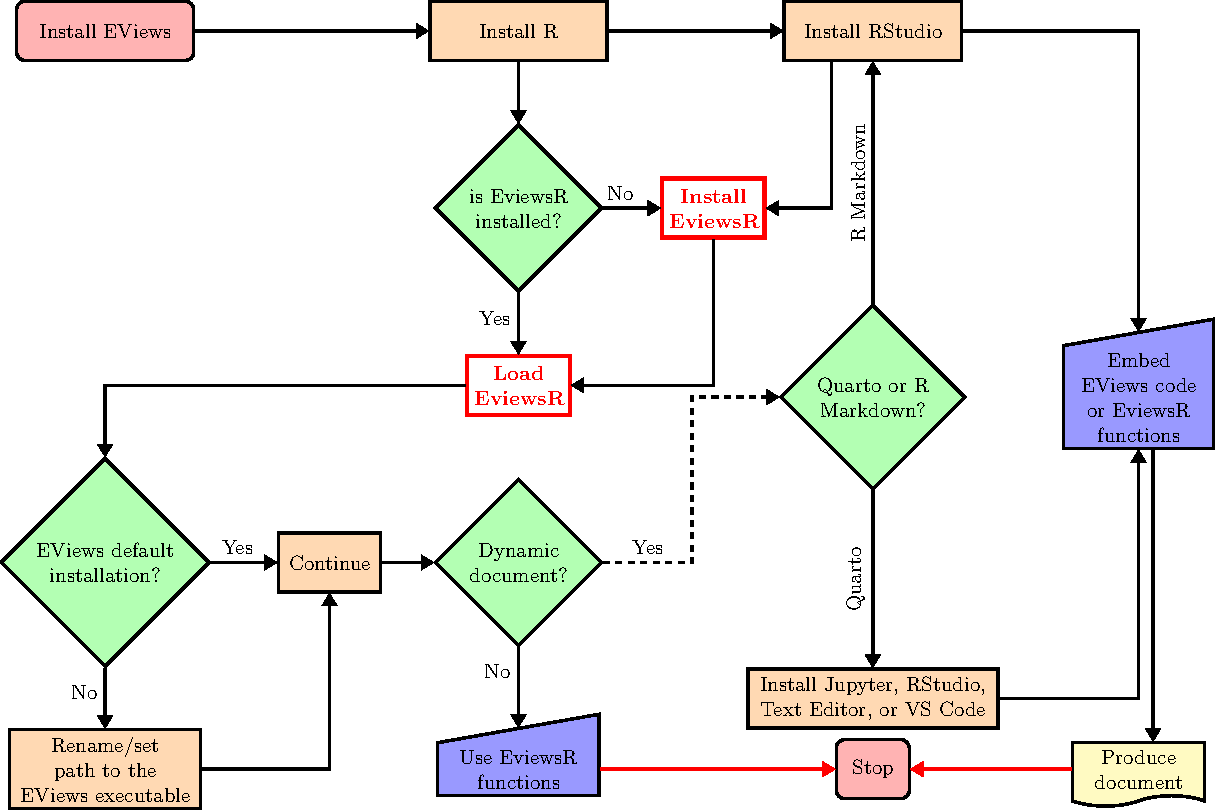
\includegraphics[height=0.3\textheight]{EviewsR_files/figure-latex/fig-flowchart-1} 

}

\caption{Setting up EviewsR, EViews, R, R Markdown and Quarto}\label{fig:fig-flowchart}
\end{figure}

\hypertarget{sec-document}{%
\section{EviewsR: R Markdown and Quarto document}\label{sec-document}}

As mentioned earlier, the \CRANpkg{EviewsR} package adds \texttt{eviews} as a knit-engine to \CRANpkg{knitr} package. Therefore, it allows users to embed EViews code in an R Markdown or Quarto document. After loading the package, then create an EViews chunk as shown below:

\begin{verbatim}
```{eviews}     
#| label: fig-EviewsR
#| graph: ""
#| eval: true
#| echo: false


  'This is some comment in EViews program, feel free to write anything
  
  wfcreate(wf=EviewsR,page=EviewsR) m 2000 2022

  for %y EviewsR1 EviewsR2
  pagecreate(page={%y}) m 2000 2022
  next

  for %y EviewsR EviewsR1 EviewsR2
  
  pageselect {%y}
  
  genr y=@cumsum(nrnd)
  genr x=@cumsum(nrnd)
  
  graph x_graph.line(o=eviews5) x
  graph y_graph.dot(o=bokeh) y
  
  table EviewsRTable

  for !j=1 to 7
  EviewsRTable(1,{!j})="Header"+" "+@str({!j})
  next

  for !i=1 to 10
  for !j=1 to 7
  EviewsRTable({!i}+1,{!j})=@str({!i})+","+@str({!j})
  next
  next 

  next
  
  wfsave EviewsR_files/EviewsR
```  
\end{verbatim}

The above EViews chunk creates an EViews program with the chunk's content, then automatically opens EViews and runs the program, which will create an EViews workfile with pages (\texttt{EviewsR}, \texttt{EviewsR1}, and \texttt{EviewsR2}) each containing random walk series x and y from January, 2000 to December, 2022. The program will also save an EViews workfile named \texttt{EviewsR.wf1} in the current directory. We believe that elaboration on the chunk header and options is in order. The word \texttt{eviews} tells the chunk to execute using EViews code, \texttt{fig-EviewsR} is the chunk's label, \texttt{"eval:\ true"} asks the chunk to evaluate the content (code) of the chunk, \texttt{"echo:\ true"} allows the content of the chunk to appear in the final document output, \texttt{comment:\ NULL} eliminates the comment prefix in the chunk output. We set \texttt{\textquotesingle{}graph:\ ""\textquotesingle{}} in order not show any EViews graph objects. Please refer to \CRANpkg{knitr}'s documentation for details. Table \ref{tab:tbl-chunkOptions} lists the specific chunk options for \CRANpkg{EviewsR} package:

\begin{table}[!h]

\caption{\label{tab:tbl-chunkOptions}The chunk options available for EviewsR package in R Markdown and Quarto documents}
\centering
\resizebox{\linewidth}{!}{
\begin{tabular}[t]{>{}ll>{\raggedright\arraybackslash}p{4cm}>{\raggedright\arraybackslash}p{4cm}>{\raggedright\arraybackslash}p{4cm}}
\toprule
\textbf{Chunk option} & \textbf{Default value} & \textbf{Possible values} & \textbf{Example} & \textbf{Meaning}\\
\midrule
\textbf{equation} & * & Any valid name pattern for EViews @wlookup function & eq*, ??e, *e* & EViews equation object\\
\textbf{graph} & * & asis, first, last, asc, desc, or any valid name pattern for EViews @wlookup function & gr*, g??, *t* & EViews graph object\\
\textbf{series} & * & Any valid name pattern for EViews `@wlookup` function & se*, ?e?, *y* & EViews series object\\
\textbf{table} & * & Any valid name pattern for EViews @wlookup function & ta*, ?t, *s* & EViews table object\\
\textbf{page} & * & Any valid name pattern for EViews @wlookup function & page1, page2, page3, page4, page5 & EViews page\\
\textbf{graph\_procs} &  & Any valid EViews graph's procedure & align(2,1,1) & EViews graph's procedure\\
\textbf{save\_options} &  & Any valid options for EViews save command & t=pdf, -c & EViews options for graph save command\\
\textbf{class} & df & xts &  & Class of R's object for imported EViews series objects\\
\textbf{save\_path} &  & Any valid path & C:/Users/EviewsR & Path to save EViews graphs\\
\bottomrule
\end{tabular}}
\end{table}

\hypertarget{sec-dynamic}{%
\section{EviewsR: Dynamic Document}\label{sec-dynamic}}

This section is about working with EViews's equation, graph, series and table objects dynamically in an R Markdown or Quarto document.

\hypertarget{accessing-eviews-objects-from-eviews-chunk}{%
\subsection{Accessing EViews objects from EViews chunk}\label{accessing-eviews-objects-from-eviews-chunk}}

The EViews chunk below (\texttt{label:\ fig-EviewsR1}) contains EViews code which generates a workfile named \texttt{EviewsR\_workfile} along with a page \texttt{EviewsR\_page} with monthly frequency from 2000 2022. The chunk also creates additional three EViews pages (\texttt{page1}, \texttt{page2}, and \texttt{EviewsR}) and generates three series objects \(x\), \(y\) and \(z\). It then runs the ordinary least square (OLS) method with \(y\) as the dependent variable and the rest as independent variables on each of the new pages. On each of the new pages, an equation, a table and three graph objects are created. The equation object is defined as \texttt{OLS}, the table object as \texttt{OLS\_TABLE} and three graph objects as \texttt{graph1}, \texttt{graph2} and \texttt{graph3}.

The chunk automatically creates a new environment with the chunk's label as the environment's name, then returns all the EViews's equation, series and table objects into R as a dataframe saved within the new environment. Note that the chunk label (\texttt{fig-EviewsR1}) is not a valid R object, so \CRANpkg{EviewsR} removes the prefix \texttt{fig-} before creating the new environment as \texttt{EviewsR1}. The prefix (\texttt{fig-}) is added to the chunk label because it is the Quarto's default way to wrap plots contained in a chunk in a figure environment for cross-reference. If you are working with R Markdown or the chunk does not contain EViews graph objects, you do not need to add the prefix.

The contents of the EViews \texttt{table} objects are imported into R exactly as they are on the EViews workfile, but the table name is changed to small letters. You can use the following format to get the imported table:

\begin{itemize}
\tightlist
\item
  \texttt{chunkLabel\$pageName\_tableName}
\end{itemize}

The \texttt{chunkLabel} stands for the chunk label and is the new environment, \texttt{pageName} for the EViews page name and \texttt{tableName} for the EViews table object. Therefore, \texttt{EviewsR1\$eviewsr\_ols\_table} accesses the table \texttt{ols\_table}, which is imported from \texttt{EviewsR} page of chunk \texttt{EviewsR1} into R as a dataframe.

\begin{verbatim}
```{eviews} 
#| label: fig-EviewsR1
#| fig.cap: EViews graphs automatically imported by EViews chunk (fig-EviewsR1: default chunk options)
#| out.width: 32%
#| out.height: 15%
#| fig.ncol: 3
#| echo: false
#| eval: true

'This is some comment in EViews program, feel free to write anything

wfcreate(page=EviewsR_page,wf=EviewsR_workfile) m 2000 2022

!n=123

for %y page2 EviewsR  page1 
pagecreate(page={%y}) q 2000 2022
pageselect {%y}
rndseed !n
!n=!n+100

genr x=@cumsum(nrnd)
genr y=@cumsum(nrnd)
genr z=@cumsum(nrnd)
equation OLS.ls y c x z
freeze(OLS_TABLE,mode=overwrite) OLS
delete(noerr) GRAPH*
freeze(GRAPH3,mode=overwrite) z.line
graph GRAPH2.dot y
graph GRAPH1.area x
graph3.addtext(ar) %y
graph2.addtext(ar) %y
graph1.addtext(ar) %y
next
``` 
\end{verbatim}

\begin{figure}

{\centering 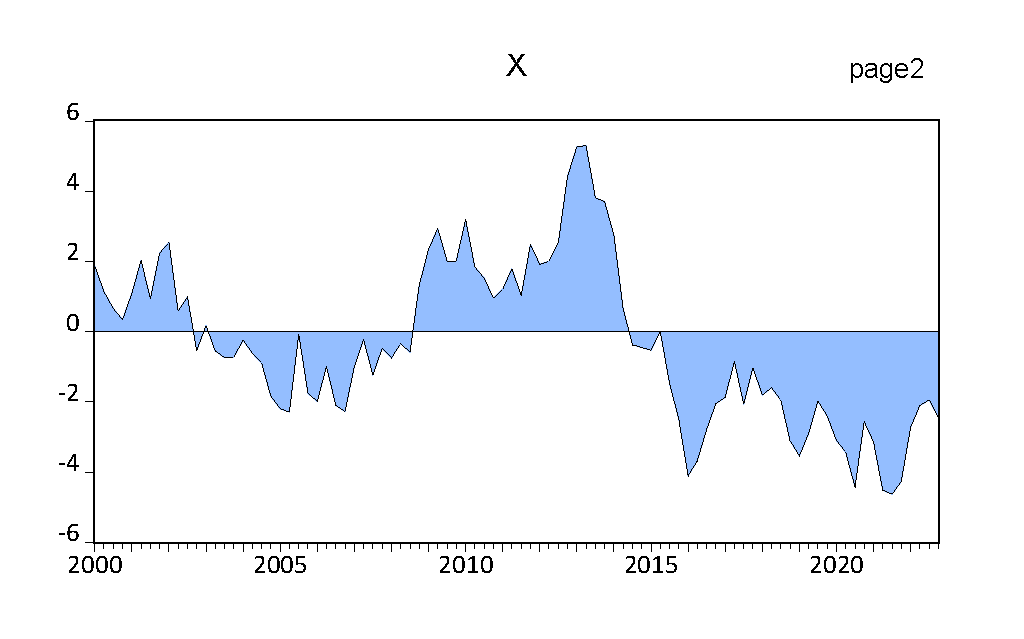
\includegraphics[width=0.32\linewidth,height=0.15\textheight]{figures/eviewsr1page2-graph1} 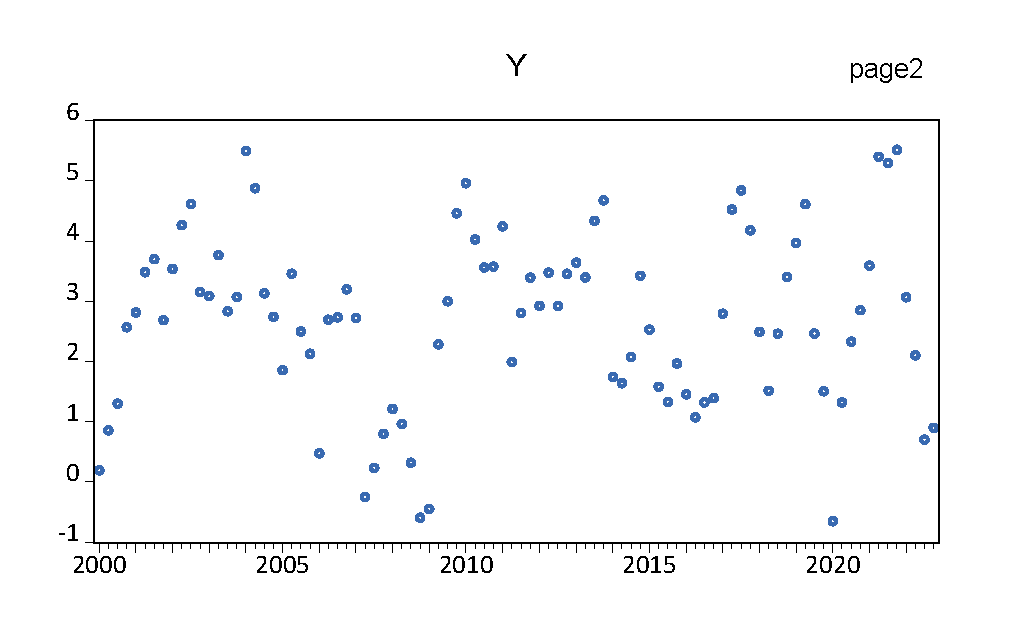
\includegraphics[width=0.32\linewidth,height=0.15\textheight]{figures/eviewsr1page2-graph2} 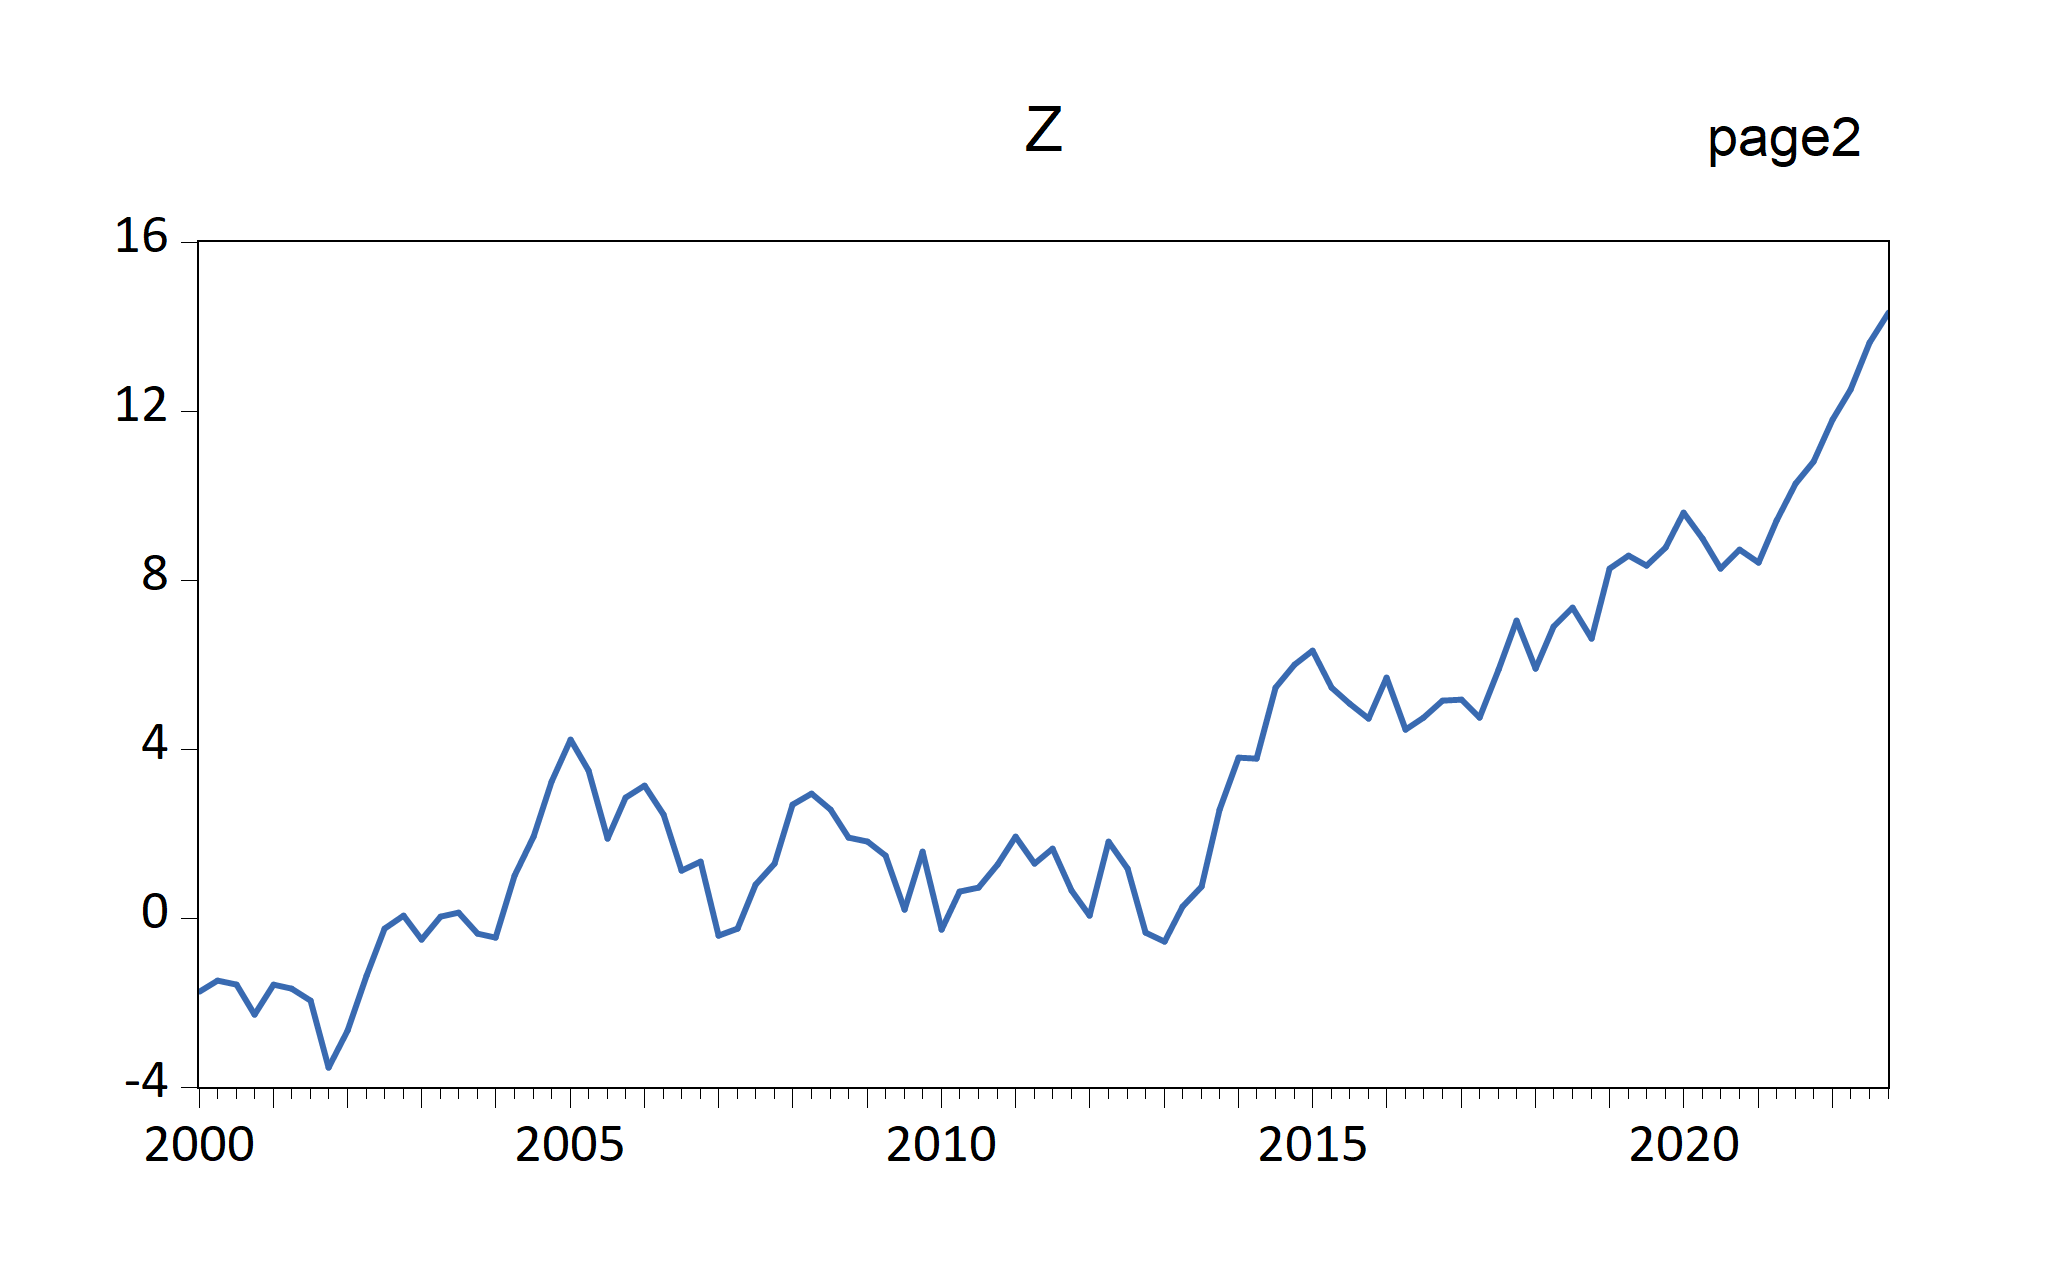
\includegraphics[width=0.32\linewidth,height=0.15\textheight]{figures/eviewsr1page2-graph3} 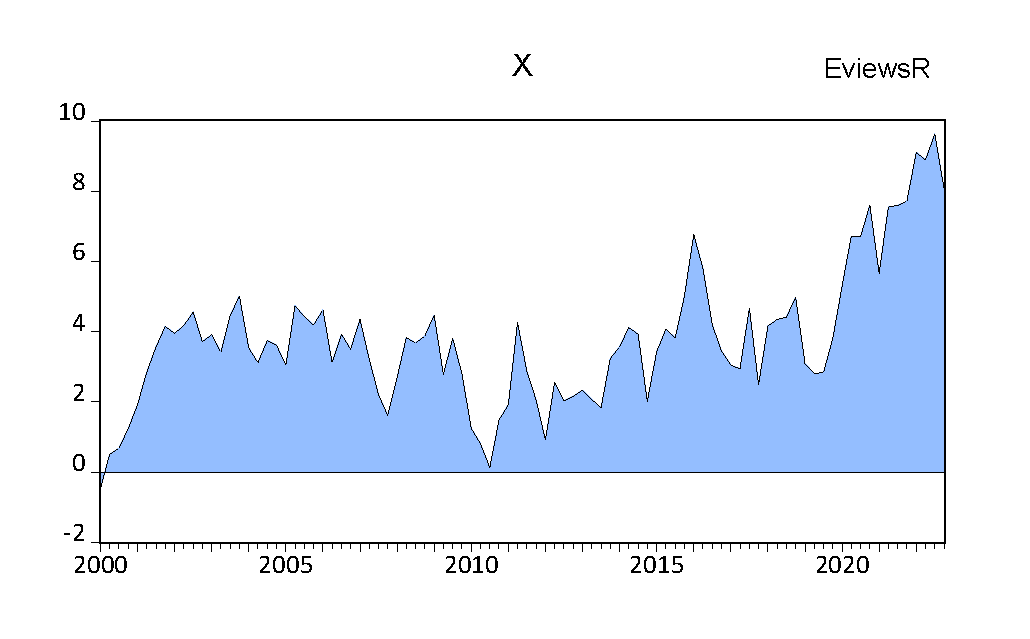
\includegraphics[width=0.32\linewidth,height=0.15\textheight]{figures/eviewsr1eviewsr-graph1} 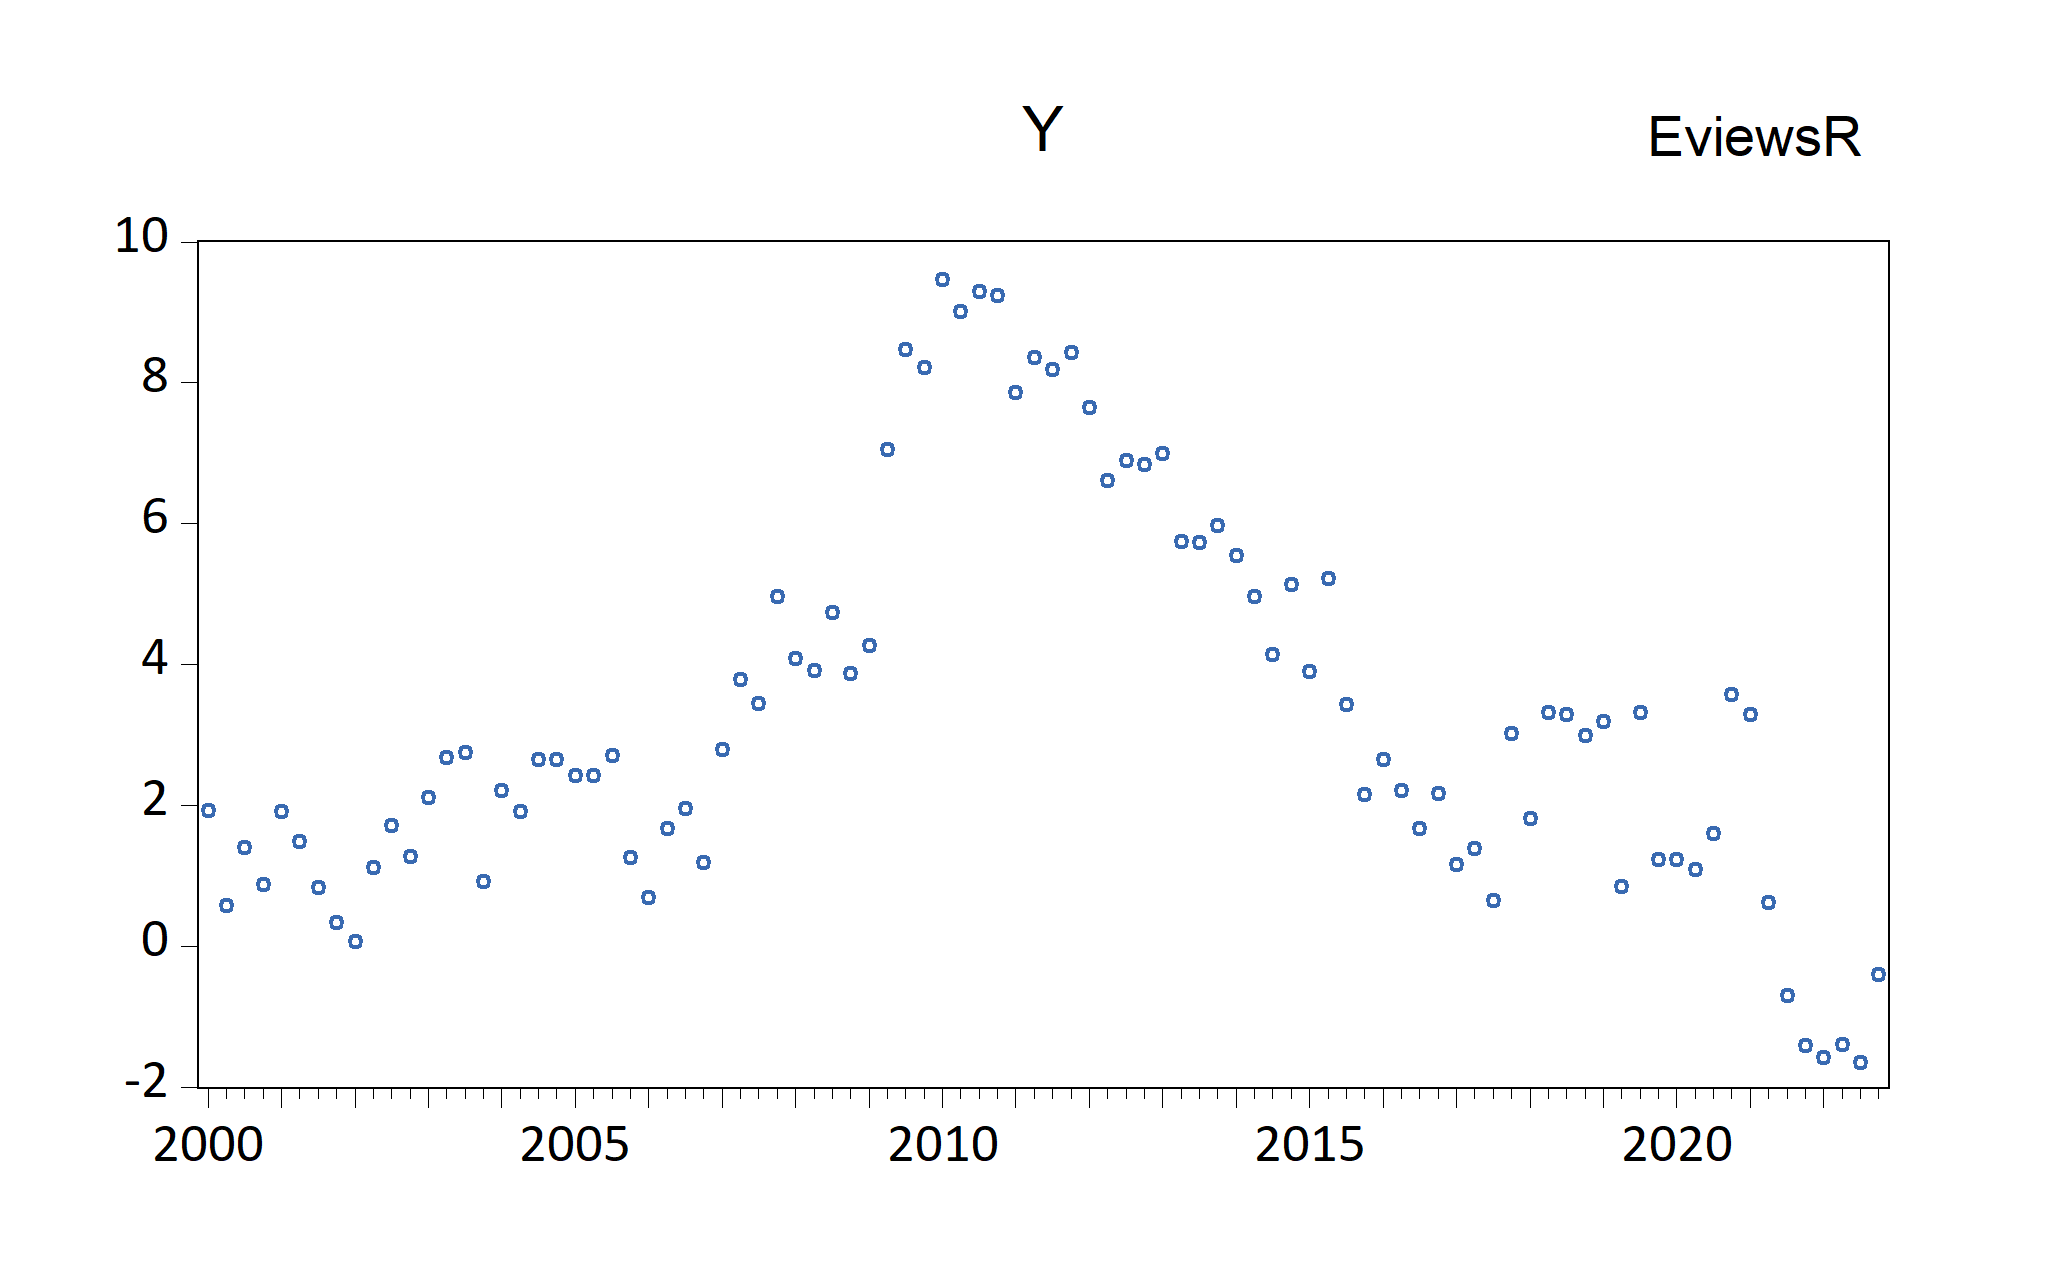
\includegraphics[width=0.32\linewidth,height=0.15\textheight]{figures/eviewsr1eviewsr-graph2} 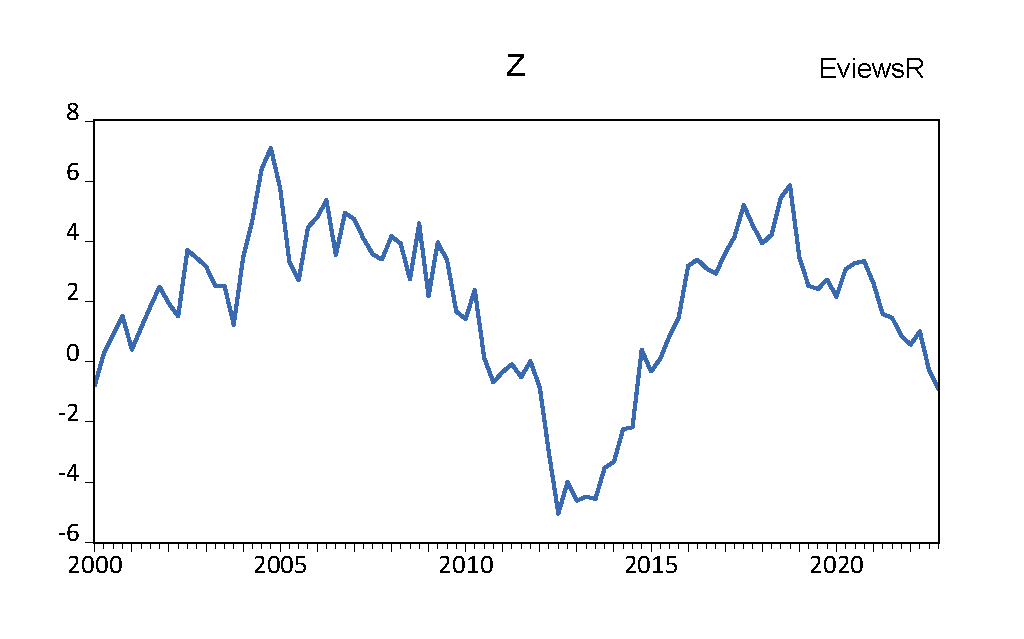
\includegraphics[width=0.32\linewidth,height=0.15\textheight]{figures/eviewsr1eviewsr-graph3} 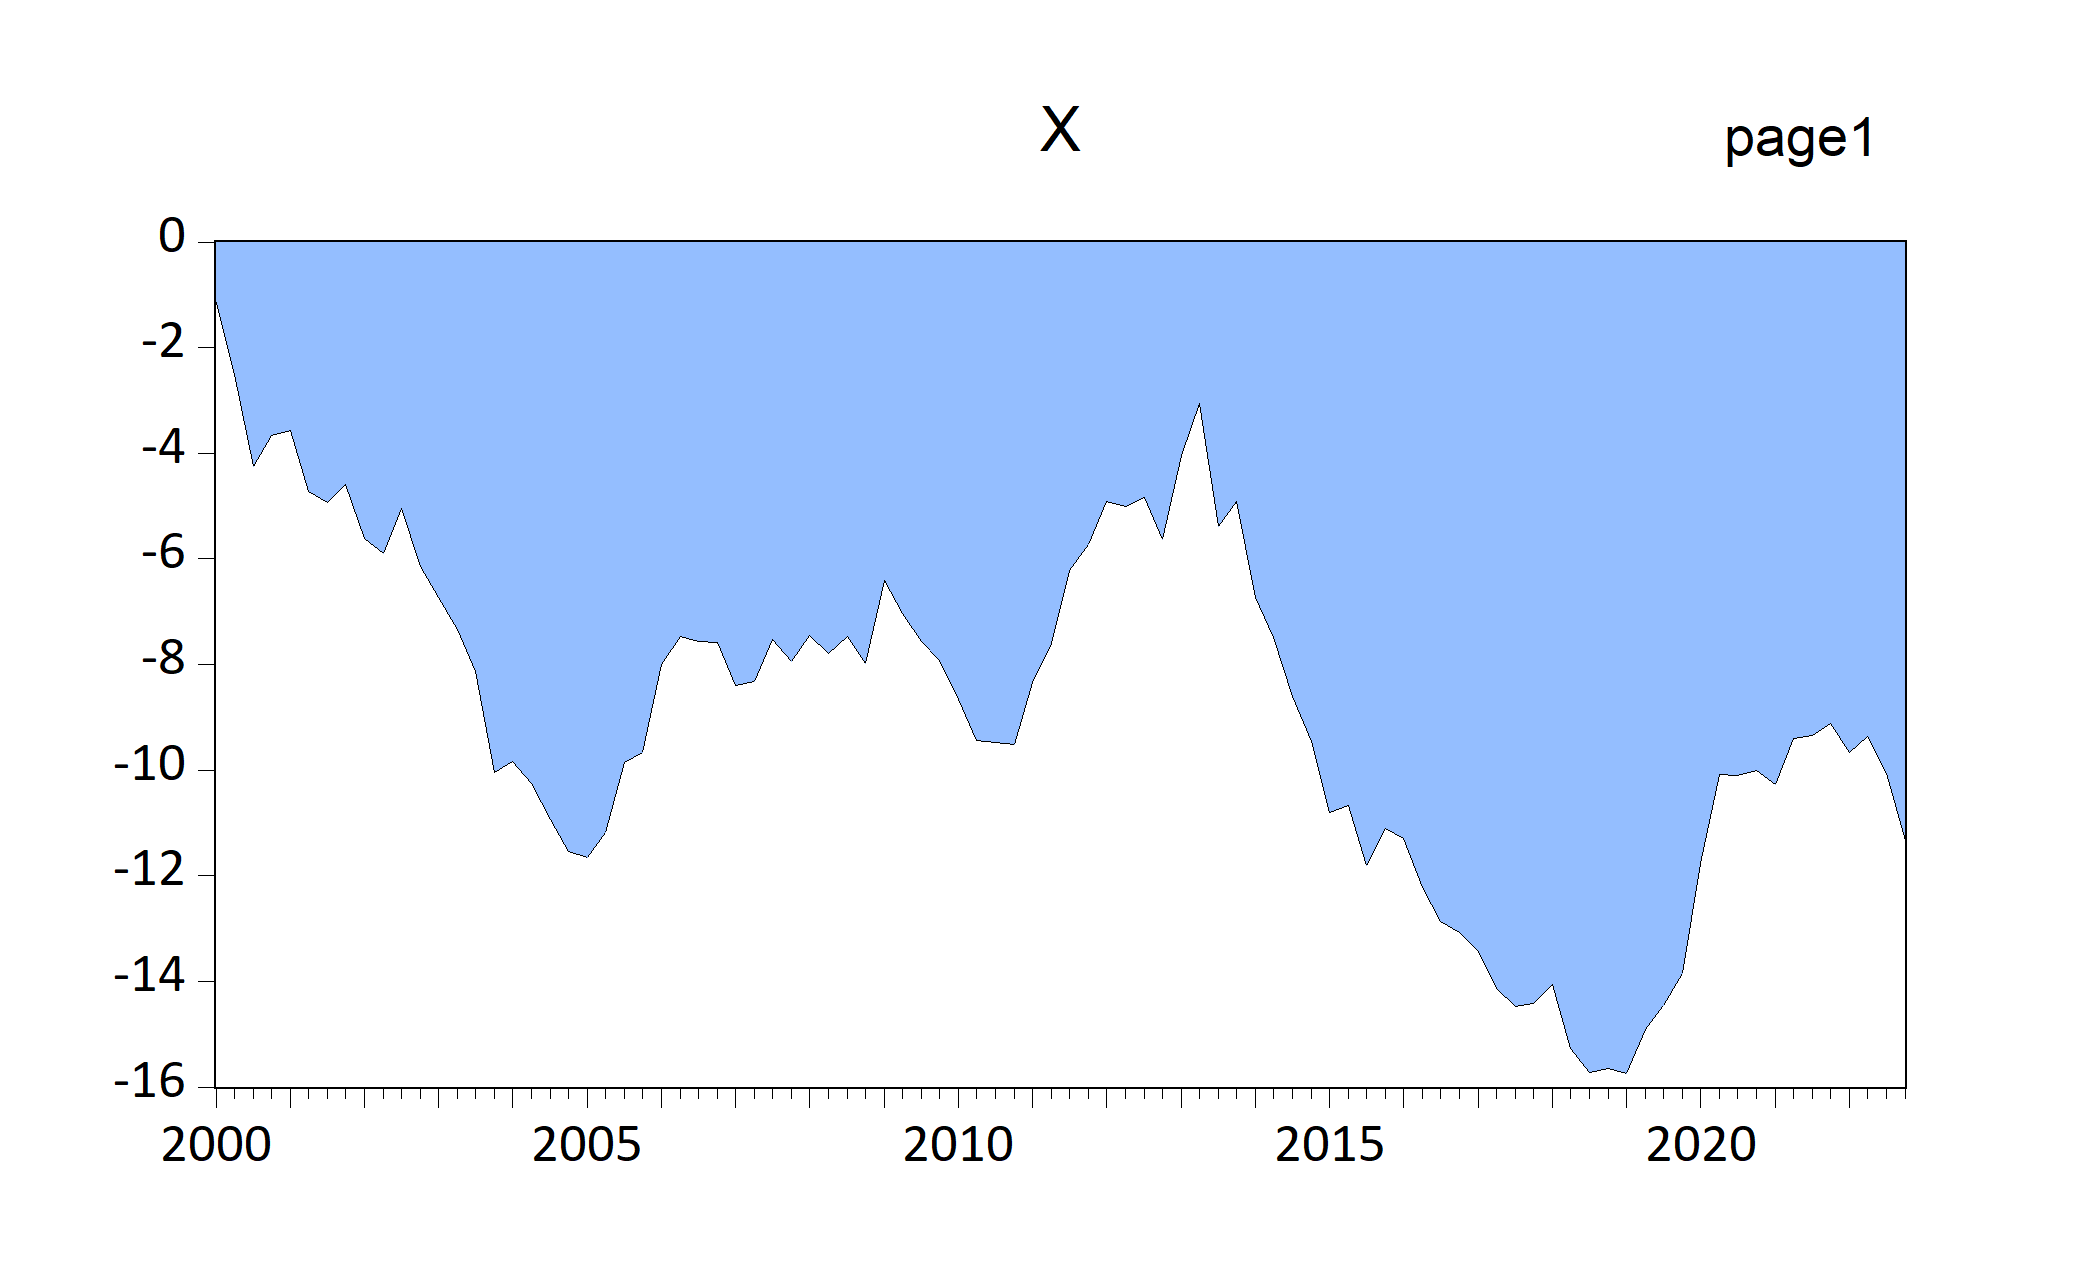
\includegraphics[width=0.32\linewidth,height=0.15\textheight]{figures/eviewsr1page1-graph1} 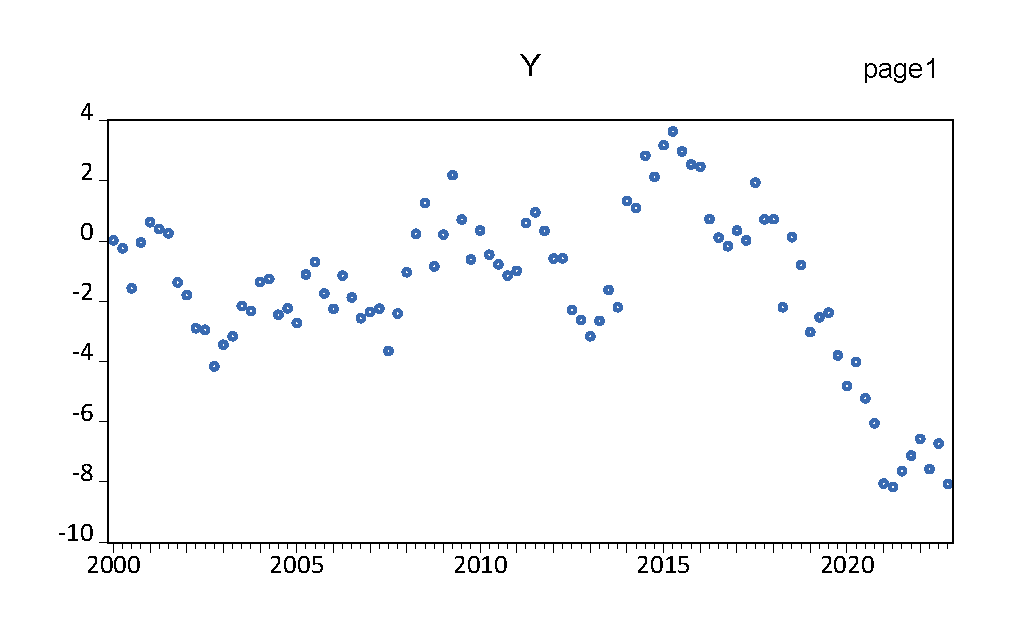
\includegraphics[width=0.32\linewidth,height=0.15\textheight]{figures/eviewsr1page1-graph2} 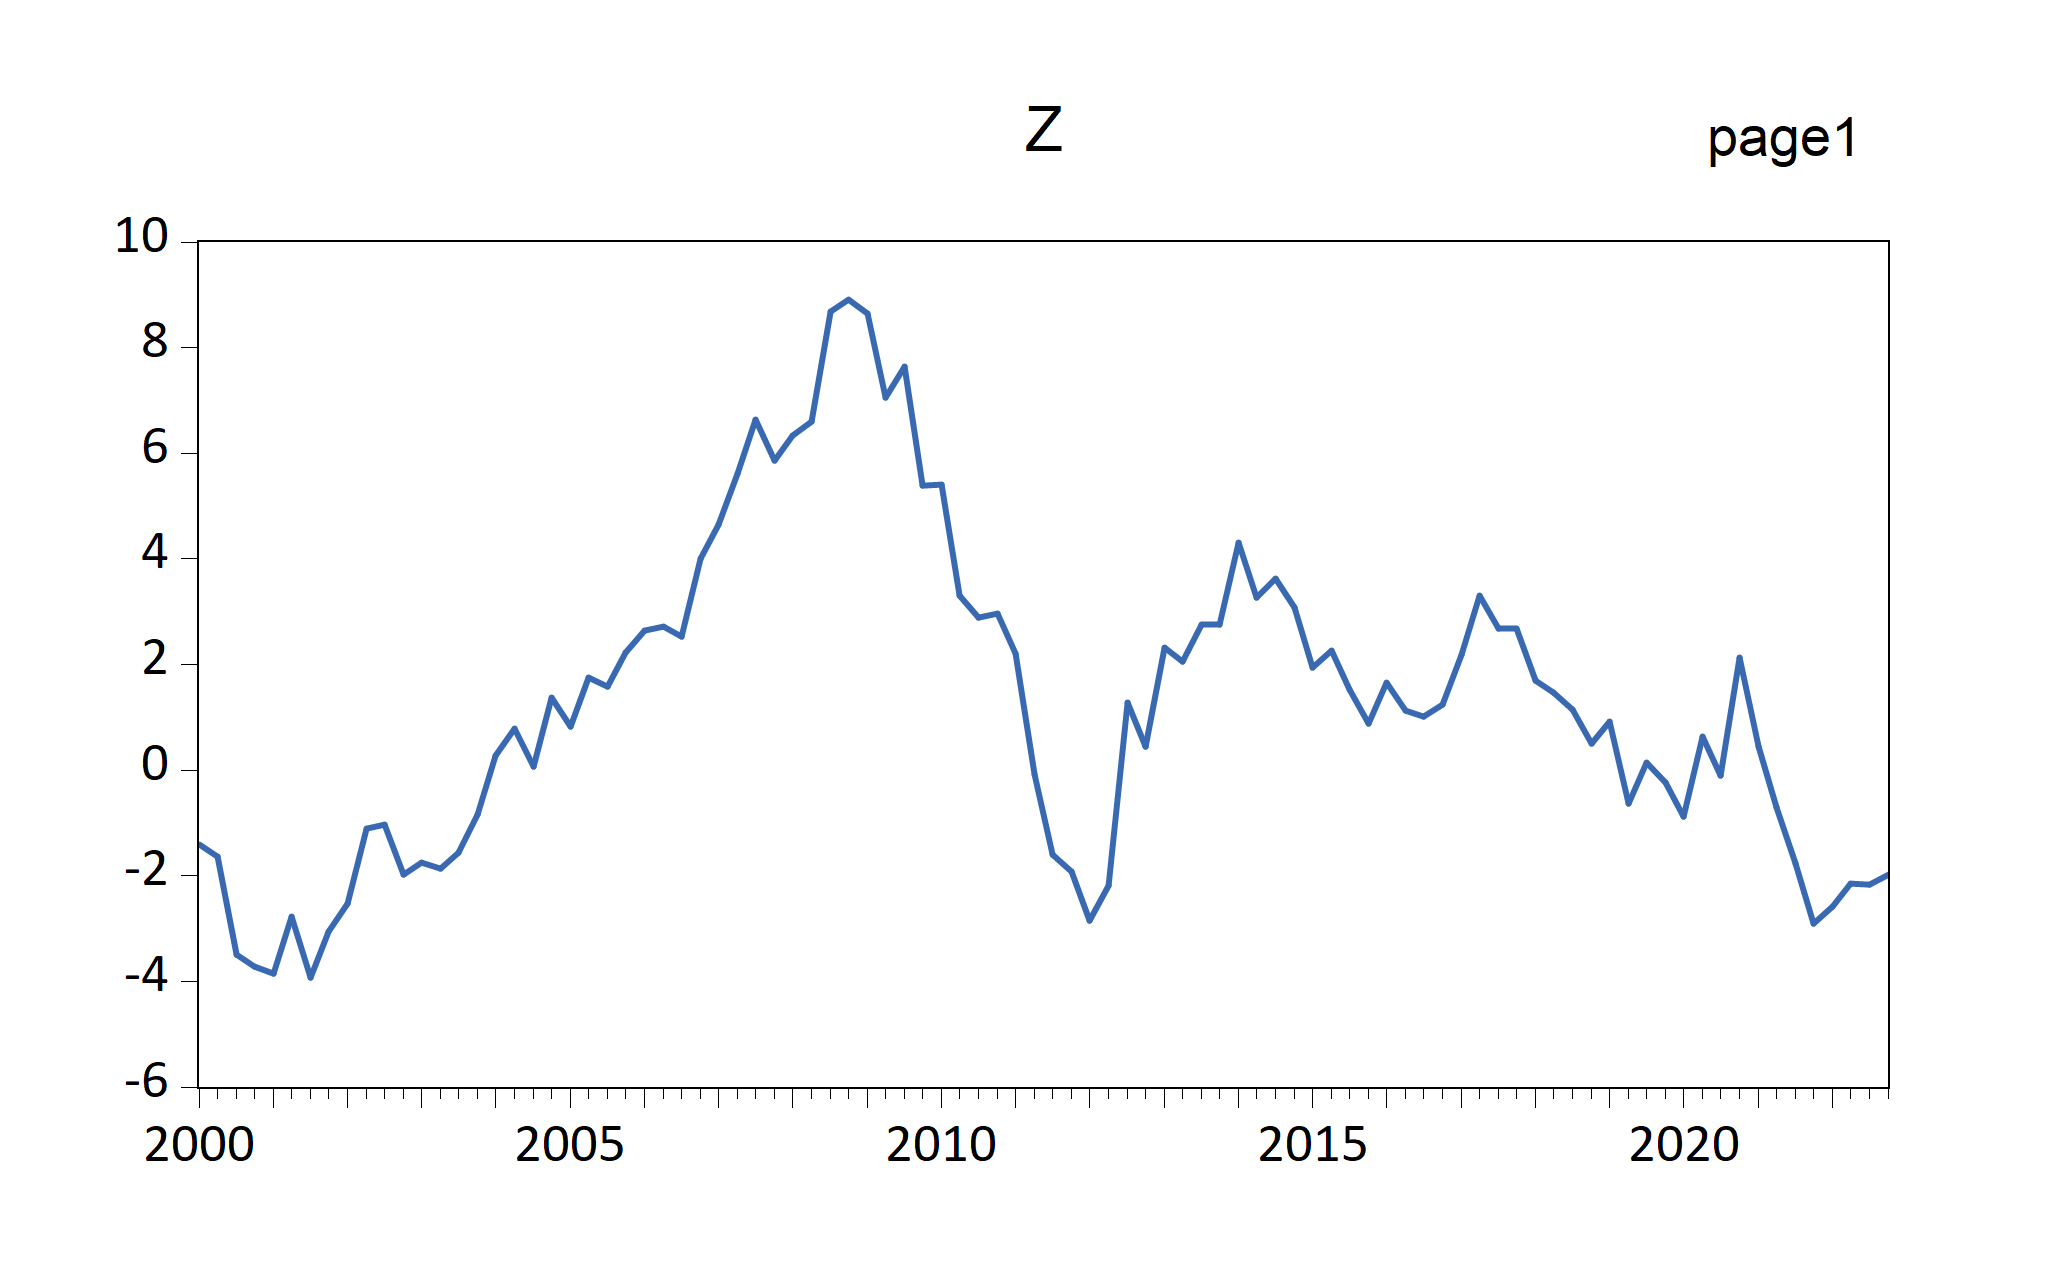
\includegraphics[width=0.32\linewidth,height=0.15\textheight]{figures/eviewsr1page1-graph3} 

}

\caption{EViews graphs automatically imported by EViews chunk (fig-EviewsR1: default chunk options)}\label{fig:fig-EviewsR1-1}
\end{figure}

On the other hand, some data members of the EViews \texttt{equation} objects are extracted and imported into the new environment as a dataframe. Data member' is an EViews term for statistics, summaries, and information criteria related to EViews \texttt{equation} objects. The code below shows the general way to access the imported equation object, where \texttt{equationName} is the EViews equation object. The page and equation names are separated by underscore (\texttt{\_}).
The data members of the equation objects can be accessed via standard list element access syntax:

\begin{itemize}
\tightlist
\item
  \texttt{chunkLabel\$pageName\_equationName\$dataMember}
\end{itemize}

For example, the \(R^2\) value of the OLS equation object on \texttt{EviewsR} page is 0.402377, which can be accessed using the inline expression \texttt{\textasciigrave{}r\ EviewsR1\$eviewsr\_ols\$r2\textasciigrave{}}.

Note that \texttt{@coefs}, \texttt{@pval}, \texttt{@stderrs} and \texttt{@tstats} return vectors with length equal to the number of estimated coefficients. The second value of each of these vectors can be accessed with typical square bracket notation, i.e.~by appending \texttt{{[}2{]}}. The rest of the data members return scalar values. The number of data members reported by the EviewsR package is greater than that provided by \texttt{lm()}, \texttt{glm()} and \texttt{summary()} R functions. For example, R users need to use more functions or lines of code to get the values of Schwarz and Hannan-Quinn Information Criteria of an estimated model. These values are automatically imported into R, R Markdown or Quarto environment by the EviewsR package.

The graph objects are saved on disk to the path defined by the chunk option \texttt{fig.path} and can be captioned and sub-captioned via the chunk options \texttt{fig.cap} (\texttt{fig-cap}) and \texttt{fig.subcap} (\texttt{fig-subcap}) in an R Markdown (Quarto) document. The graph file on the disk are named in the following format:

\begin{itemize}
\tightlist
\item
  \texttt{chunkLabel-pageName-graphName}
\end{itemize}

For example, \texttt{eviewsr1-page2-graph1} is the name of \texttt{graph1} object of \texttt{page2} created in \texttt{fig-EviewsR1} chunk.

The series objects of each page can be fetched through

\begin{itemize}
\tightlist
\item
  \texttt{chunkLabel\$pageName}.
\end{itemize}

For example, \texttt{EviewsR1\$page2} provides the dataframe of all the series objects on \texttt{page2}. Even if the page is not defined in the created or imported workfile, EViews names both the workfile and page as \texttt{untitled} by default. So \texttt{EviewsR1\$untitled} is the right way to access the series object, if no page name is defined in the \texttt{fig-EviewsR1} chunk.

By default, \CRANpkg{EviewsR} imports the series objects as a dataframe with date column formatted as \texttt{POSIXct} . We can import the series objects as \texttt{xts} object by setting chunk option \texttt{class="xts"}.

Note that the chunk label is case-sensitive, while the EViews equation, series and table objects are not. They can be in capital letters in the chunk, but they are in lowercase in the R object. This is because R variable names are case-sensitive, while EViews objects are not. For consistency, \CRANpkg{EviewsR} is designed to convert EViews object names to lowercase. Therefore, we recommend naming EViews objects with lowercase names.

The graph objects in Figure \ref{fig:fig-EviewsR1-1} are imported with the default chunk options. We can use chunk options \texttt{page}, \texttt{graph} and \texttt{graph\_procs} to change the behaviour of the graphical outputs. The chunk option \texttt{page} can take \texttt{page="*"}, or a space-delimited (or a vector of) string wtih the names of EViews pages. Note that we ask EViews to write the page name on the top right corner of each graph. The chunk option \texttt{graph} can have the values such as \texttt{*}, \texttt{first}, \texttt{last}, \texttt{asis}, \texttt{asc}, \texttt{desc} or a numeric vector.

\hypertarget{importing-eviews-graph-asis}{%
\subsection{Importing EViews graph asis}\label{importing-eviews-graph-asis}}

\color{black}

We set these chunk options to get Figure \ref{fig:fig-EviewsR2-1}.

\begin{itemize}
\item
  \texttt{graph:\ "@asis"}
\item
  \texttt{graph\_procs:\ template\ newspaper}
\end{itemize}

The option \texttt{graph:\ "@asis"} makes sure that the graph objects are imported in the order they appear in the EViews chunk, that is \texttt{graph3} followed by \texttt{graph2} and \texttt{graph1}. This option is only useful in an R Markdown or Quarto document:

\begin{figure}

{\centering 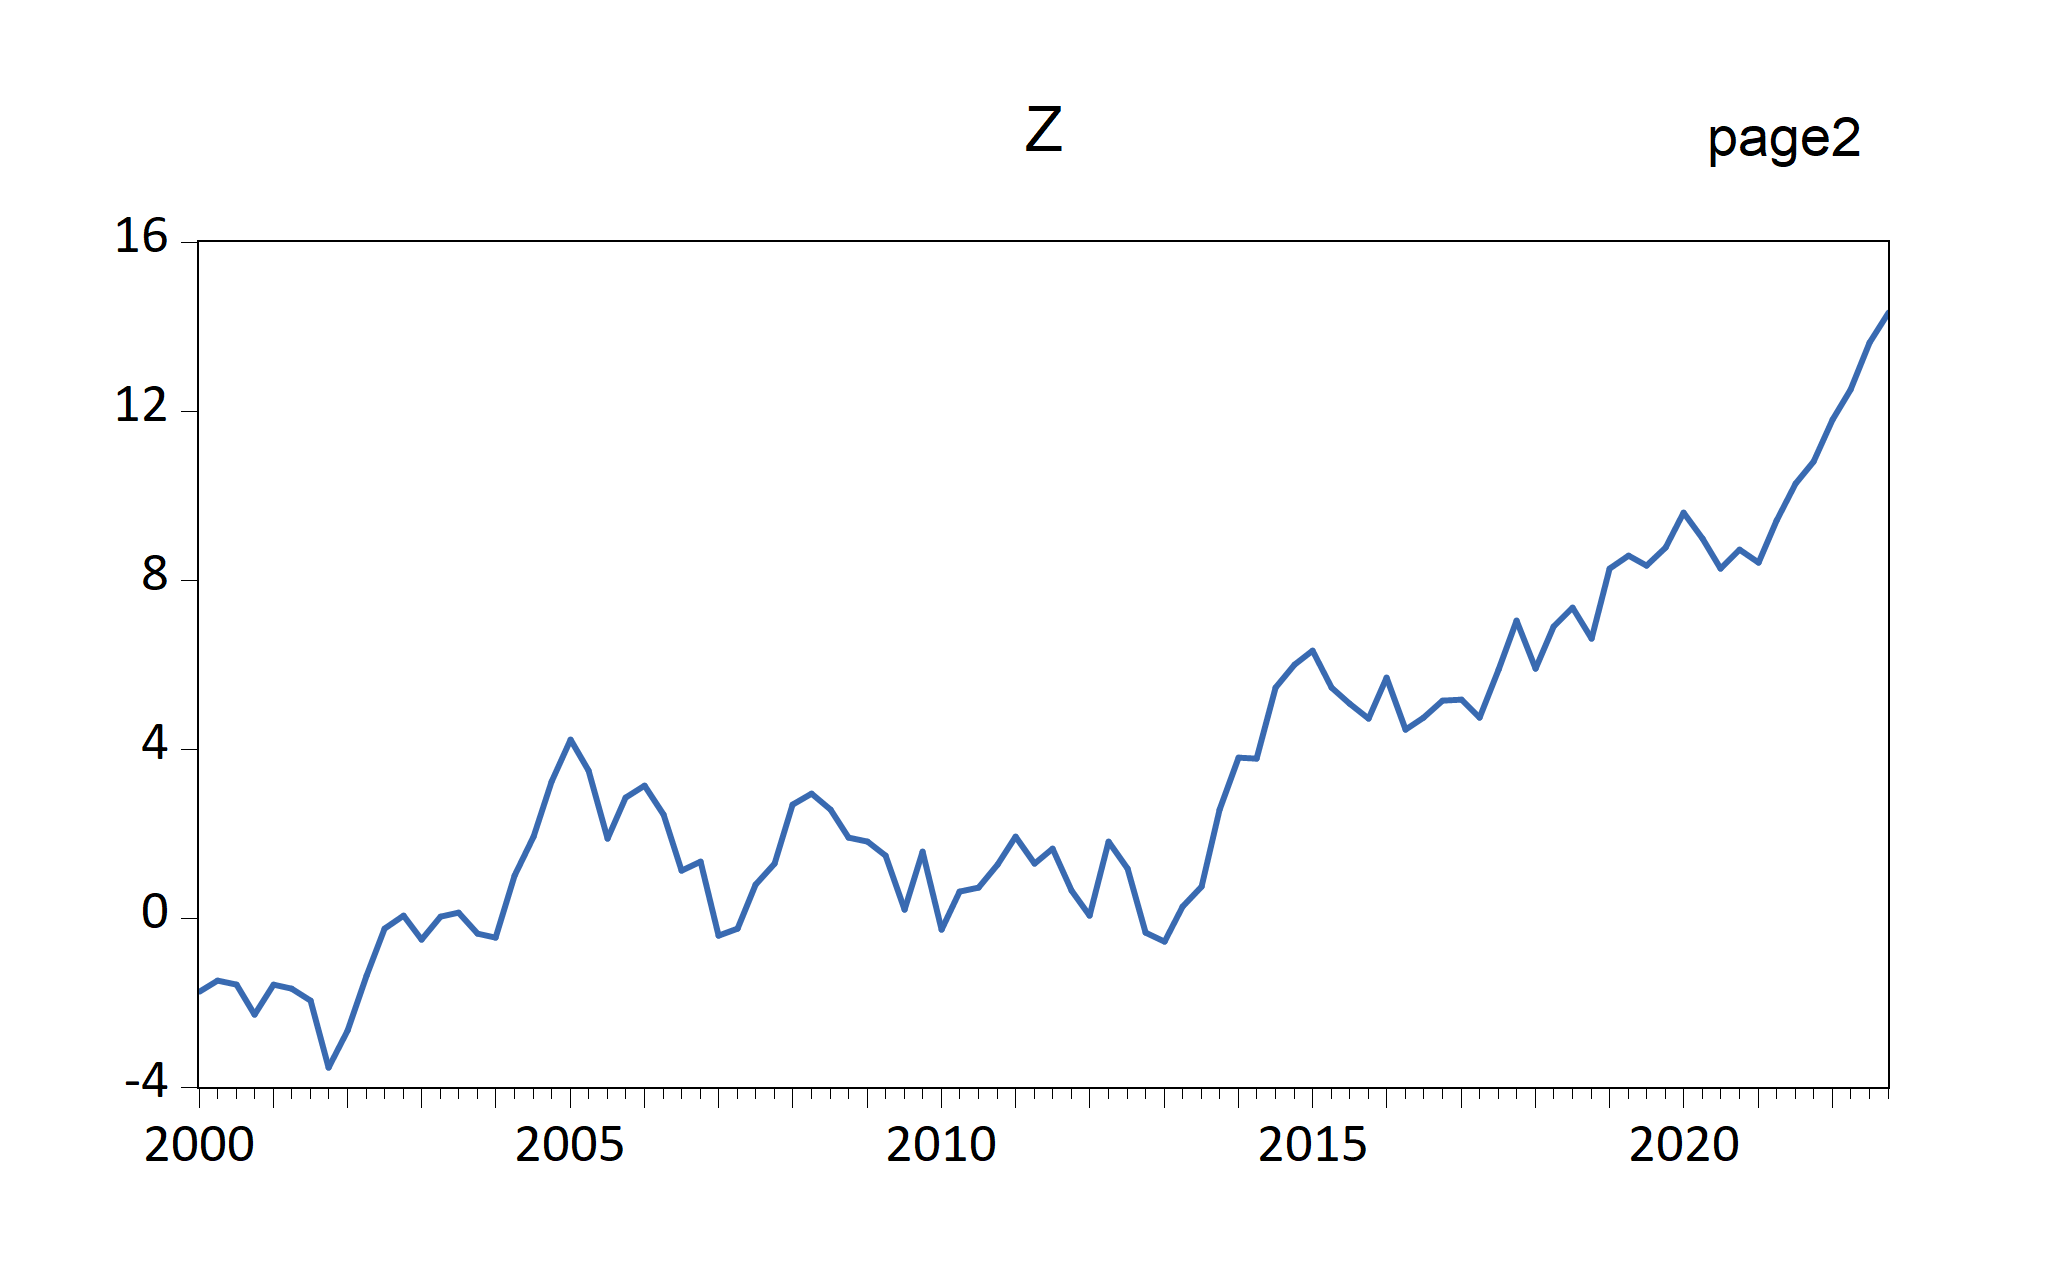
\includegraphics[width=0.32\linewidth,height=0.15\textheight]{figures/eviewsr1page2-graph3} 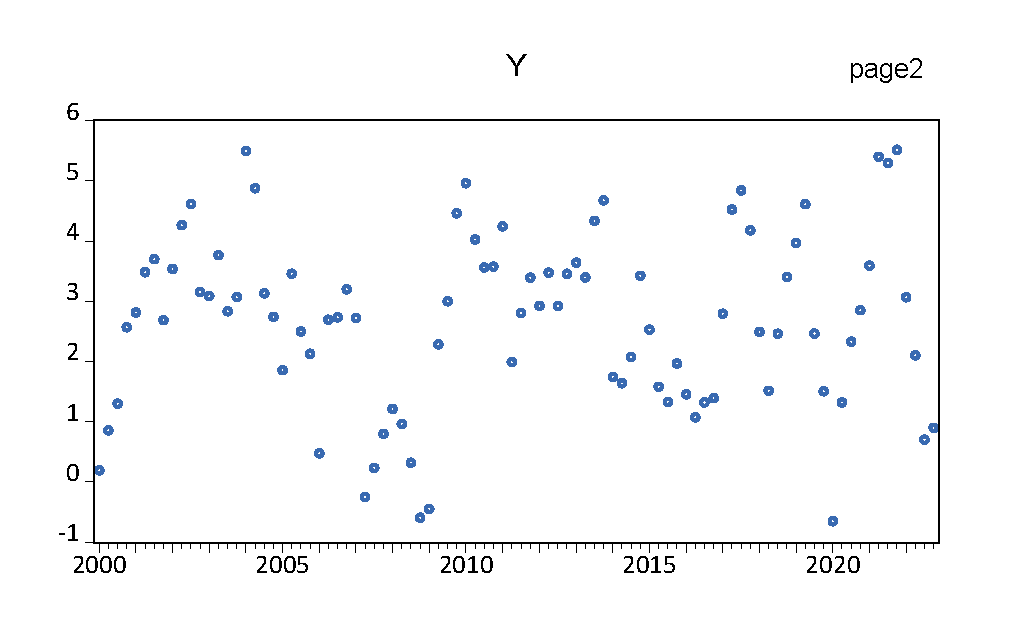
\includegraphics[width=0.32\linewidth,height=0.15\textheight]{figures/eviewsr1page2-graph2} 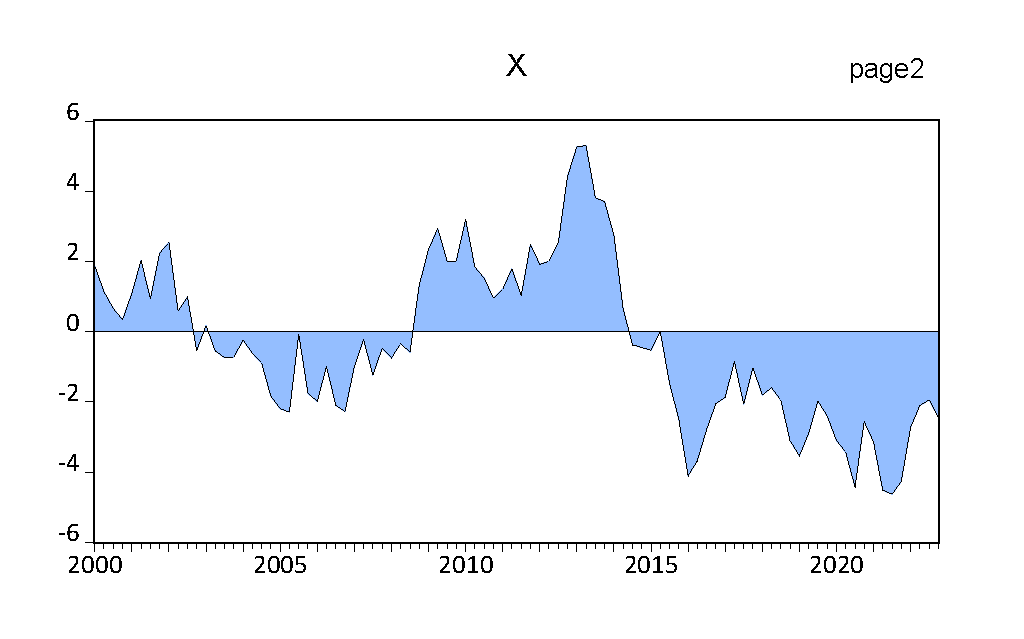
\includegraphics[width=0.32\linewidth,height=0.15\textheight]{figures/eviewsr1page2-graph1} 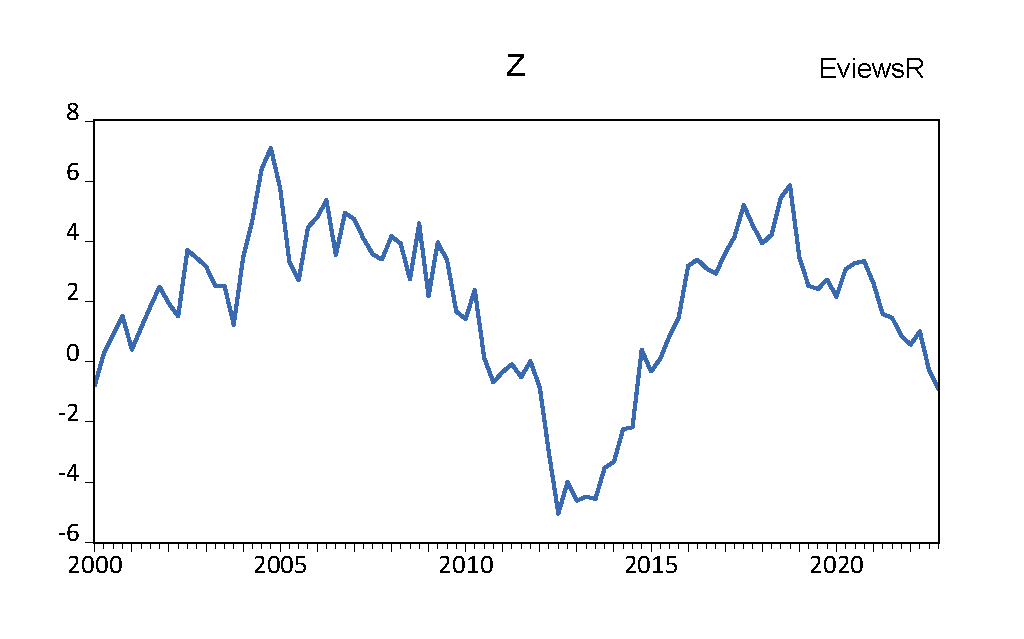
\includegraphics[width=0.32\linewidth,height=0.15\textheight]{figures/eviewsr1eviewsr-graph3} 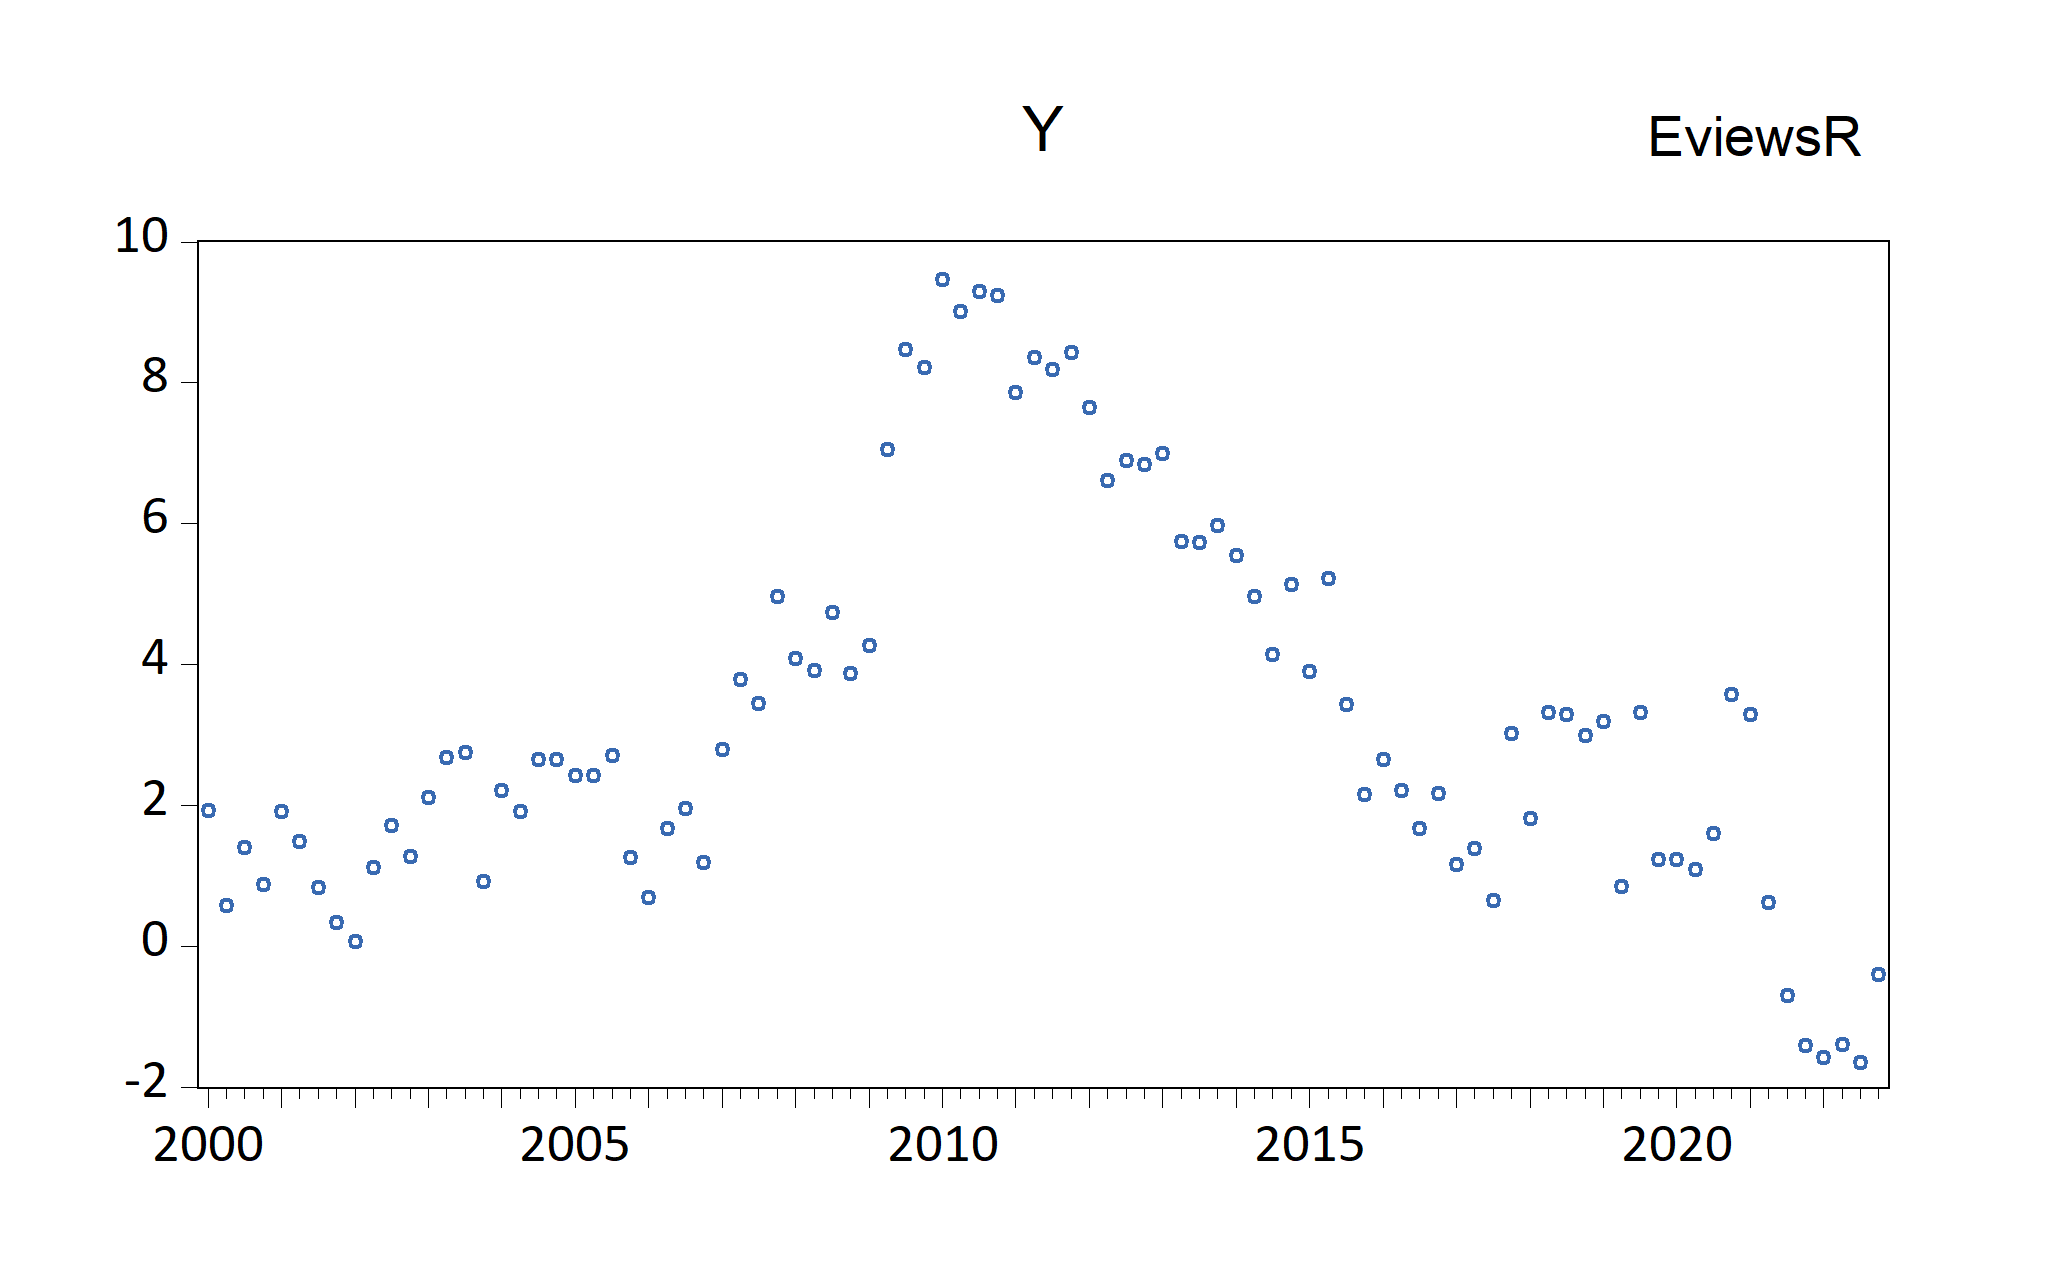
\includegraphics[width=0.32\linewidth,height=0.15\textheight]{figures/eviewsr1eviewsr-graph2} 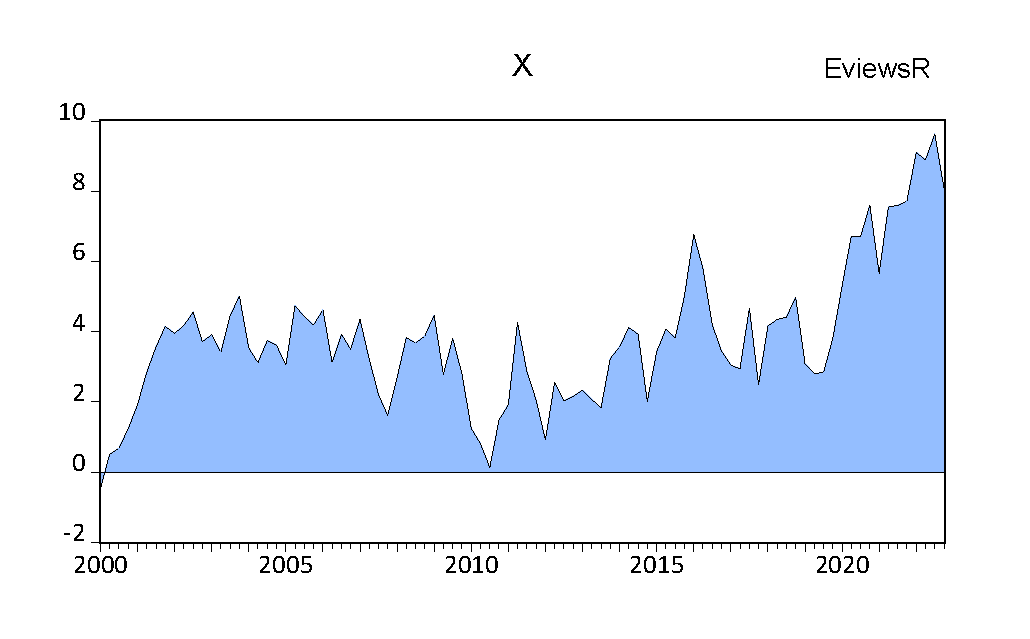
\includegraphics[width=0.32\linewidth,height=0.15\textheight]{figures/eviewsr1eviewsr-graph1} 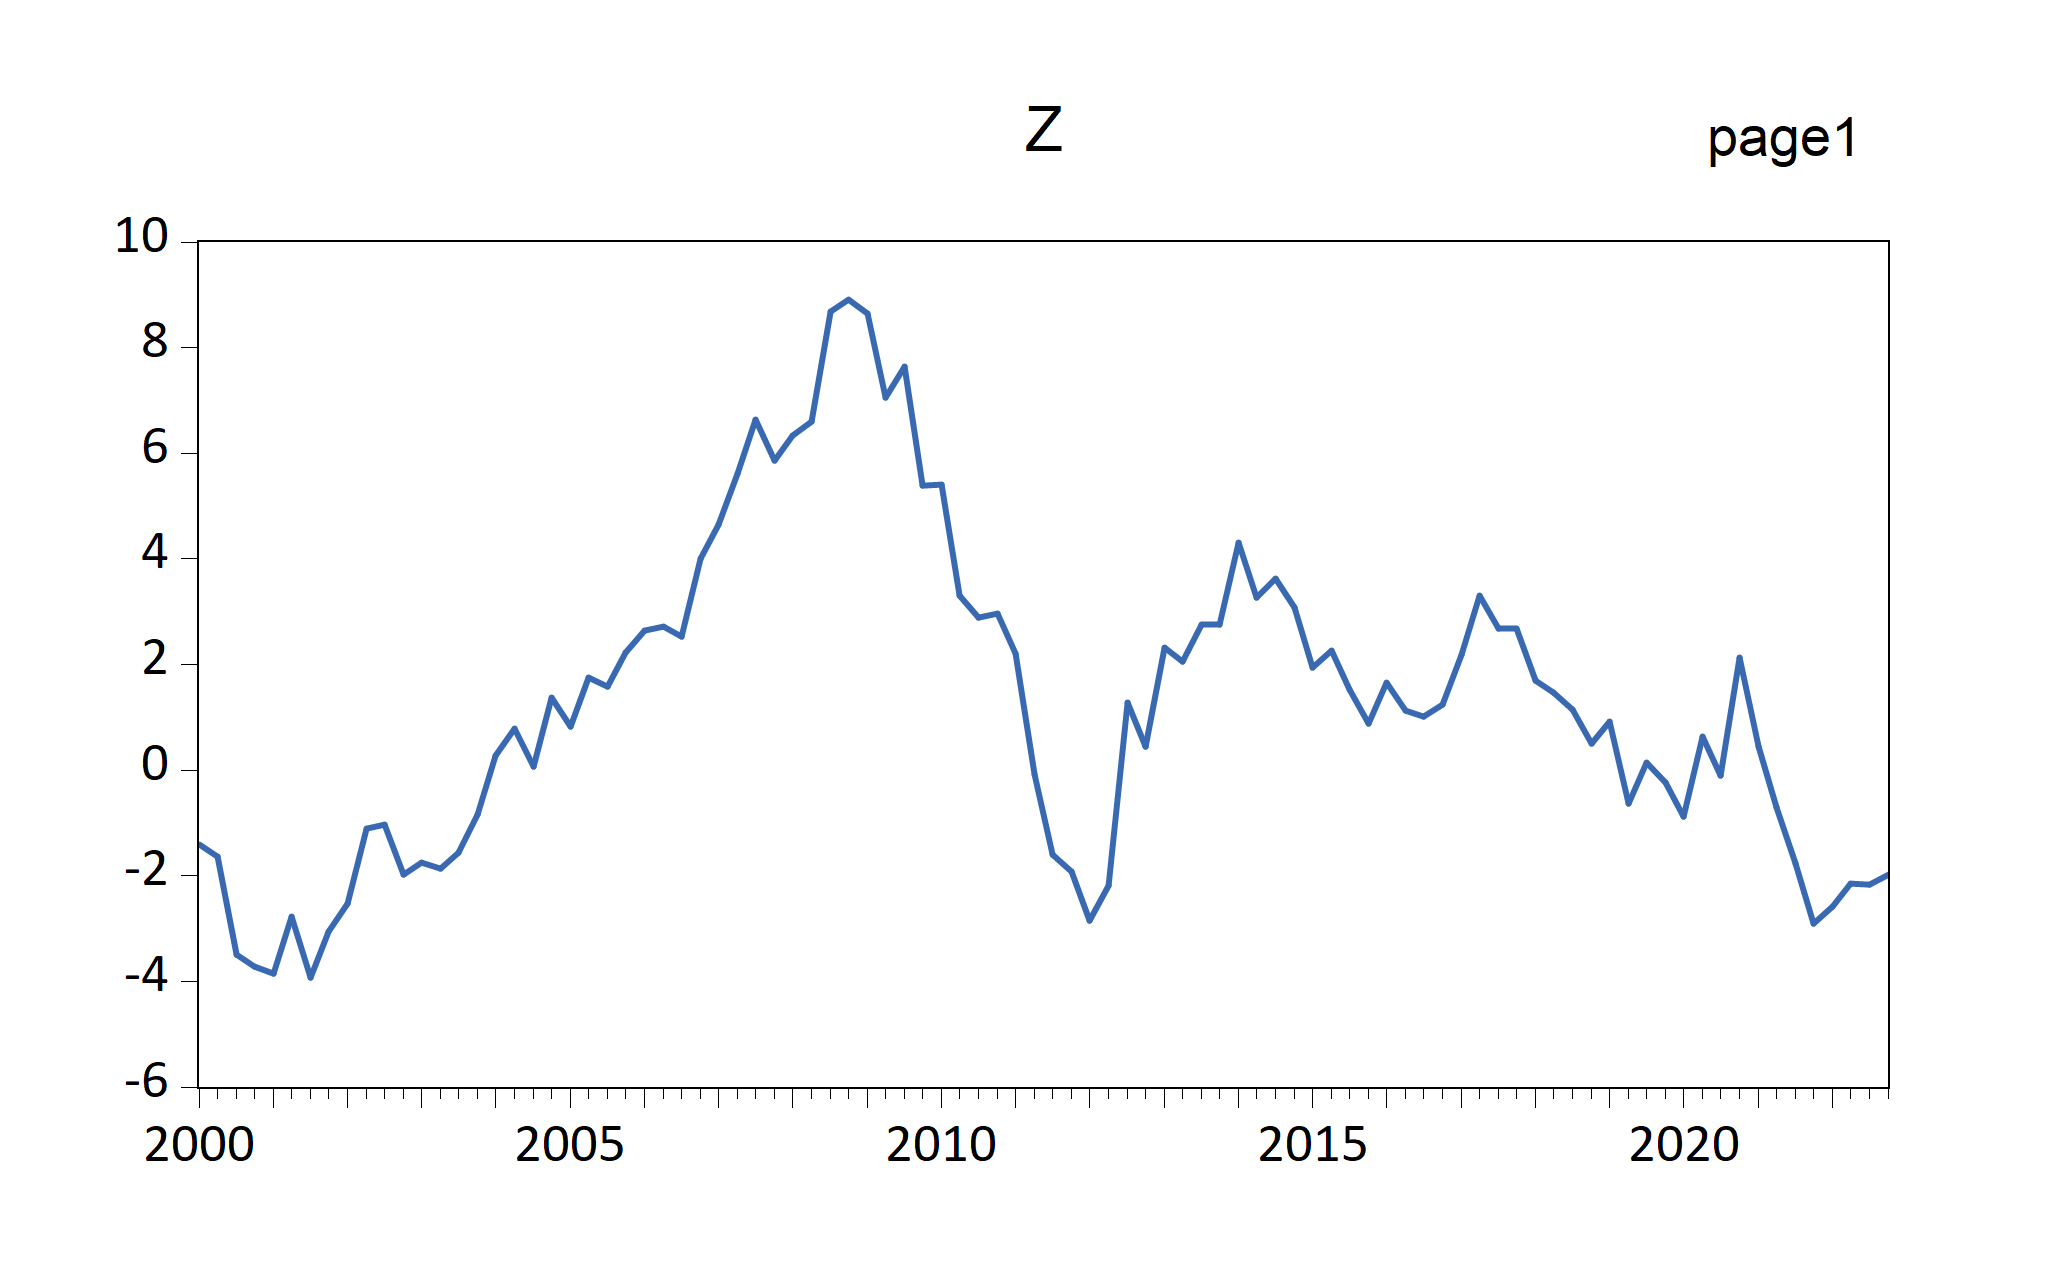
\includegraphics[width=0.32\linewidth,height=0.15\textheight]{figures/eviewsr1page1-graph3} 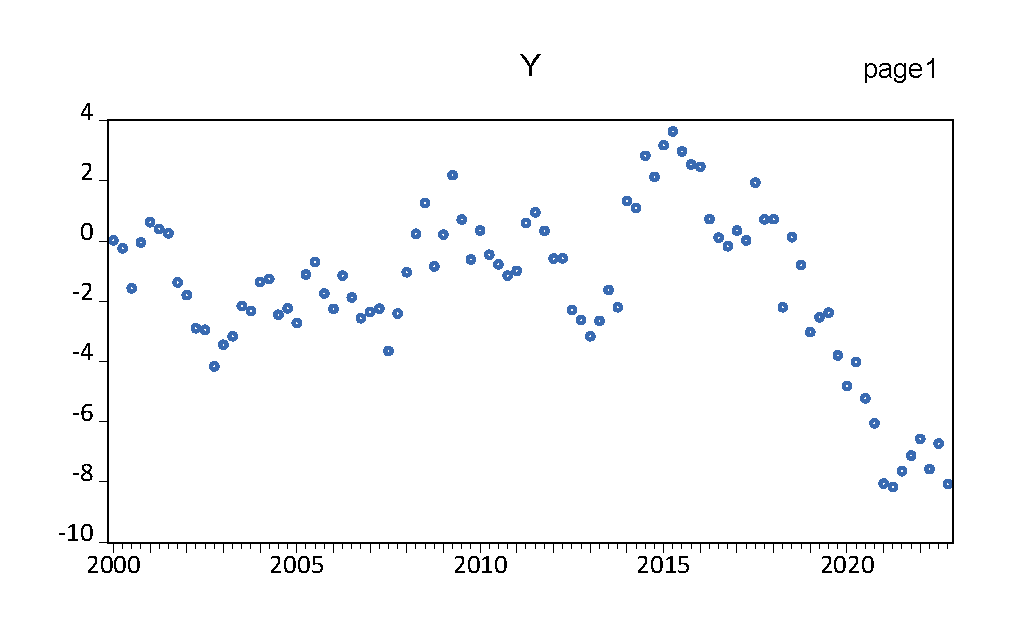
\includegraphics[width=0.32\linewidth,height=0.15\textheight]{figures/eviewsr1page1-graph2} 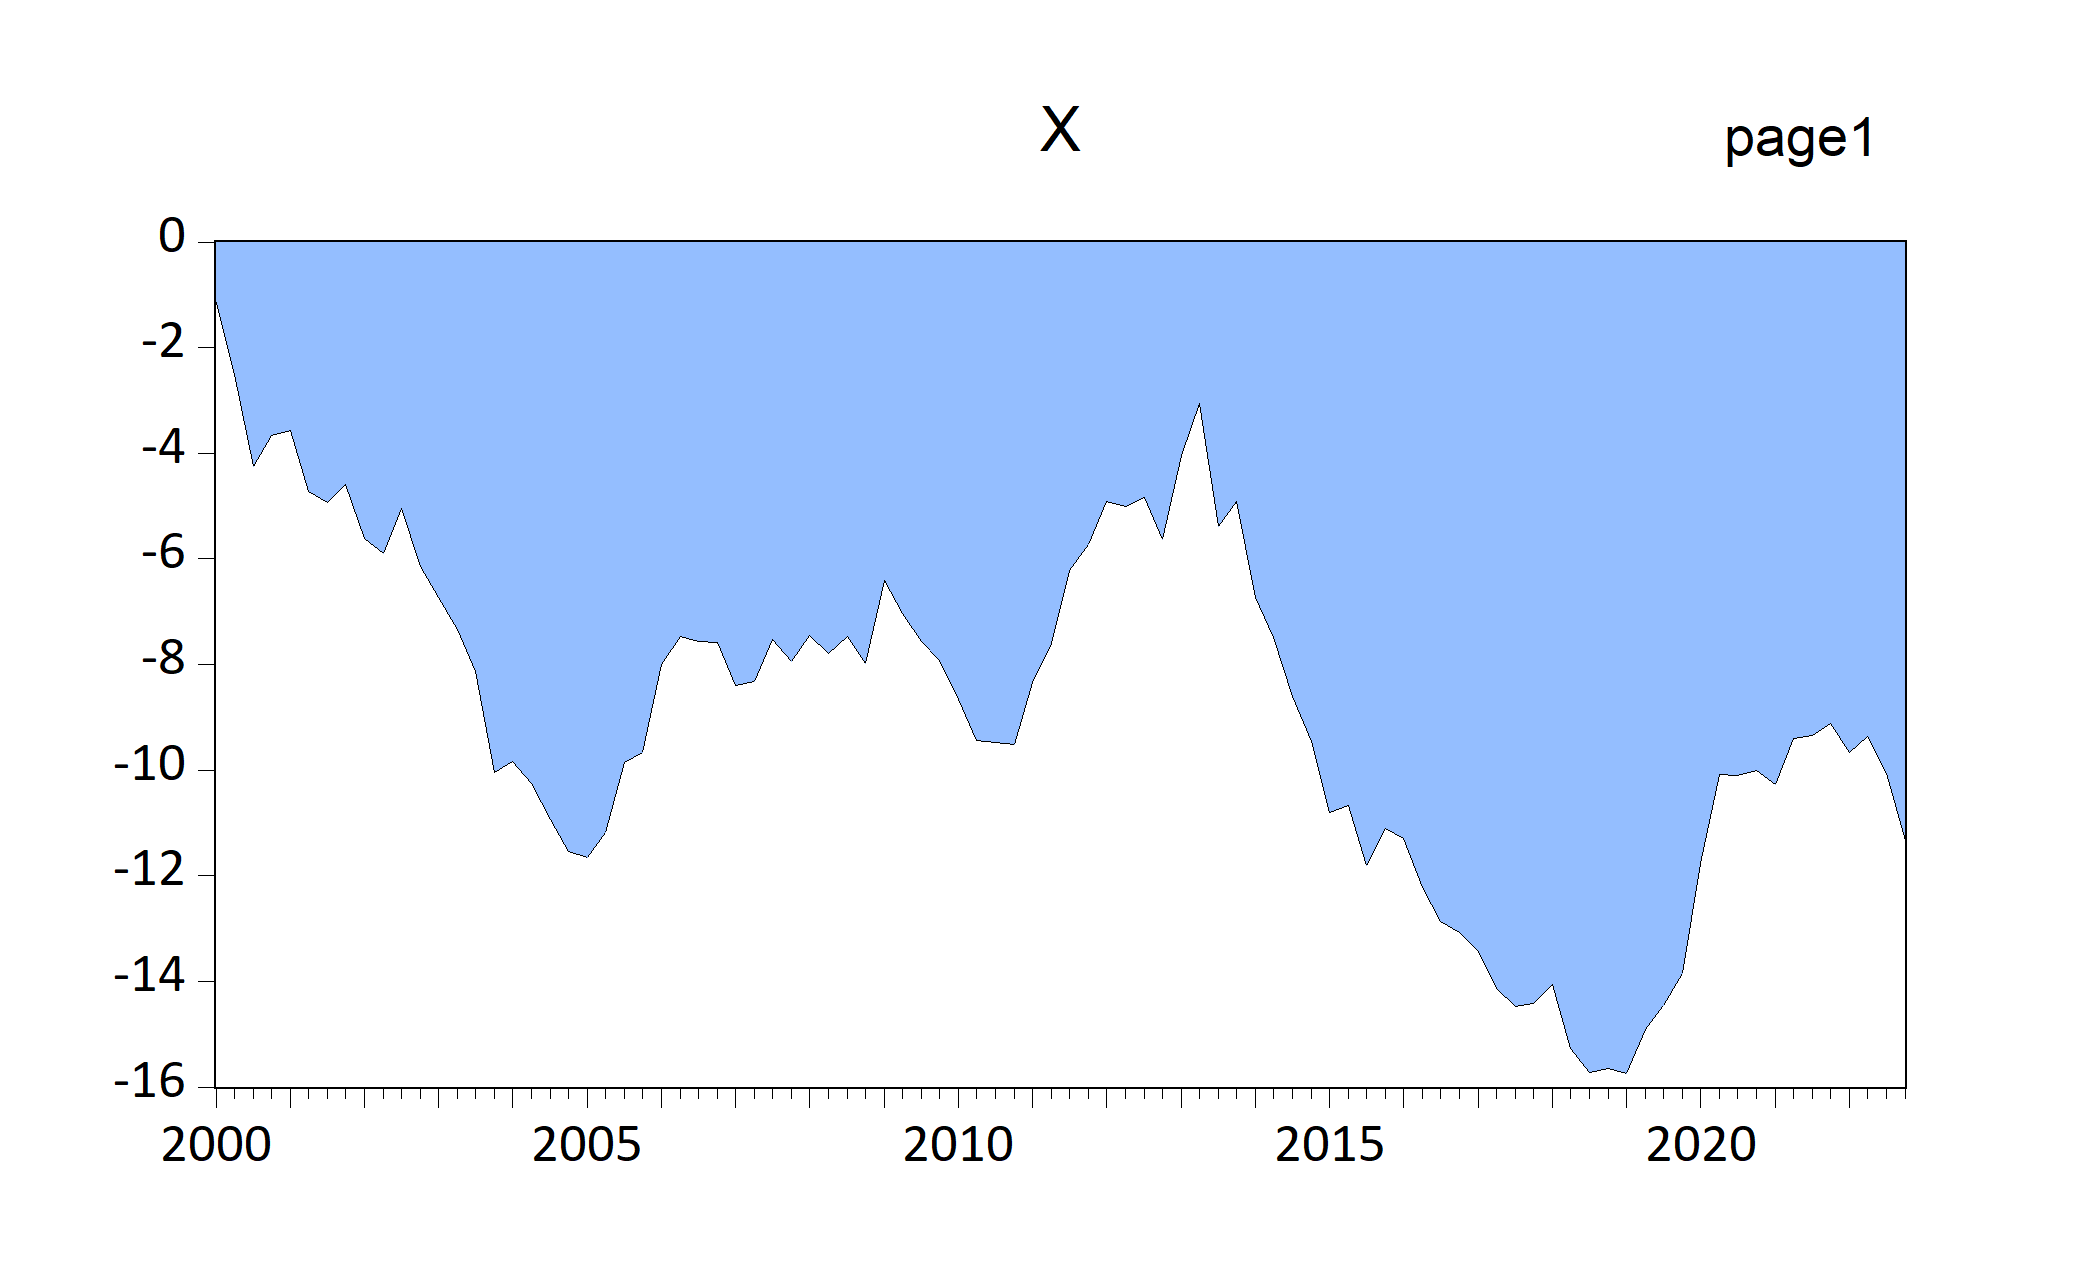
\includegraphics[width=0.32\linewidth,height=0.15\textheight]{figures/eviewsr1page1-graph1} 

}

\caption{EViews graphs automatically imported by EViews chunk (fig-EviewsR2)}\label{fig:fig-EviewsR2-1}
\end{figure}

\hypertarget{use-of-graph_procs-chunk-option}{%
\subsection{Use of graph\_procs chunk option}\label{use-of-graph_procs-chunk-option}}

To plot Figure \ref{fig:fig-EviewsR3-1}, include the following arguments in the chunk options:

\begin{itemize}
\item
  \texttt{graph\_procs:\ {[}template\ bokeh,\ setelem(1)\ lcolor(green)\ fillcolor(green){]}}
\item
  \texttt{graph:\ "@asis"}
\item
  \texttt{page:\ eviewsr\ page1}
\end{itemize}

Note that only the graph objects from pages \texttt{EviewsR} and \texttt{page1} are included.

\begin{figure}

{\centering 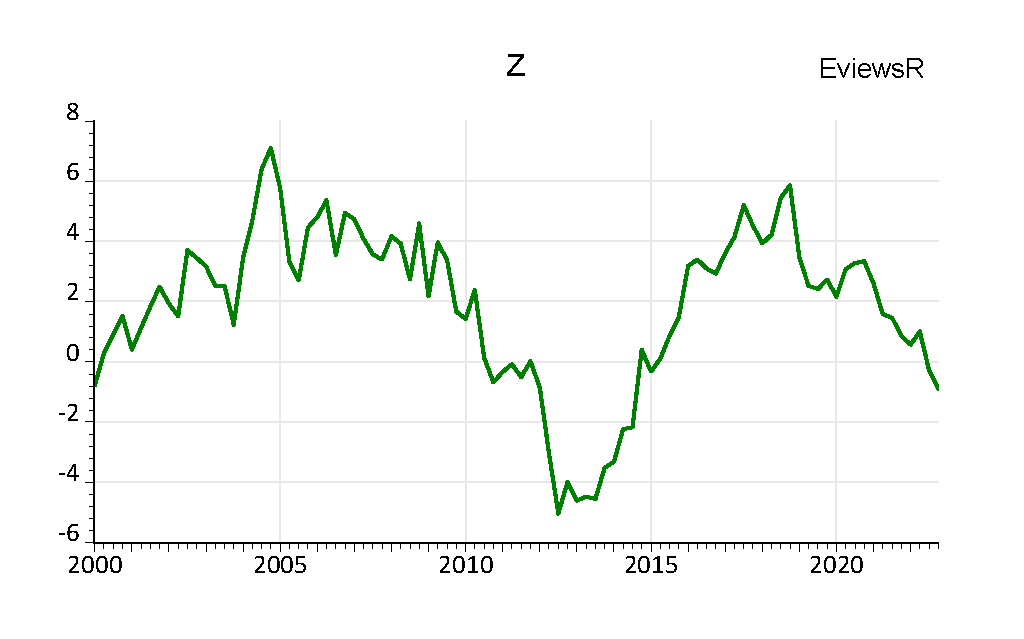
\includegraphics[width=0.32\linewidth,height=0.15\textheight]{figures/eviewsr3-eviewsr-graph3} 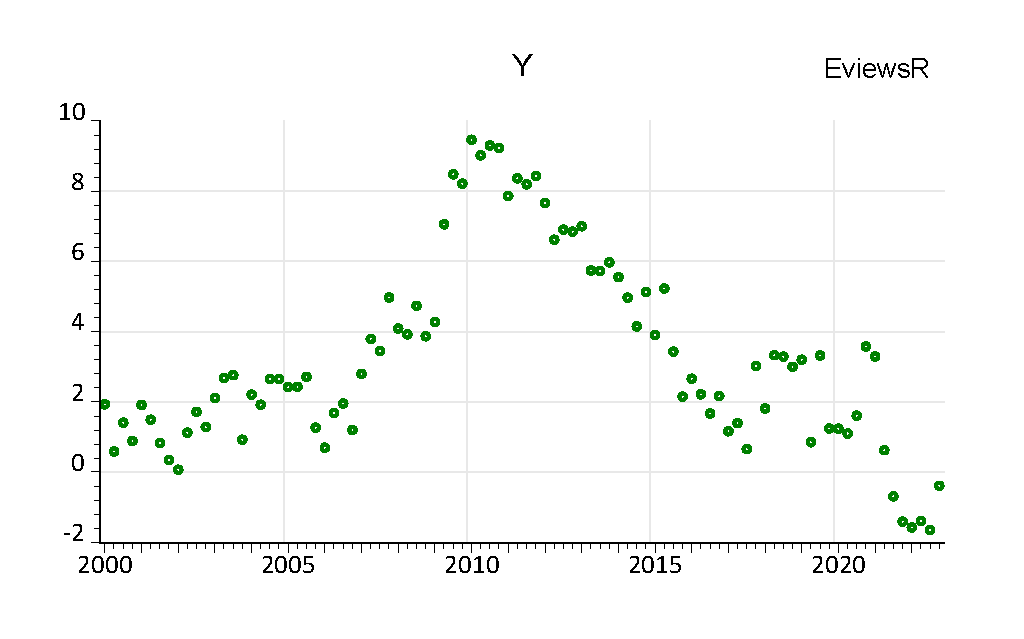
\includegraphics[width=0.32\linewidth,height=0.15\textheight]{figures/eviewsr3-eviewsr-graph2} 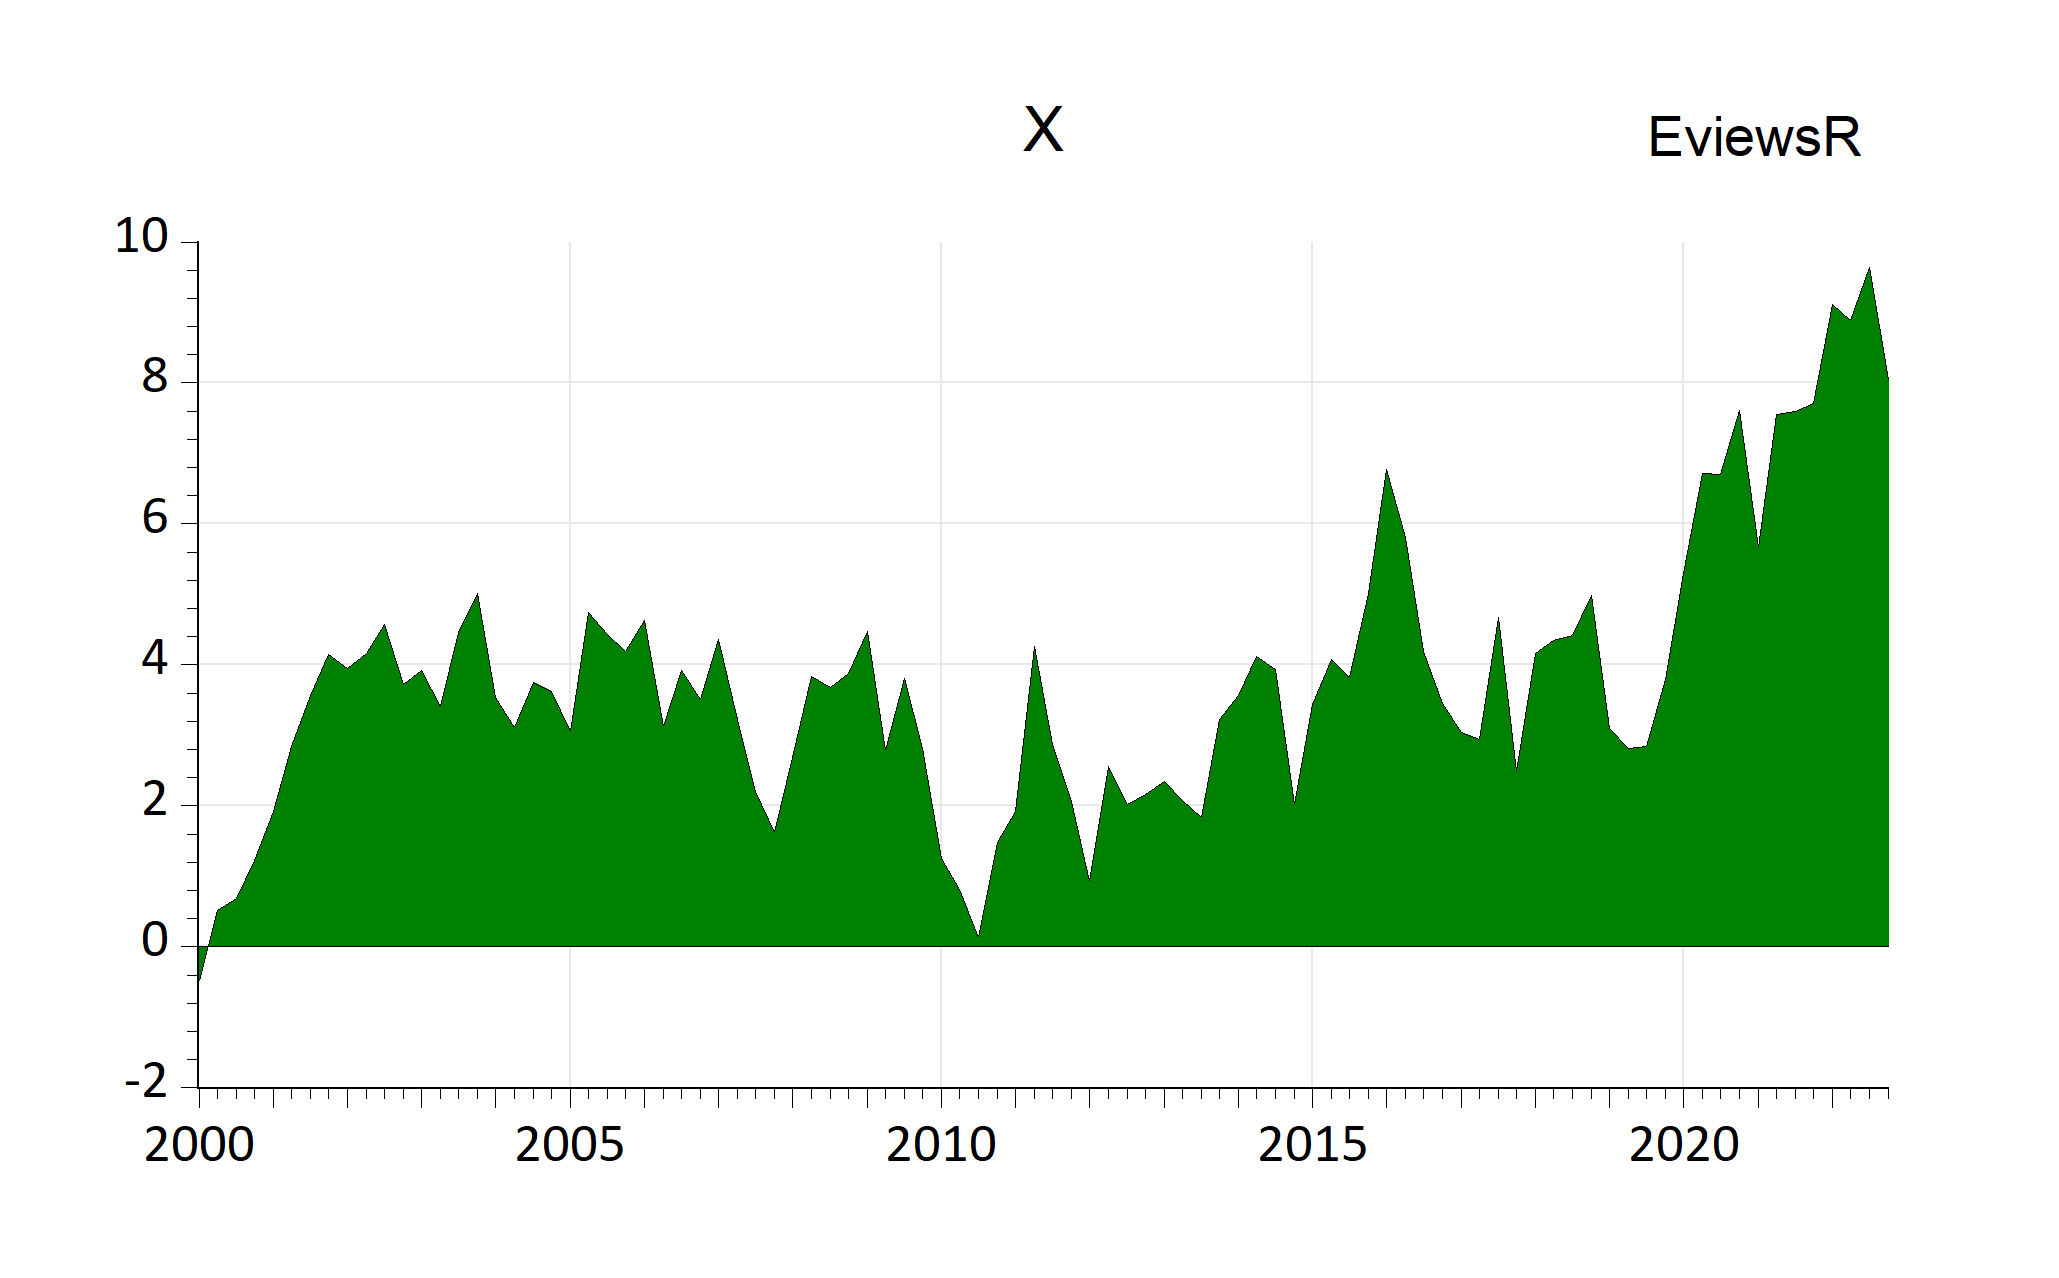
\includegraphics[width=0.32\linewidth,height=0.15\textheight]{figures/eviewsr3-eviewsr-graph1} 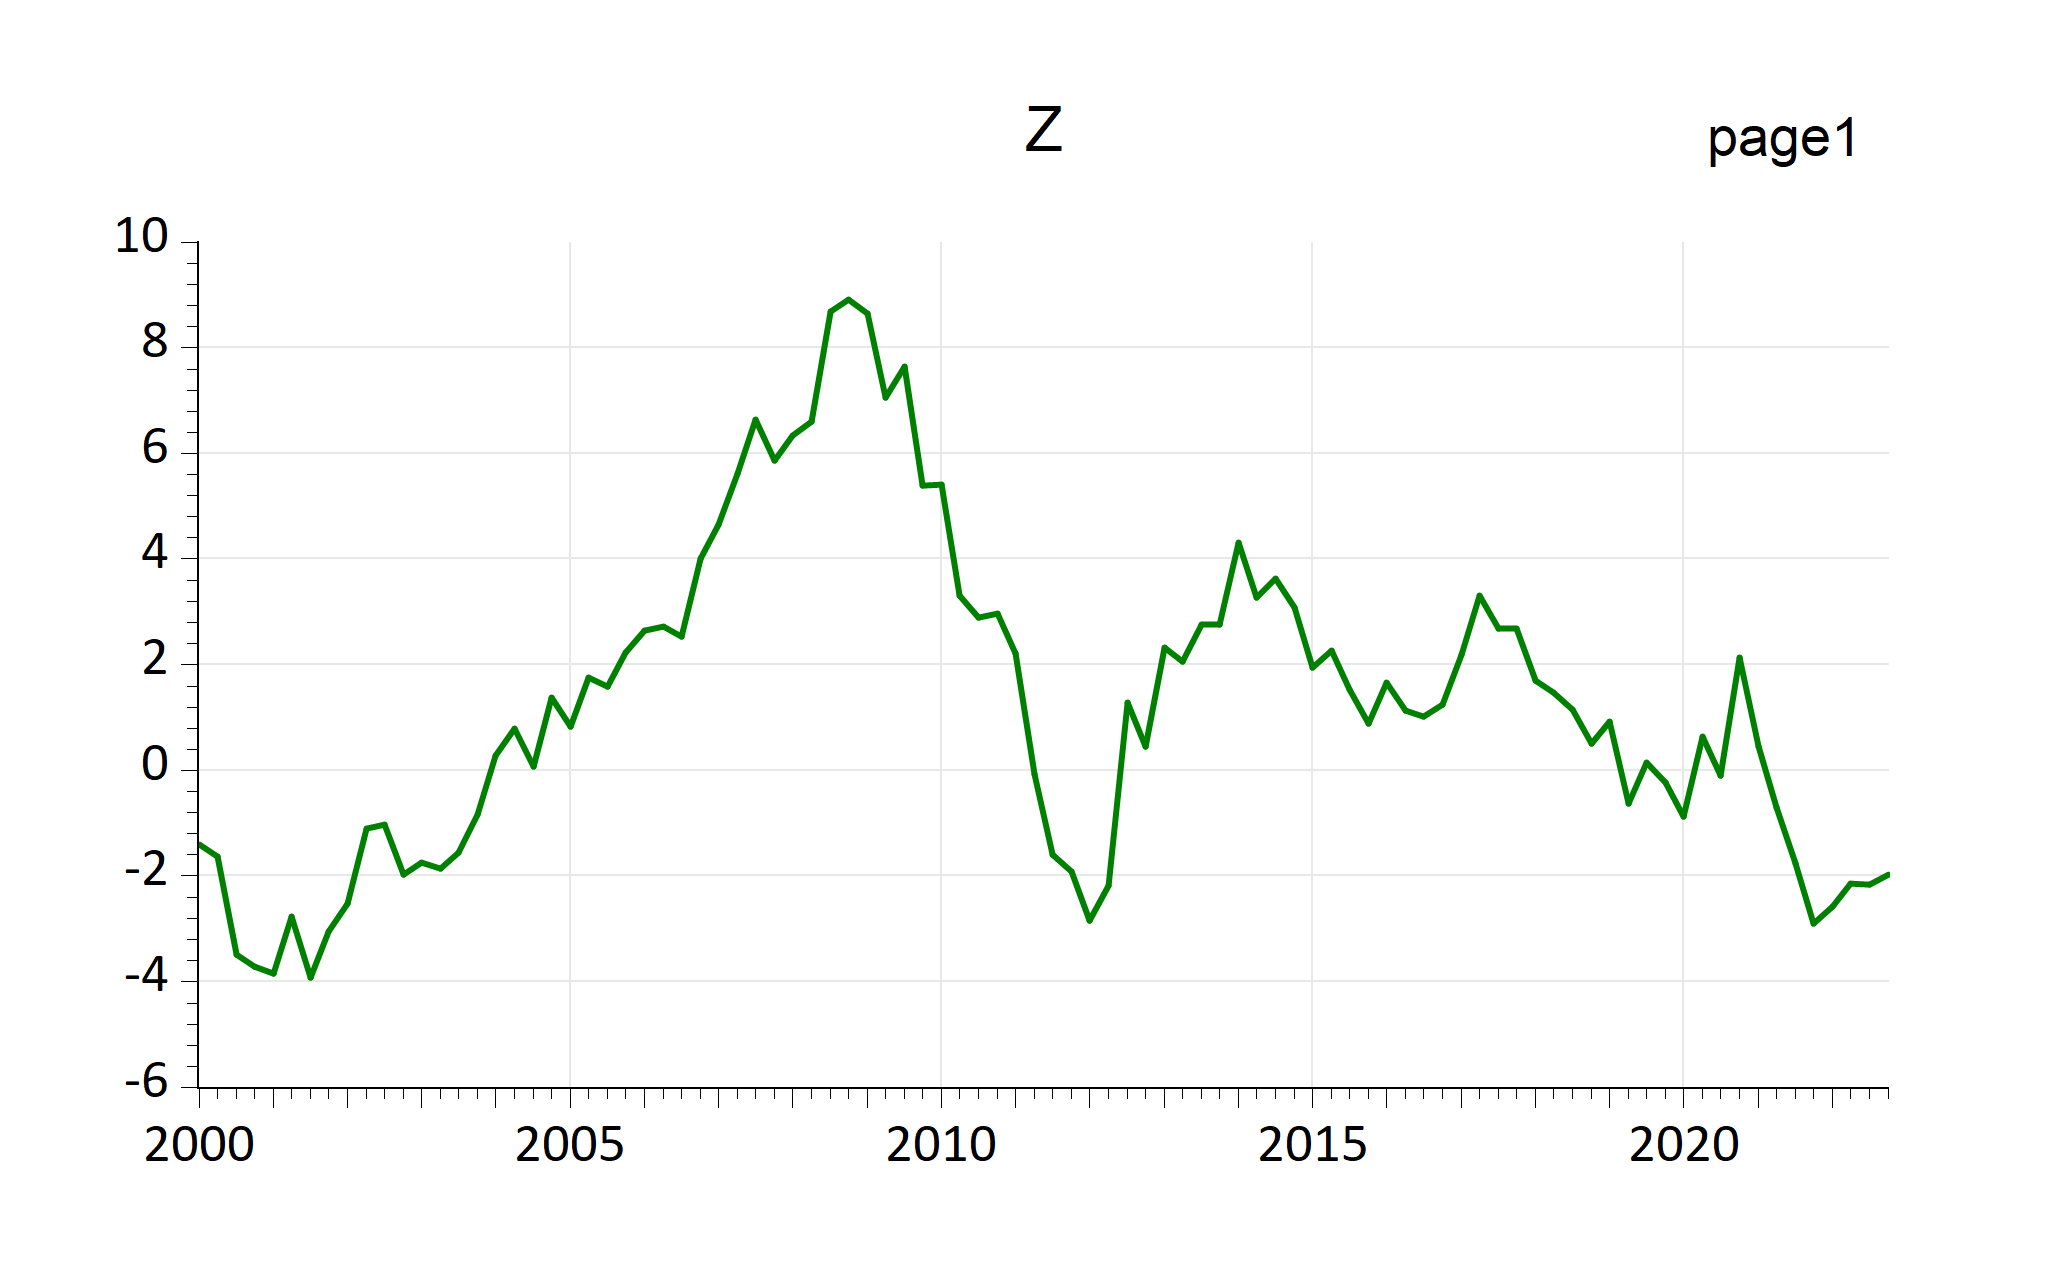
\includegraphics[width=0.32\linewidth,height=0.15\textheight]{figures/eviewsr3-page1-graph3} 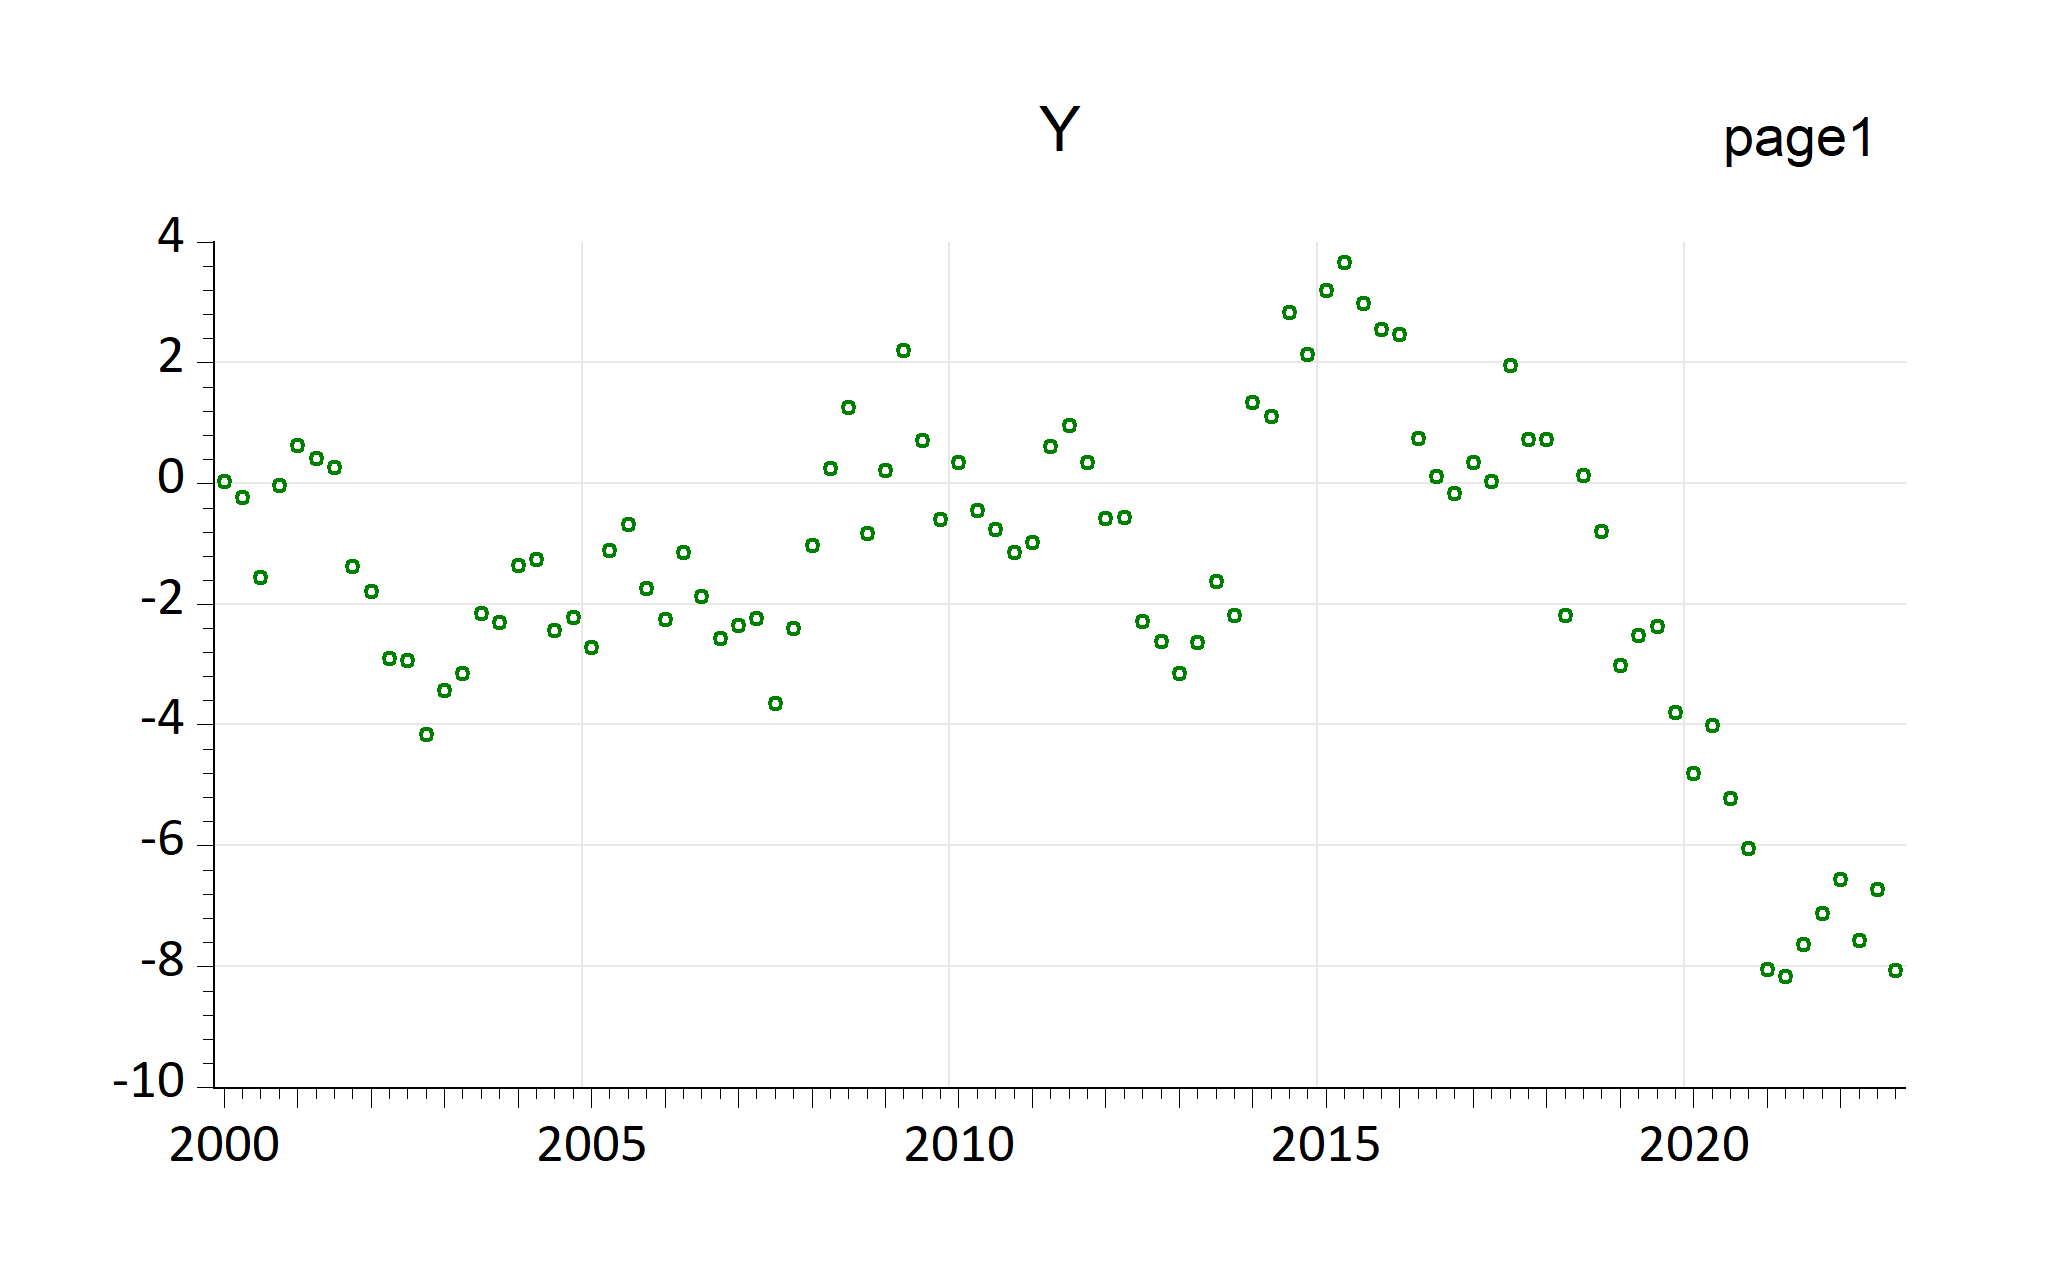
\includegraphics[width=0.32\linewidth,height=0.15\textheight]{figures/eviewsr3-page1-graph2} 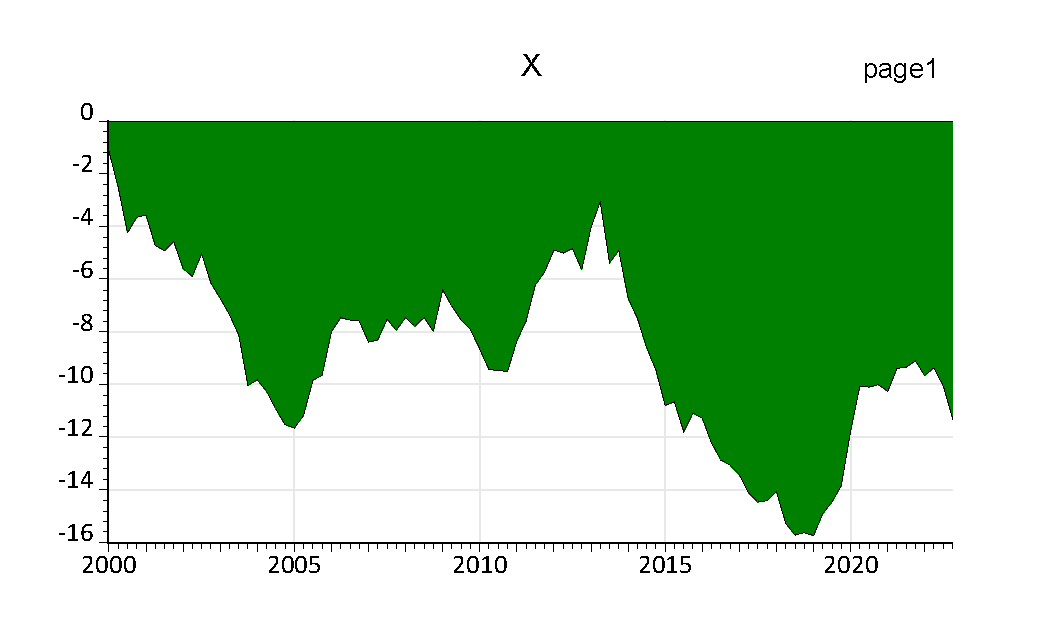
\includegraphics[width=0.32\linewidth,height=0.15\textheight]{figures/eviewsr3-page1-graph1} 

}

\caption{EViews graphs automatically imported by EViews chunk (fig-EviewsR3)}\label{fig:fig-EviewsR3-1}
\end{figure}

\hypertarget{importing-only-the-first-graph}{%
\subsection{Importing only the first graph}\label{importing-only-the-first-graph}}

To plot only the first graph object from each of the EViews pages, after all the graph objects on each page are arranged in ascending order. Therefore only a combination of \texttt{graph1} object from each of the pages is plotted as shown in Figure \ref{fig:fig-EviewsR4-1}:

\begin{itemize}
\item
  \texttt{graph\_procs:\ {[}template\ modern,datelabel\ format("YYYY"),setelem(1)\ fillcolor(red){]}}
\item
  \texttt{graph:\ "@first"}
\end{itemize}

\begin{figure}

{\centering 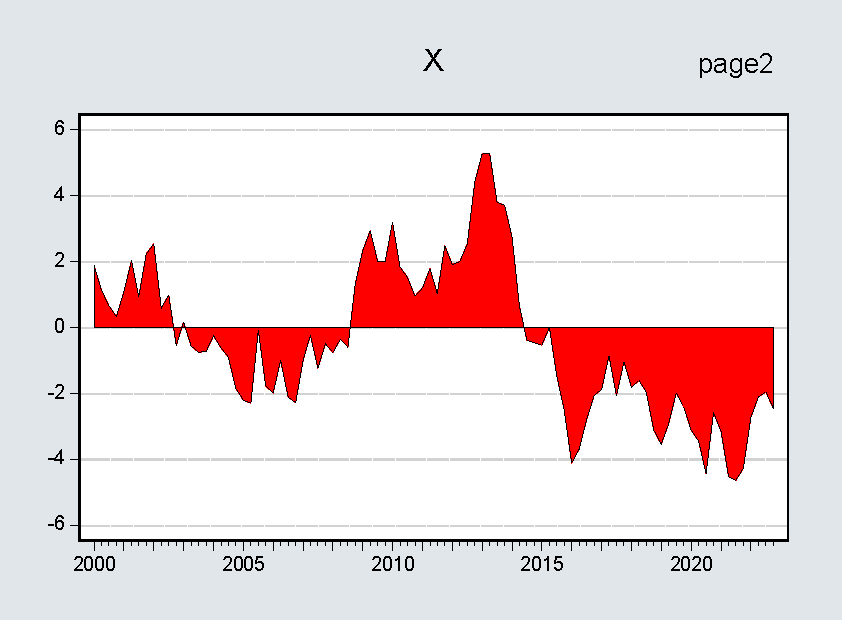
\includegraphics[width=0.32\linewidth,height=0.15\textheight]{figures/eviewsr4page2-graph1} 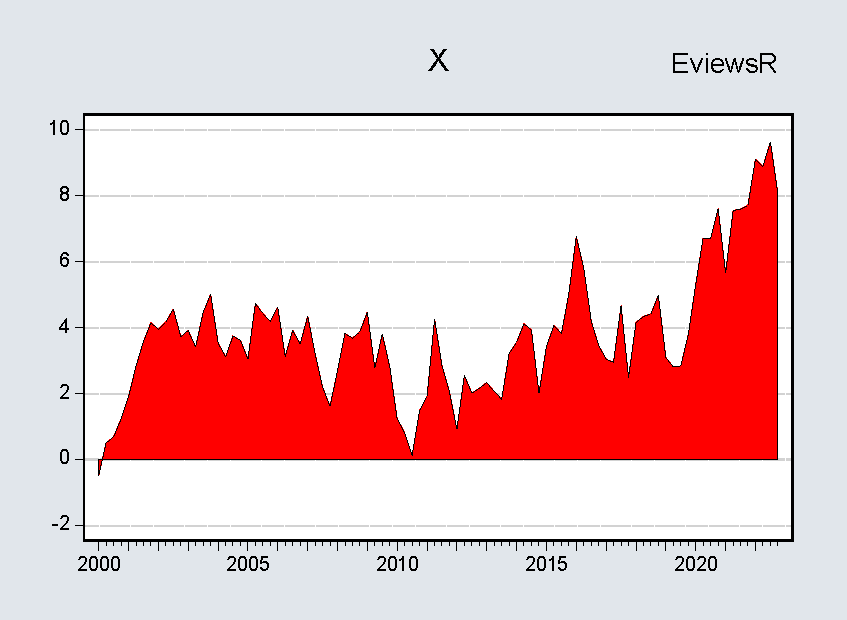
\includegraphics[width=0.32\linewidth,height=0.15\textheight]{figures/eviewsr4eviewsr-graph1} 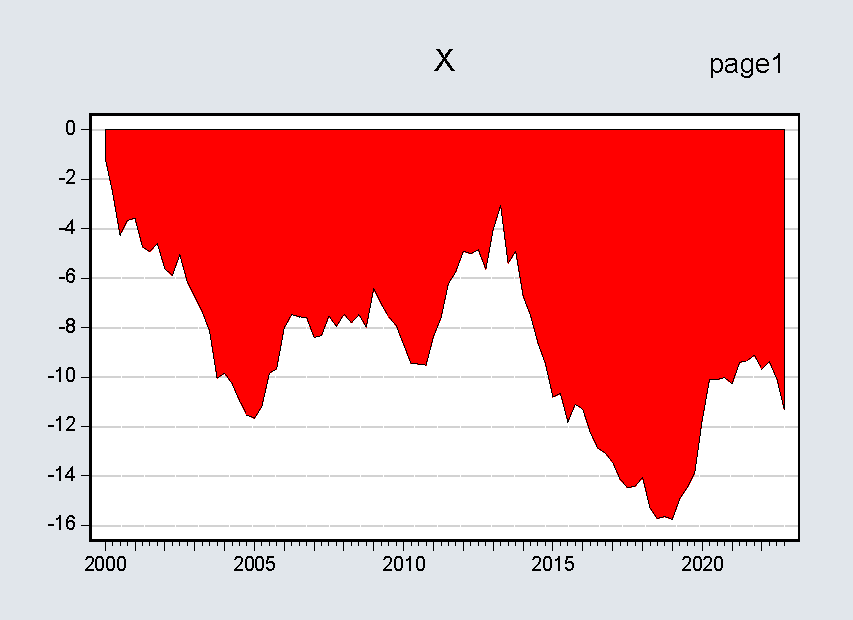
\includegraphics[width=0.32\linewidth,height=0.15\textheight]{figures/eviewsr4page1-graph1} 

}

\caption{Importing only the first EViews graphs by EViews chunk (fig-EviewsR4)}\label{fig:fig-EviewsR4-1}
\end{figure}

\hypertarget{importing-only-the-last-graph}{%
\subsection{Importing only the last graph}\label{importing-only-the-last-graph}}

The chunk option \texttt{graph:\ "@last"} is the direct opposite of the \texttt{graph:\ "\ @first"} as it considers the last graph object only.

\begin{itemize}
\tightlist
\item
  \texttt{graph:\ "@last"}
\end{itemize}

\hypertarget{importing-only-graphs-selected-by-index}{%
\subsection{Importing only graphs selected by index}\label{importing-only-graphs-selected-by-index}}

We modify the chunk options as follows to ensure that only the second, fifth and eighth graph objects across all pages, are included in the output. Therefore only \texttt{graph2} object from each of the pages is considered.

\begin{itemize}
\tightlist
\item
  \texttt{graph:\ {[}2,5,8{]}}
\end{itemize}

\hypertarget{importing-graphs-in-ascendingdescending-order}{%
\subsection{Importing graphs in ascending/descending order}\label{importing-graphs-in-ascendingdescending-order}}

We arranges all the graph objects across all the pages in ascending order by setting:

\begin{itemize}
\tightlist
\item
  \texttt{graph:\ "@asc"}
\end{itemize}

We can also import the graphs in descending order by:

\begin{itemize}
\tightlist
\item
  \texttt{graph:\ "@desc"}
\end{itemize}

\hypertarget{sec-base}{%
\section{EviewsR: base R functions}\label{sec-base}}

We understand that not everyone uses R Markdown or Quarto. Moreover, some EViews computations may take long time to complete, in which case it will be better to work with the existing workfile. For these reasons, we create a number of R functions that can be used to communicate with EViews from R. The functions include:

To work with EViews, a workfile and a workfile page are required, therefore we add \texttt{wf} (workfile) and \texttt{page} (workfile page) arguments for each function. These functions are explained as follows:

\hypertarget{the-create_object-function.}{%
\subsection{The create\_object() function.}\label{the-create_object-function.}}

The function \texttt{create\_object()} can be used to create an EViews object in the existing EViews workfile. We can use the EViews workfile (\texttt{EviewsR.wf1}) created by the EViews chunk in Section \ref{sec-document}. The complete EViews syntax for an object command has the form:

\begin{verbatim}
EViews> action(action_opt) object_name.view_or_proc(options_list) arg_list

EViews> object_type(options) object_name[=expression]
\end{verbatim}

Where \texttt{action} can be one of the four EViews commands (\texttt{do}, \texttt{freeze}, \texttt{print}, \texttt{show}); \texttt{action\_opt} modifies the default behaviour of the \texttt{action}; \texttt{object\_name} is any arbitrary character string to represent the name of the EViews object to be acted upon; \texttt{view\_or\_proc} stands for the EViews object's view or procedure to be performed; \texttt{options\_list} is the option for the \texttt{view\_or\_proc}; \texttt{arg\_list} stands for the EViews view or procedure arguments.

To create an equation object \texttt{eviews\_equation} as an \texttt{ar(1)} process on \texttt{EviewR1} page of \texttt{EviewsR.wf1} workfile, we can use the following EViews code:

\begin{verbatim}
EViews> wfopen EviewsR_files/EviewsR
EViews> pageselect EviewsR1
EViews> equation eviews_equation.ls y ar(1)
EViews> wfsave EviewsR_files/EviewsR
\end{verbatim}

The above can be translated into base R function as:

\begin{verbatim}
R> create_object(wf = "EviewsR_files/EviewsR", page = "EviewsR1",
+     action = "equation", object_name = "eviews_equation", view_or_proc = "ls",
+     arg_list = "y ar(1)")
\end{verbatim}

To create a series object \texttt{series1} and assign it to the square of \(y\) series on \texttt{EviewsR2} page of \texttt{EviewsR.wf1} workfile:

\begin{verbatim}
EViews> wfopen EviewsR_files/EviewsR
EViews> pageselect EviewsR2
EViews> series series1=y^2
EViews> wfsave EviewsR_files/EviewsR
\end{verbatim}

\begin{verbatim}
R> create_object(wf = "EviewsR_files/EviewsR", page = "EviewsR2",
+     object_type = "series", object_name = "series1", expression = "y^2")
\end{verbatim}

\hypertarget{sec-figures}{%
\subsection{The eviews\_graph() function}\label{sec-figures}}

EViews graph can be included in an R Markdown or Quarto document by \texttt{eviews\_graph()} function. This function is a blend of EViews \texttt{freeze}, \texttt{graph} and \texttt{save} commands. The following are the EViews syntaxes:

\begin{verbatim}
EViews> freeze(options, name) object_name.view_command
EViews> graph graph_name.graph_command(options) arg1 [arg2 arg3 ...]
EViews> graph_name.save(options) [path\]file_name
\end{verbatim}

The first and second syntaxes can be merged to produce another syntax which we use to create the \texttt{eviews\_graph()} function. So the new syntax is:

\begin{verbatim}
EViews> freeze(options, name) object_name.graph_command(options)
\end{verbatim}

Each of the \texttt{freeze}, \texttt{graph\_command} and \texttt{save} commands has an \texttt{options} keyword. We use \texttt{mode} for \texttt{freeze} command options, \texttt{graph\_options} for \texttt{graph\_command} command options, and \texttt{save\_options} for \texttt{save} command options. Check EViews manual for all the available options for these commands.

The \texttt{series} argument can be the names of EViews series objects or an R dataframe. If \texttt{series} is a set of EViews series objects, \texttt{wf} and \texttt{page} need to be specified. If \texttt{series} is an R dataframe, \texttt{wf} and \texttt{page} are optional.

To create figures of series objects x and y saved on \texttt{EviewsR} page of the \texttt{EviewsR.wf1} workfile:

\begin{verbatim}
EViews> wfopen EviewsR_files/eviewsr
EViews> pageselect eviewsr
EViews> freeze(eviewsGraph_x,mode=overwrite) x.line
EViews> freeze(eviewsGraph_y,mode=overwrite) y.line
EViews> for %y eviewsGraph_x eviewsGraph_y
EViews> {%y}.axis(l) font(Calibri,14,-b,-i,-u,-s)
EViews> {%y}.axis(r) font(Calibri,14,-b,-i,-u,-s)
EViews> {%y}.axis(b) font(Calibri,14,-b,-i,-u,-s)
EViews> {%y}.axis(t) font(Calibri,14,-b,-i,-u,-s)
EViews> {%y}.legend columns(5) inbox position(BOTCENTER) font(Calibri,12,-b,-i,-u,-s)
EViews> {%y}.options antialias(on)
EViews> {%y}.options size(6,3)
EViews> {%y}.options -background frameaxes(all) framewidth(0.5)
EViews> {%y}.setelem(1) linecolor(@rgb(57,106,177)) linewidth(1.5)
EViews> {%y}.setfont legend(Calibri,12,-b,-i,-u,-s) text(Calibri,14,-b,-i,-u,-s) 
EViews> {%y}.setfont obs(Calibri,14,-b,-i,-u,-s)
EViews> {%y}.textdefault font(Calibri,14,-b,-i,-u,-s)
EViews> {%y}.save(t=pdf) {%y} 
EViews> next
\end{verbatim}

Note that the EViews \texttt{for\ loop} in the code above contains the default values of EViews graph procedures provided by \CRANpkg{EviewsR} package. It can be found in the \texttt{eviews\_graph()} function's skeleton defined as \texttt{graphicsDefault}. We will avoid repeating the default values and use `insert default values' instead. \color{black} These default values can be modified or replaced entirely by using \texttt{graph\_procs} argument. For example the line colour of the first graph element is blue by default. This can be changed to red by setting \texttt{graph\_procs="setelem(1)\ linecolor(red)"}, which overwrites the default ``\texttt{setelem(1)\ linecolor(@rgb(57,106,177))}''. We can also overwrite the default behaviour by setting any available EViews templates, for example \texttt{graph\_grocs="template\ defaults"}, which resets the graph objects to EViews global graphics defaults.

The EViews code above can be easily written as an R chunk to produce Figure \ref{fig:fig-eviewsGraph} as follows:

\begin{verbatim}
```{r}  
#| label: fig-eviewsGraph
#| fig.cap: EviewsR example figure using \LaTeX{} subfig package
#| fig.show: hold
#| out.width: 45%
#| out.height: 15%
#| eval: TRUE

eviews_graph(series="x y",wf="EviewsR_files/EviewsR",page = "EviewsR",save_options="t=pdf")

```
\end{verbatim}

\begin{figure}

{\centering 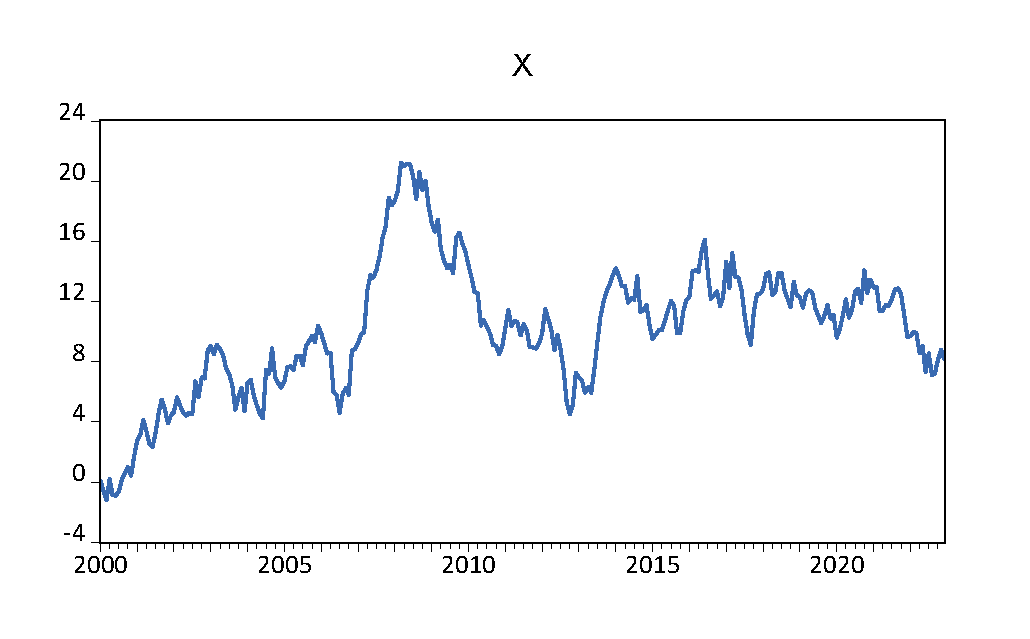
\includegraphics[width=0.45\linewidth,height=0.15\textheight]{figures/eviewsgraph-eviewsr-x} 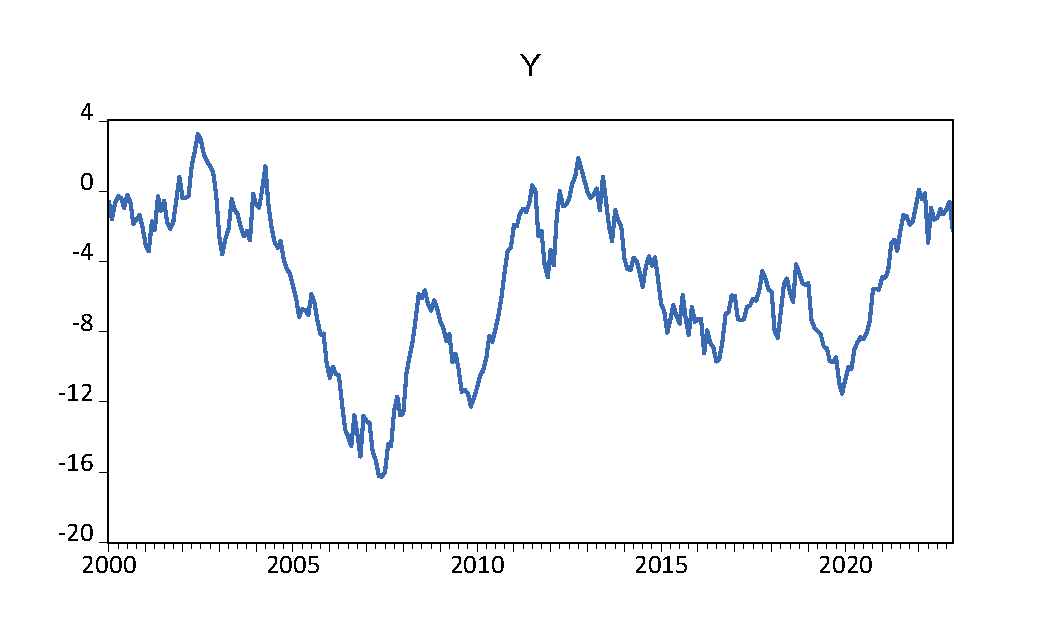
\includegraphics[width=0.45\linewidth,height=0.15\textheight]{figures/eviewsgraph-eviewsr-y} 

}

\caption{EviewsR example figure using \LaTeX{} subfig package}\label{fig:fig-eviewsGraph}
\end{figure}

To produce EViews graphs aligned in two columns, as in Figure \ref{fig:fig-eviewsGraph1}, from an R dataframe named \texttt{EviewsRDataFrame}:

\begin{itemize}
\tightlist
\item
  Use R's \texttt{write.csv()} function to write the dataframe as a CSV file.
\end{itemize}

\begin{verbatim}
R> write.csv(EviewsRDataFrame, "csvFile.csv", row.names = FALSE)
\end{verbatim}

\begin{itemize}
\tightlist
\item
  Use EViews to import the \texttt{csvFile.csv}, then create and save the graphs on disk:
\end{itemize}

\begin{verbatim}
EViews> import csvFile.csv @freq m start_date=1990
EViews> group some_group x y
EViews> freeze(eviewsGraph1_xy,mode=overwrite) some_group.line(m)
                    insert default values
EViews> eviewsGraph1_xy.axis(b) angle(45) font(b)
EViews> eviewsGraph1_xy.save(t=png,d=300) eviewsGraph1_xy
\end{verbatim}

\begin{itemize}
\tightlist
\item
  Use \CRANpkg{knitr}'s \texttt{include\_graphics()} function to import the graph into the R Markdown or Quarto document.
\end{itemize}

The values provided by \texttt{graph\_procs} argument are appended to the graph's default values. Therefore, \texttt{graph\_procs} overwrites the existing default value of the EViews graph procedures.

We use the following options to modify the figure:

\begin{itemize}
\tightlist
\item
  \texttt{group=TRUE}
\item
  \texttt{graph\_options="m"}
\item
  \texttt{graph\_procs="axis(b)\ angle(45)\ font(b)"}
\end{itemize}

\begin{verbatim}
```{r} 
#| label: fig-eviewsGraph1
#| fig.cap: "EViews graph from dataframe (chunk: fig-eviewsGraph1)"
#| out.width: 90%
#| out.height: 15%
#| eval: true

eviews_graph(series=EviewsRDataFrame,start_date = "1990",group=TRUE,
graph_options="m",graph_procs="axis(b) angle(45) font(b)")
```
\end{verbatim}

\begin{figure}

{\centering 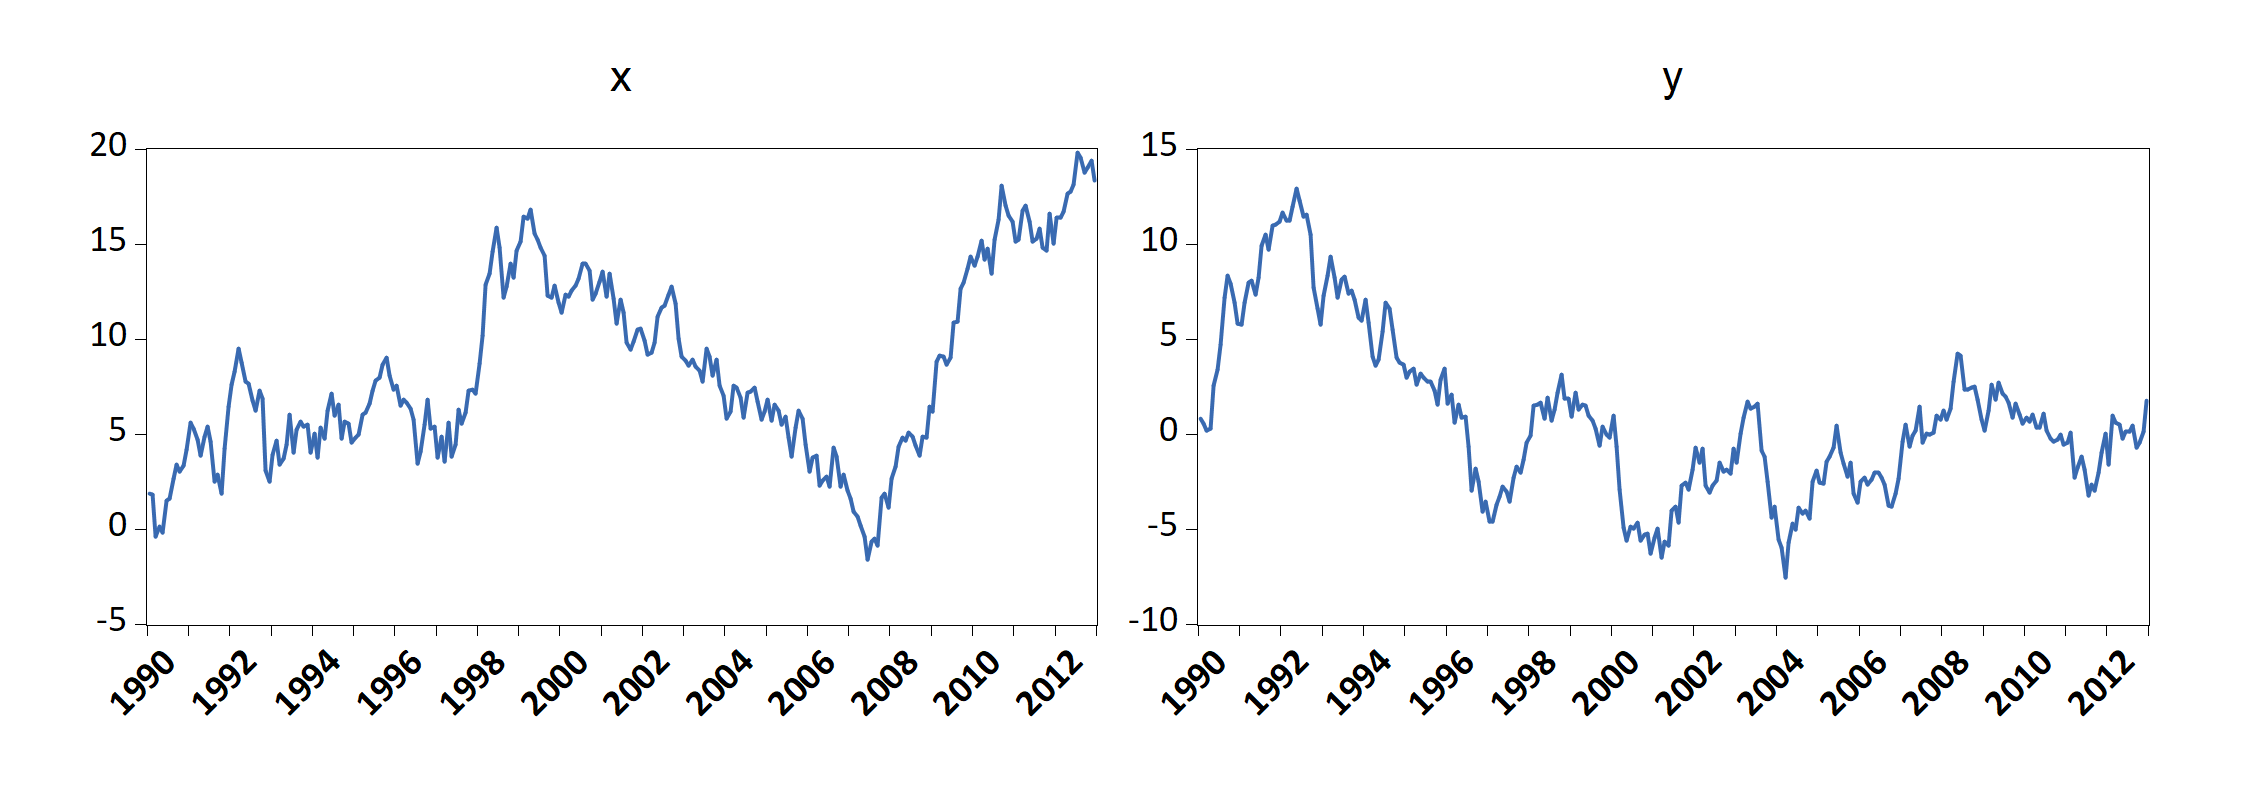
\includegraphics[width=0.9\linewidth,height=0.15\textheight]{figures/eviewsgraph1-eviewsgraph1-xy} 

}

\caption{EViews graph from dataframe (chunk: fig-eviewsGraph1)}\label{fig:fig-eviewsGraph1}
\end{figure}

To create a scatterplot along with histogram on each axis border using green colour (\#008753 hex code):

\begin{verbatim}
EViews> wfopen EviewsR_files/eviewsr
EViews> pageselect eviewsr
EViews> group some_group x y
EViews> freeze(eviewsGraph2_xy,mode=overwrite) some_group.scat(ab=histogram) linefit()
                    insert default values
EViews> eviewsGraph2_xy.setelem(1) lcolor(@hex(008753))
EViews> eviewsGraph2_xy.save(t=png,d=300) eviewsGraph2_xy
\end{verbatim}

The equivalent R chunk to produce Figure \ref{fig:fig-eviewsGraph2}:

\begin{verbatim}
```{r} 
#| label: fig-eviewsGraph2
#| fig.cap: EViews graph from dataframe  
#| out.width: 90%
#| out.height: 40%
#| eval: TRUE

eviews_graph(series="x y",wf="EviewsR_files/EviewsR",page="EviewsR",
graph_command="scat(ab=histogram) linefit()",group=TRUE,
graph_procs='setelem(1) lcolor(@hex(008753))')
```
\end{verbatim}

\begin{figure}

{\centering 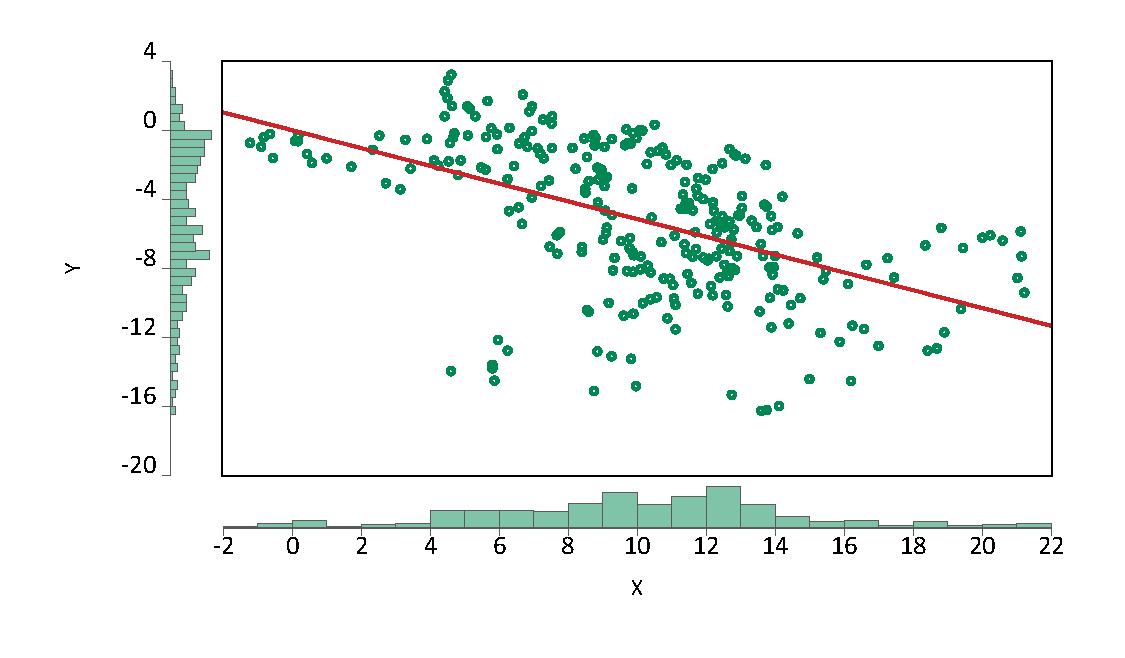
\includegraphics[width=0.9\linewidth,height=0.4\textheight]{figures/eviewsgraph2-eviewsr-xy} 

}

\caption{EViews graph from dataframe (chunk: fig-eviewsGraph2)}\label{fig:fig-eviewsGraph2}
\end{figure}

If we want to plot all the series objects contained in \texttt{EviewsR2} page of \texttt{EviewsR.wf1} workfile that lives in \texttt{EviewsR\_files/} folder, we can simply use:

\begin{verbatim}
R> eviews_graph(wf = "EviewsR_files/EviewsR", page = "EviewsR2")
\end{verbatim}

Note that we have not specified the \texttt{series} argument as \texttt{eviews\_graph()} function is designed to plot all series objects by default. Similarly, we do not need to provide the \texttt{page} argument if we intend to include the graphs of all the series objects from all the pages of the workfile. We can also use any valid EViews wildcard expressions or pattern, such as \texttt{series="x*"}, \texttt{series="???x"} and so on.

To plot two or more line graphs with daily frequency on one frame from a dataframe:

\begin{verbatim}
EViews> import csvFile.csv @freq 7 start_date=2000
EViews> group some_group x y
EViews> freeze(eviewsGraph3_xy,mode=overwrite) some_group.line
                    insert default values
EViews> eviewsGraph3_xy.datelabel format("dd Mon, yyyy")  interval(month,1)
EViews> eviewsGraph3_xy.save(t=png,d=300) eviewsGraph3_xy
\end{verbatim}

Figure \ref{fig:fig-eviewsGraph3} uses the R equivalent of the above EViews code as follows:

\begin{verbatim}
```{r} 
#| label: fig-eviewsGraph3
#| fig.cap: "EViews graph from dataframe (chunk: fig-eviewsGraph3)"
#| out.width: 90%
#| out.height: 40%
#| eval: TRUE

eviews_graph(series=EviewsRDataFrame,frequency="7",start_date = "2000",group = TRUE,
graph_procs='datelabel format("dd Mon, yyyy")  interval(month,1)')
```
\end{verbatim}

\begin{figure}

{\centering 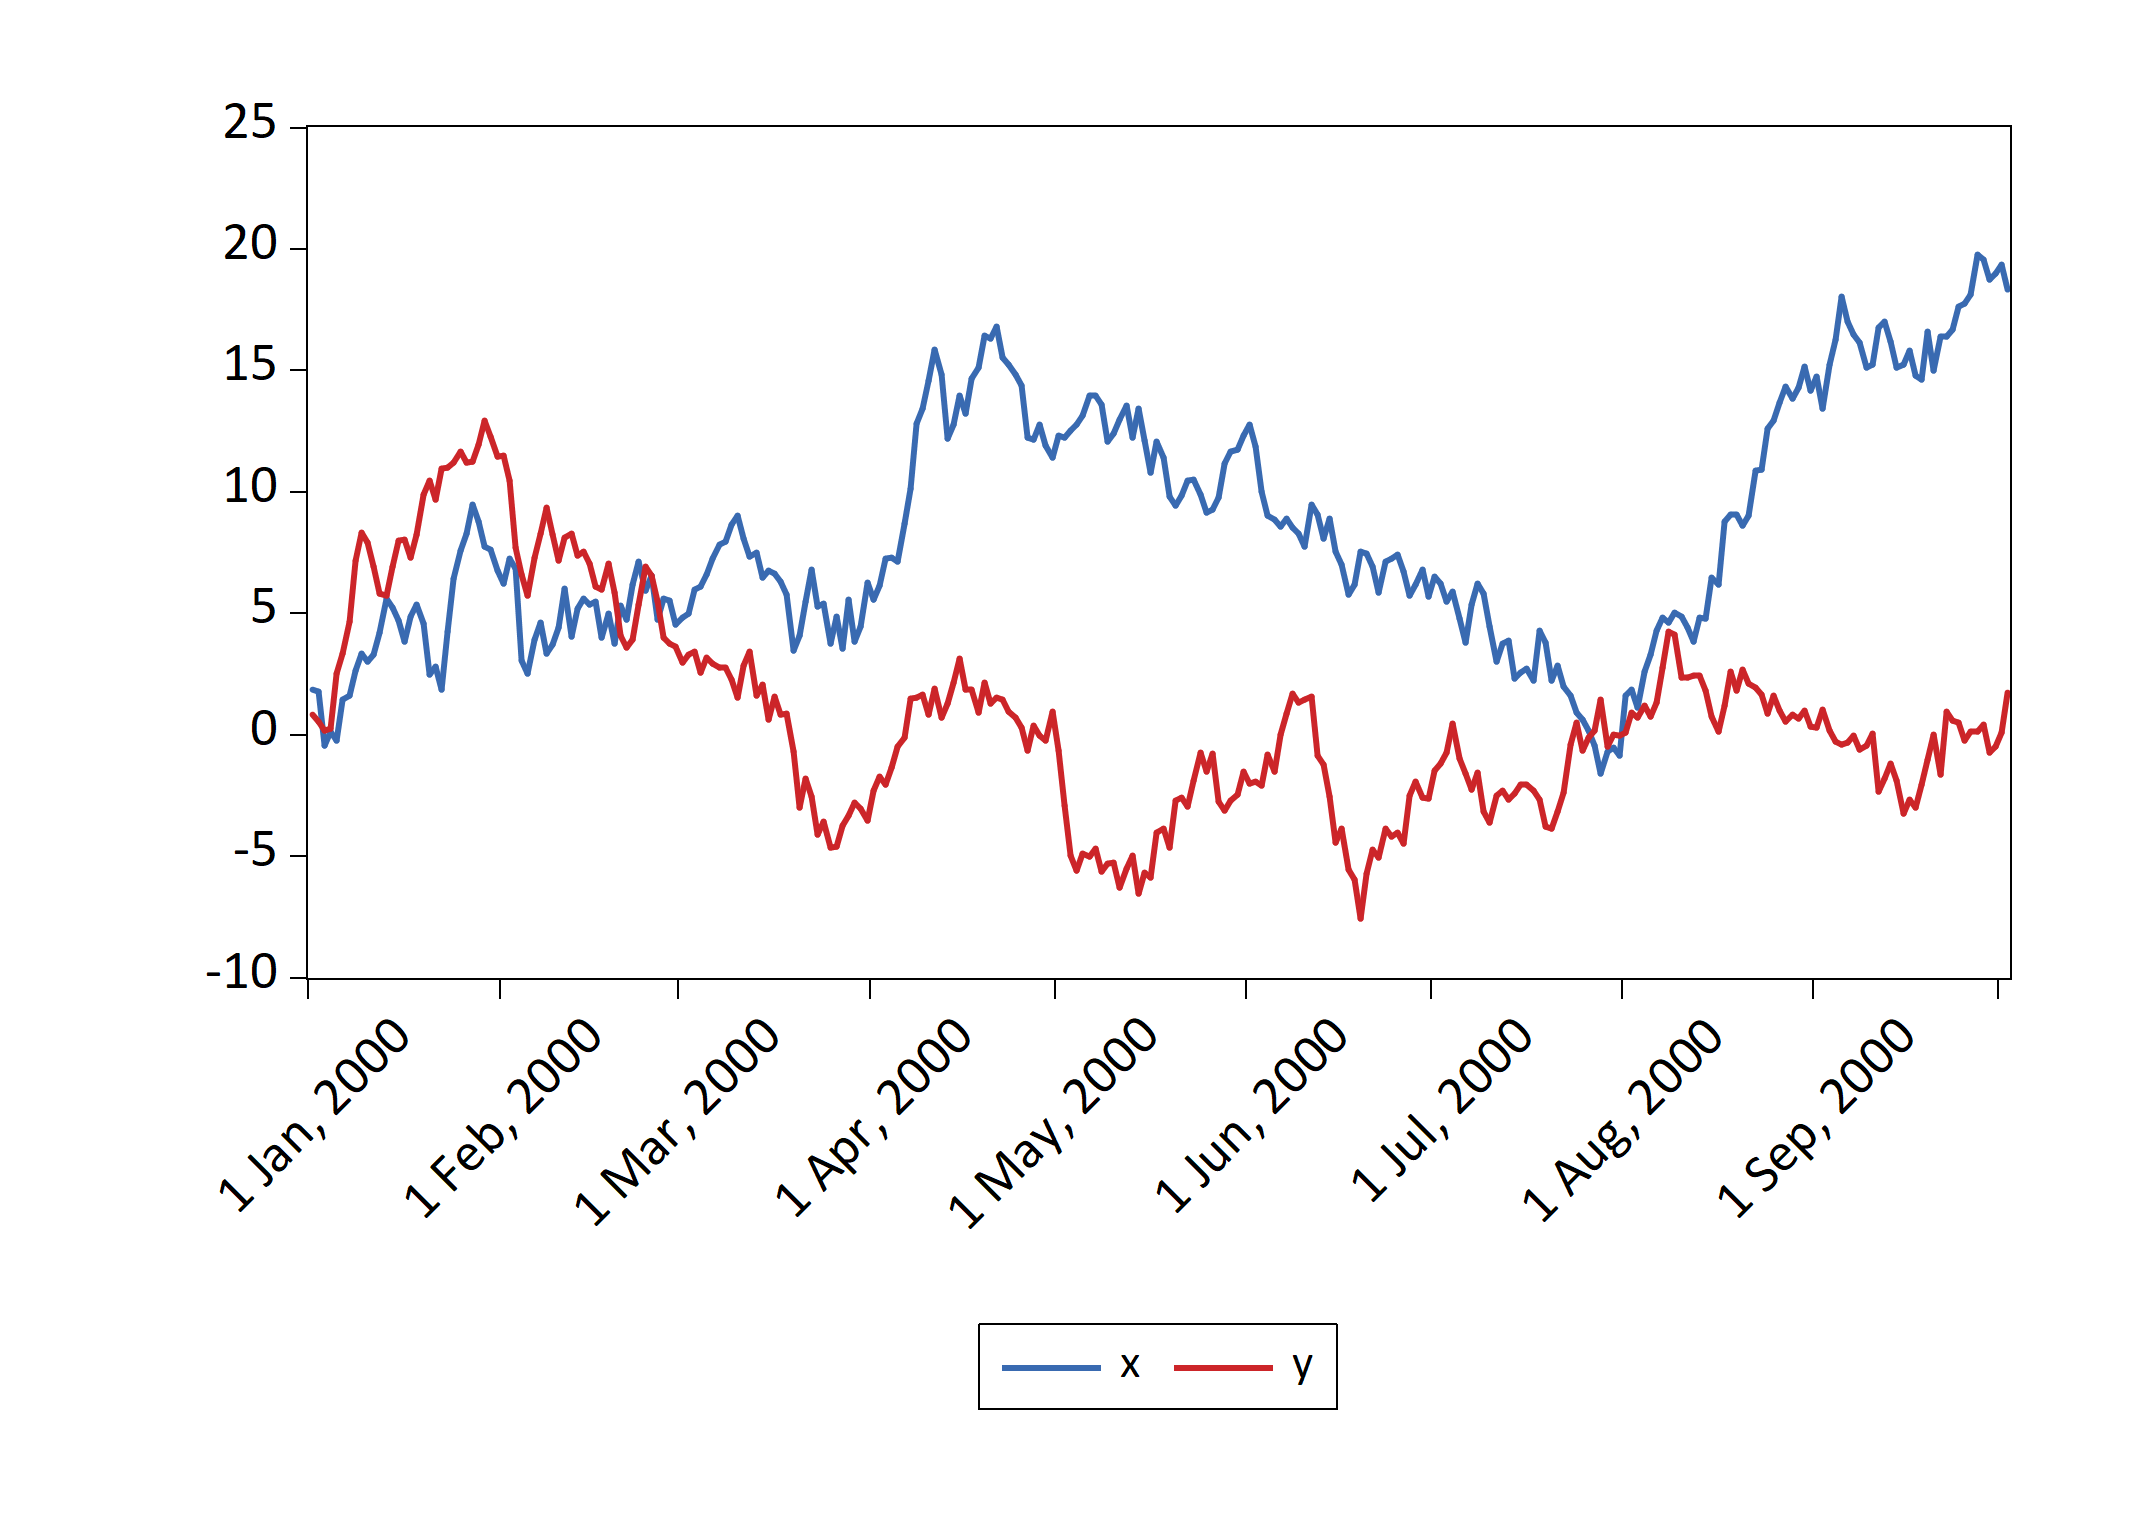
\includegraphics[width=0.9\linewidth,height=0.4\textheight]{figures/eviewsgraph3-eviewsgraph3-xy} 

}

\caption{EViews graph from dataframe (chunk: fig-eviewsGraph3)}\label{fig:fig-eviewsGraph3}
\end{figure}

To import EViews line graph of stacked values of the series objects as in Figure \ref{fig:fig-eviewsGraph4}:

\begin{verbatim}
EViews> import csvFile.csv @freq a start_date=2010
EViews> group some_group x y
EViews> freeze(eviewsGraph4_xy,mode=overwrite) some_group.line(s)
                    insert default values
EViews> eviewsGraph4_xy.save(t=png,d=300) eviewsGraph4_xy
\end{verbatim}

The R's syntax:

\begin{verbatim}
```{r} 
#| label: fig-eviewsGraph4
#| fig.cap: "EViews graph from dataframe (chunk: fig-eviewsGraph4)"
#| out.width: 90%
#| out.height: 40%
#| eval: TRUE
#| graph_procs: [template magazine, datelabel format("YYYY")]

eviews_graph(series=EviewsRDataFrame,frequency="m",start_date = "2010",
group = TRUE,graph_options="s")
```
\end{verbatim}

\begin{figure}

{\centering 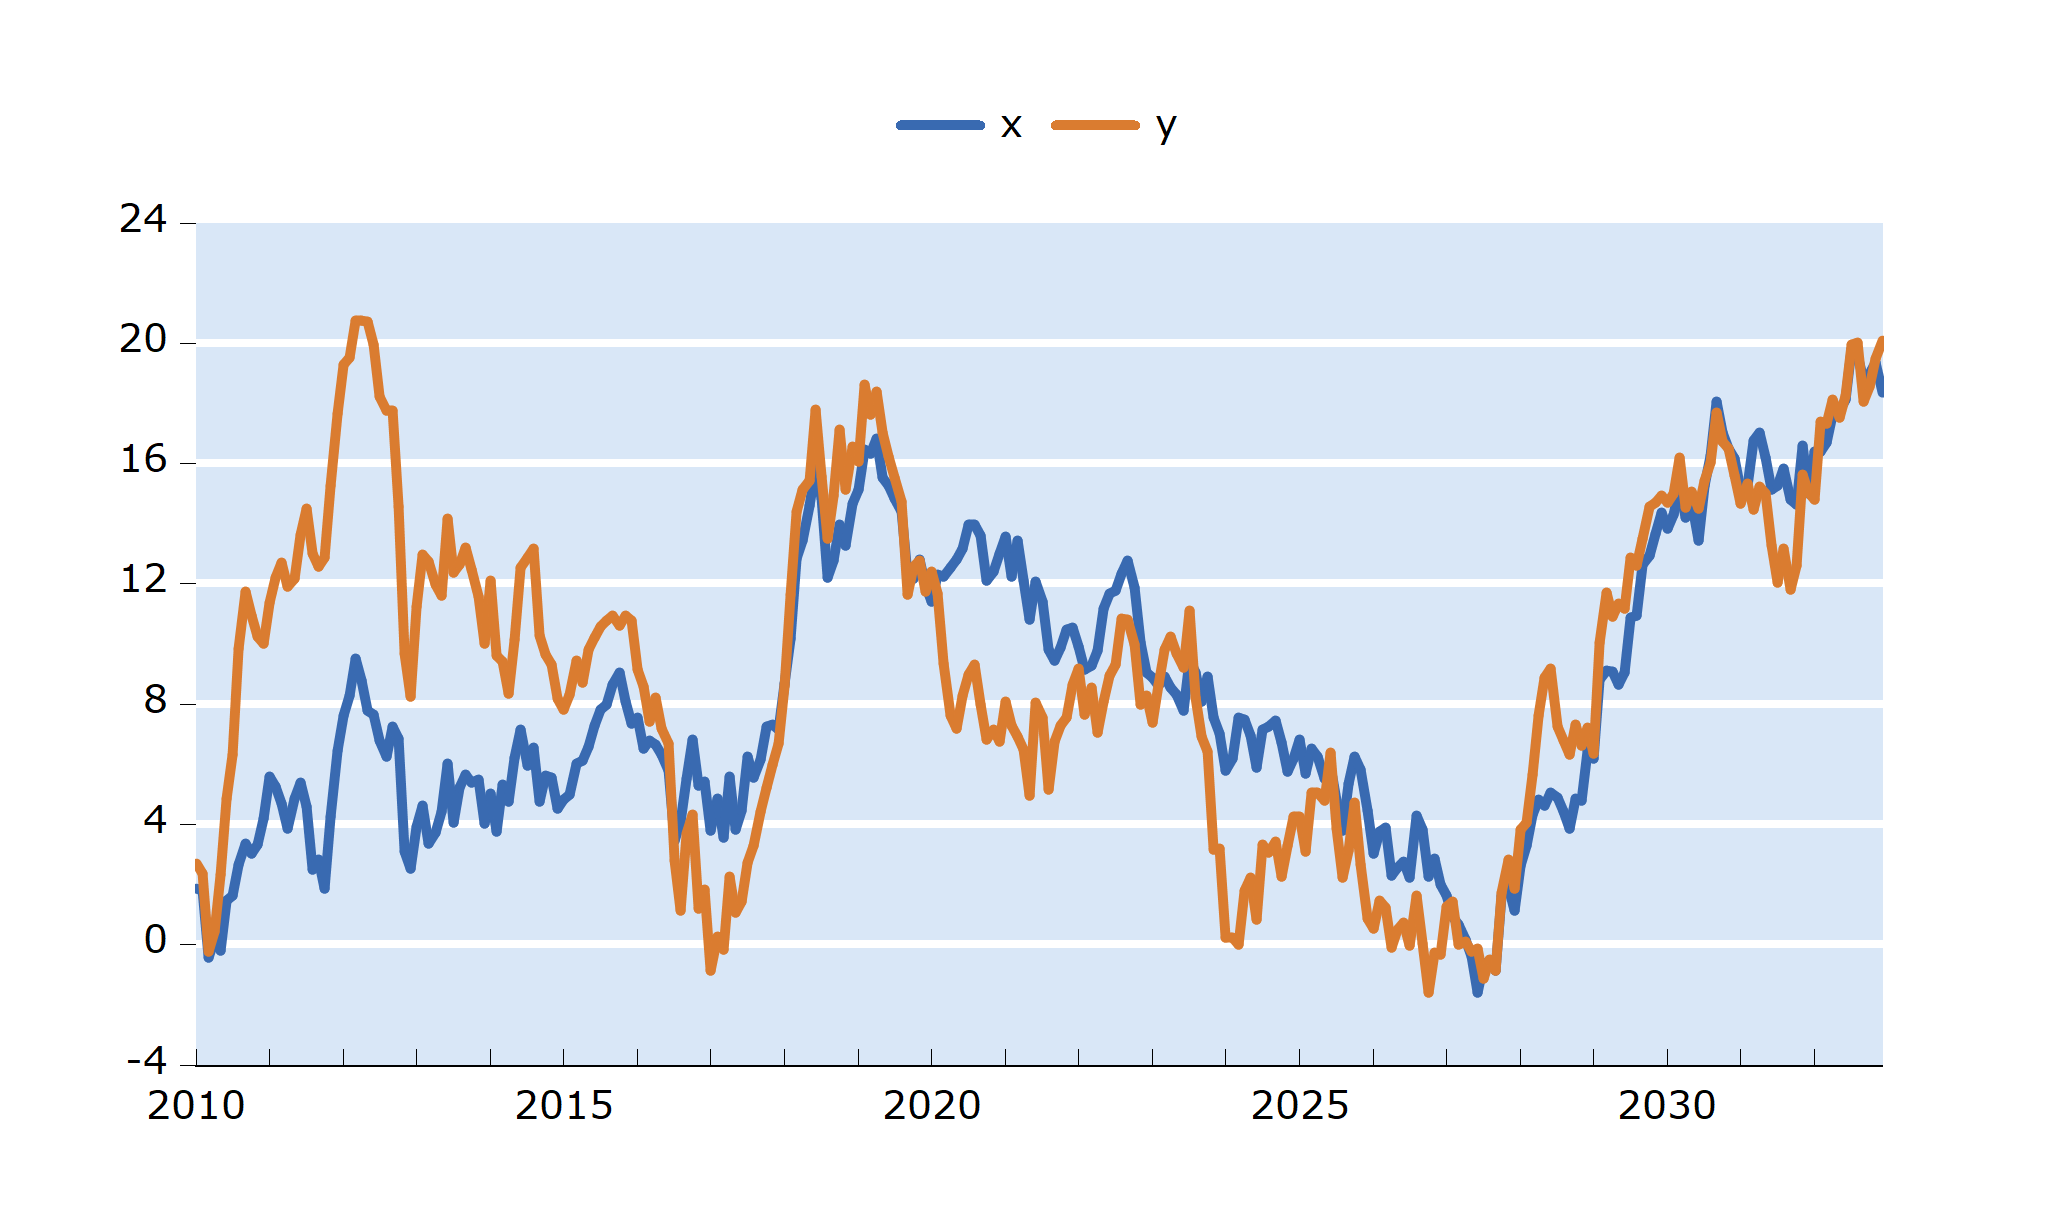
\includegraphics[width=0.9\linewidth,height=0.4\textheight]{figures/eviewsgraph4-eviewsgraph4-xy} 

}

\caption{EViews graph from dataframe (chunk: fig-eviewsGraph4)}\label{fig:fig-eviewsGraph4}
\end{figure}

Some journals require contributors to submit figures in black-and-white (see for example \protect\hyperlink{ref-Mati2023}{Mati, Civcir, and Ozdeser 2023}; \protect\hyperlink{ref-Mati2019c}{Mati, Civcir, and Ozdeser 2019}). Setting \texttt{graph\_procs=\textquotesingle{}template\ monochrome\textquotesingle{}} or \texttt{save\_options="t=png,-c"} gives the greyscale image as in Figure \ref{fig:fig-eviewsGraph5}. The difference is that the former overwrites all the graph modifications to match the monochrome template, while the latter only saves the graphs without any modifications.

\begin{figure}

{\centering 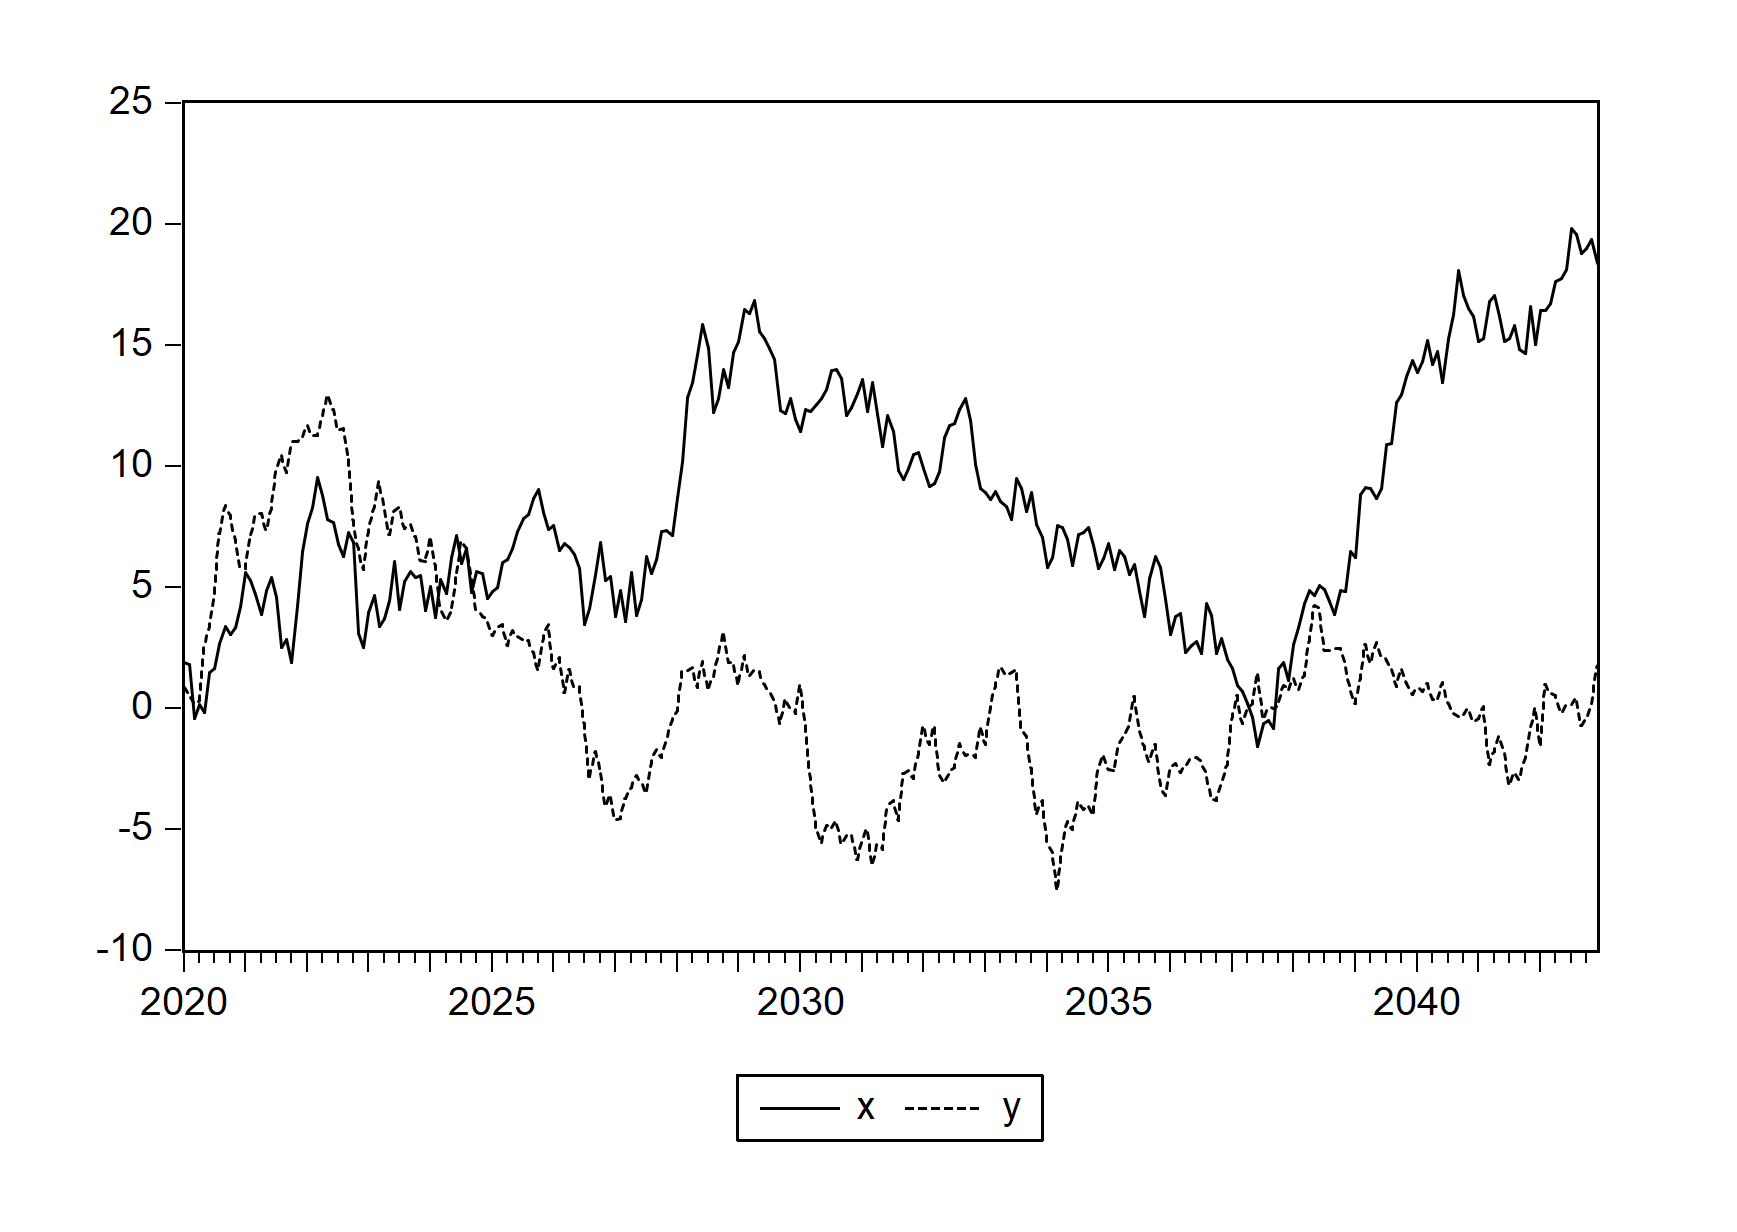
\includegraphics[width=0.9\linewidth,height=0.4\textheight]{figures/eviewsgraph5-eviewsgraph5-xy} 

}

\caption{EViews greyscale figure (chunk: fig-eviewsGraph5)}\label{fig:fig-eviewsGraph5}
\end{figure}

\hypertarget{the-eviews_import-function}{%
\subsection{The eviews\_import() function}\label{the-eviews_import-function}}

Data can be imported from external sources by \texttt{eviews\_import()} function. This function is a wrapper for EViews's \texttt{import} command. The EViews syntax is:

\begin{verbatim}
EViews> import([type=], options) source_description import_specification [@smpl smpl_string] 
+   [@genr genr_string] [@rename rename_string]
\end{verbatim}

To create a new workfile \texttt{eviews\_import.wf1} from \texttt{eviews\_import.csv}, which contains columns of x and y variables, using monthly series starting from 1990:

\begin{verbatim}
EViews> import EviewsR_files/eviews_import.csv @freq m 1990
EViews> wfsave EviewsR_files/eviews_import
\end{verbatim}

The R's syntax:

\begin{verbatim}
R> eviews_import(source_description = "EviewsR_Files/eviews_import.csv",
+     frequency = "m", start_date = "1990")
\end{verbatim}

To import \texttt{x} and \texttt{y}, with the former renamed to \texttt{x2}, from \texttt{eviews\_import.csv} into existing workfile \texttt{eviews\_import.wf1} within the sample of 1990m10 to 1992m11

\begin{verbatim}
EViews> wfopen EviewsR_files/eviews_import.wf1
EViews> import EviewsR_files/eviews_import.csv @smpl 1990m10 1992m11 @rename x x2
EViews> wfsave EviewsR_files/eviews_import
\end{verbatim}

\begin{verbatim}
R> eviews_import(source_description = "EviewsR_files/eviews_import.csv",
+     wf = "EviewsR_files/eviews_import", smpl_string = "1990m10 1992m11",
+     rename_string = "x x2")
\end{verbatim}

To import an R dataframe \texttt{EviewsRDataFrame} into \texttt{eviews\_import.wf1} workfile and simultaneously generate another series object \texttt{z} as the sum of \texttt{x} and \texttt{y}:

The dataframe needs to be written as \texttt{eviews\_import.csv} file using \texttt{write.csv()} function before executing the following code.

\begin{verbatim}
EViews> wfopen EviewsR_files/eviews_import.wf1
EViews> import EviewsR_files/eviews_import.csv @smpl 1990m10 1992m11 @genr z=x+y
EViews> wfsave EviewsR_files/eviews_import
\end{verbatim}

The R's syntax below makes the process easier:

\begin{verbatim}
R> eviews_import(source_description = EviewsRDataFrame, wf = "EviewsR_files/eviews_import",
+     genr_string = "z =x+y")
\end{verbatim}

To create a new workfile \texttt{eviews\_import1.wf1} from an R dataframe \texttt{EviewsRDataFrame} with a quarterly series starting from September, 2000:

\begin{verbatim}
R> eviews_import(source_description = EviewsRDataFrame, wf = "EviewsR_Files/eviews_import1",
+     frequency = "m", start_date = "2000m9")
\end{verbatim}

It is easier to plot a line graph of an undated dataframe with EviewsR than with the base R. For example, \texttt{eviews\_graph(dataFrame,start\_date=1990)} will graph a line plot labelled with dates starting from January 1990 on the x-axis. In base R, this requires creating a column for date in the dataframe or converting the dataframe to a timeseries object before plotting.\color{black}

\hypertarget{the-eviews_pagesave-function}{%
\subsection{The eviews\_pagesave() function}\label{the-eviews_pagesave-function}}

An EViews page can be saved in various formats by \texttt{eviews\_pagesave()} function.

\begin{verbatim}
EViews> pagesave(options) source_description table_description [@keep keep_list] [@drop drop_list]
+ [@keepmap keepmap_list] [@dropmap dropmap_list] [@smpl smpl_spec]
\end{verbatim}

To save \texttt{EviewsR} page from \texttt{EviewsR.wf1} workfile as a workfile named \texttt{eviews\_pagesave.wf1}:

\begin{verbatim}
EViews> wfopen EviewsR_files/EviewsR
EViews> pageselect eviewsr
EViews> pagesave eviews_pagesave
\end{verbatim}

The R's syntax:

\begin{verbatim}
R> eviews_pagesave(wf = "EviewsR_files/EviewsR", page = "EviewsR",
+     source_description = "EviewsR_files/eviews_pagesave")
\end{verbatim}

To save the first ten observations of series x only from \texttt{EviewsR} page of \texttt{EviewsR.wf1} workfile in a \texttt{CSV} file named \texttt{eviews\_pagesave.csv}:

\begin{verbatim}
EViews> wfopen EviewsR_files/EviewsR
EViews> pageselect eviewsr
EViews> pagesave eviews_pagesave.csv @keep x @smpl @first @first+9
\end{verbatim}

\begin{verbatim}
R> eviews_pagesave(wf = "EviewsR_files/EviewsR", page = "EviewsR",
+     source_description = "EviewsR_files/eviews_pagesave.csv",
+     keep_list = "x", smpl_spec = "@first @first+9")
\end{verbatim}

Similarly, the values of \texttt{keepmap\_list} and \texttt{dropmap\_list} can be set as \texttt{keepmap\_list="y*"} and \texttt{dropmap\_list="x?"} respectively.

\hypertarget{the-eviews_wfcreate-function}{%
\subsection{The eviews\_wfcreate() function}\label{the-eviews_wfcreate-function}}

An EViews workfile can be created using \texttt{eviews\_wfcreate()} function in R.

\begin{verbatim}
EViews> wfcreate(options) frequency[(subperiod_opts)] start_date end_date [num_cross_sections]

EViews> wfcreate(options) frequency[(subperiod_opts)] start_date +num_observations

EViews> wfcreate(options) u num_observations
\end{verbatim}

To create an EViews workfile \texttt{eviews\_wfcreate.wf1} along with a page named \texttt{EviewsR\_page} in \texttt{EviewsR\_files/} folder:

\begin{verbatim}
EViews> cd EviewsR_files
EViews> wfcreate(wf=eviews_wfcreate,page=EviewsR_page) m 2000 2022
EViews> wfsave eviews_wfcreate
\end{verbatim}

The R's syntax:

\begin{verbatim}
R> eviews_wfcreate(wf = "eviews_wfcreate", page = "EviewsR_page",
+     frequency = "m", start_date = "2000", end_date = "2022",
+     save_path = "EviewsR_files")
\end{verbatim}

\hypertarget{the-eviews_wfsave-function}{%
\subsection{The eviews\_wfsave() function}\label{the-eviews_wfsave-function}}

An EViews workfile can be saved in various output formats using \texttt{eviews\_wfsave()} function in R.

\begin{verbatim}
EViews> wfsave(options) [path\]filename

EViews> wfsave(options) source_description [@keep keep_list] [@drop drop_list]
+ [@keepmap keepmap_list] [@dropmap dropmap_list] [@smpl smpl_spec]

EViews> wfsave(options) source_description table_description [@keep keep_list]
+ [@drop drop_list] [@keepmap keepmap_list] [@dropmap dropmap_list] [@smpl smpl_spec]
\end{verbatim}

To save all series objects in \texttt{EviewsR} page of \texttt{EviewsR.wf1} workfile except x in \texttt{eviews\_wfsave.csv} file:

\begin{verbatim}
EViews> wfopen EviewsR_files/eviewsr
EViews> pageselect eviewsr
EViews> wfsave eviews_wfsave.csv @drop x 
\end{verbatim}

\begin{verbatim}
R> eviews_wfsave(wf = "EviewsR_files/EviewsR", page = "eviewsr",
+     source_description = "EviewsR_files/eviews_wfsave.csv", drop_list = "x")
\end{verbatim}

\hypertarget{the-exec_commands-function}{%
\subsection{The exec\_commands() function}\label{the-exec_commands-function}}

A set of EViews commands can be executed with the help of \texttt{exec\_commands()} function in R.

The EViews chunk in Section \ref{sec-document} can be translated using this function as follows:

\begin{verbatim}
R> exec_commands(c("'This is some comment in EViews program, feel free to write anything",
+   
+   'wfcreate(wf=EviewsR,page=EviewsR) m 2000 2022',
+ 
+   'for %y EviewsR1 EviewsR2',
+   'pagecreate(page={%y}) m 2000 2022',
+   'next',
+ 
+   'for %y EviewsR EviewsR1 EviewsR2',
+   
+   'pageselect {%y}',
+   
+   'genr y=@cumsum(nrnd)',
+   'genr x=@cumsum(nrnd)',
+   
+   'graph x_graph.line(o=eviews5) x',
+   'graph y_graph.dot(o=bokeh) y',
+   
+   'table EviewsRTable',
+ 
+   'for !j=1 to 7',
+   'EviewsRTable(1,{!j})="Header"+" "+@str({!j})',
+   'next',
+ 
+   'for !i=1 to 10',
+   'for !j=1 to 7',
+   'EviewsRTable({!i}+1,{!j})=@str({!i})+","+@str({!j})',
+   'next',
+   'next ',
+ 
+   'next',
+   
+   'wfsave EviewsR_files/EviewsR'))
\end{verbatim}

Alternatively, we can assign the EViews commands to an object before calling the function:

\begin{verbatim}
R> commands=r'('This is some comment in EViews program, feel free to write anything
+   
+   wfcreate(wf=EviewsR,page=EviewsR) m 2000 2022
+ 
+   for %y EviewsR1 EviewsR2
+   pagecreate(page={%y}) m 2000 2022
+   next
+ 
+   for %y EviewsR EviewsR1 EviewsR2
+   
+   pageselect {%y}
+   
+   genr y=@cumsum(nrnd)
+   genr x=@cumsum(nrnd)
+   
+   graph x_graph.line(o=eviews5) x
+   graph y_graph.dot(o=bokeh) y
+   
+   table EviewsRTable
+ 
+   for !j=1 to 7
+   EviewsRTable(1,{!j})="Header"+" "+@str({!j})
+   next
+ 
+   for !i=1 to 10
+   for !j=1 to 7
+   EviewsRTable({!i}+1,{!j})=@str({!i})+","+@str({!j})
+   next
+   next 
+ 
+   next
+   
+   wfsave EviewsR_files/EviewsR)'
R> exec_commands(commands)
\end{verbatim}

To create a workfile \texttt{exec\_commands1.wf1} using a monthly frequency from November, 2000 to January 2022:

\begin{verbatim}
EViews> cd EviewsR_files
EViews> wfcreate(wf=exec_commands1,page=Page) m 2000m11 2022m1
EViews> %wf=@wfname
EViews> wfsave {%wf}
EViews> exit
\end{verbatim}

The base R's syntax:

\begin{verbatim}
R> exec_commands(c("cd EviewsR_files", "wfcreate(wf=exec_commands1,page=Page) m 2000m11 2022m1"))
\end{verbatim}

To execute EViews commands on an existing EViews workfile like the one created above:

\begin{verbatim}
EViews> wfopen EviewsR_files/exec_commands1
EViews> pageselect EviewsR
EViews> genr x=@cumsum(nrnd)
EViews> genr y=@cumsum(nrnd)
EViews> genr z=x+y
EViews> delete(noerr) grap
EViews> graph grap.line x y z
EViews> %wf=@wfname
EViews> wfsave {%wf}
EViews> exit
\end{verbatim}

The R's syntax:

\begin{verbatim}
R> exec_commands(commands = c("genr x=@cumsum(nrnd)", "genr y=@cumsum(nrnd)",
+     "genr z=x+y", "delete(noerr) grap", "graph grap.line x y z"),
+     wf = "EviewsR_files/exec_commands1", page = "page")
\end{verbatim}

\hypertarget{the-export_dataframe-function}{%
\subsection{The export\_dataframe() function}\label{the-export_dataframe-function}}

Use \texttt{export\_dataframe()} function to export dataframe object to EViews as a workfile.

To export the dataframe \texttt{EviewsRDataFrame} as a workfile \texttt{export\_dataframe.wf1} with monthly frequency starting from January 1990:

\begin{verbatim}
R> export_dataframe(source_description = EviewsRDataFrame, wf = "EviewsR_files/export_dataframe",
+     start_date = "1990", frequency = "m")
\end{verbatim}

To export the dataframe as a workfile \texttt{export\_dataframe1.wf1} with undated frequency. However, if the dataframe contains a column with a regular dated frequency, EViews will automatically detect the date series and create a dated workfile.

\begin{verbatim}
R> export_dataframe(source_description = EviewsRDataFrame, wf = "EviewsR_files/export_dataframe1")
\end{verbatim}

\hypertarget{the-import_equation-function}{%
\subsection{The import\_equation() function}\label{the-import_equation-function}}

The data members of the EViews equation objects are imported in R as a dataframe.

The data members are accessible via:

\begin{itemize}
\item
  \texttt{eviews\$pageName\_equationName\$dataMember} in base R or
\item
  \texttt{chunkLabel\$pageName\_equationName\$dataMember} in an R Markdown or Quarto document.
\end{itemize}

To get the value of Akaike Information Criterion (AIC) of an equation object named \texttt{OLS} on page \texttt{EviewsR} into base R:

\begin{verbatim}
R> eviews$eviewsr_ols$aic
\end{verbatim}

To obtain the same value from the same equation object in an R Markdown or Quarto document, if the \texttt{import\_equation()} function is called from a chunk label \texttt{importEquation}:

\begin{verbatim}
R> importEquation$eviewsr_ols$aic
\end{verbatim}

Note that the \texttt{equation}, \texttt{graph}, \texttt{series} and \texttt{table} objects do not need the chunk label in base R. However, where an R environment is required, we use \texttt{eviews} instead of the chunk label.

\hypertarget{the-import_graph-function}{%
\subsection{The import\_graph() function}\label{the-import_graph-function}}

Importing existing graph objects from EViews workfile is easy with \texttt{import\_graph()} function.

The R chunk below imports EViews graph objects \texttt{x\_graph} and \texttt{y\_graph} into an R Markdown or Quarto document as Figure \ref{fig:fig-importGraph}. Use \texttt{graph="*"} and \texttt{page="*"} to import all EViews graph objects across all the workfile pages. The \texttt{graph} argument accepts any valid EViews pattern or wildcard expressions, such as \texttt{graph="x\_*"}, \texttt{graph="?\_graph"}\}. Both the \texttt{graph} and \texttt{page} arguments can be used to choose specific graph object(s) and workfile page(s) respectively.

To import all graph objects from \texttt{EviewsR2} of \texttt{EviewsR.wf1} workfile that lives in \texttt{EviewsR\_files/} folder:

\begin{verbatim}
```{r} 
#| label: fig-importGraph
#| fig.cap: "Existing EViews graph imported (chunk: fig-importGraph)"
#| out.width: 45%
#| out.height: 15%

import_graph(wf="EviewsR_files/EviewsR",page="eviewsr2")
```
\end{verbatim}

\begin{figure}

{\centering 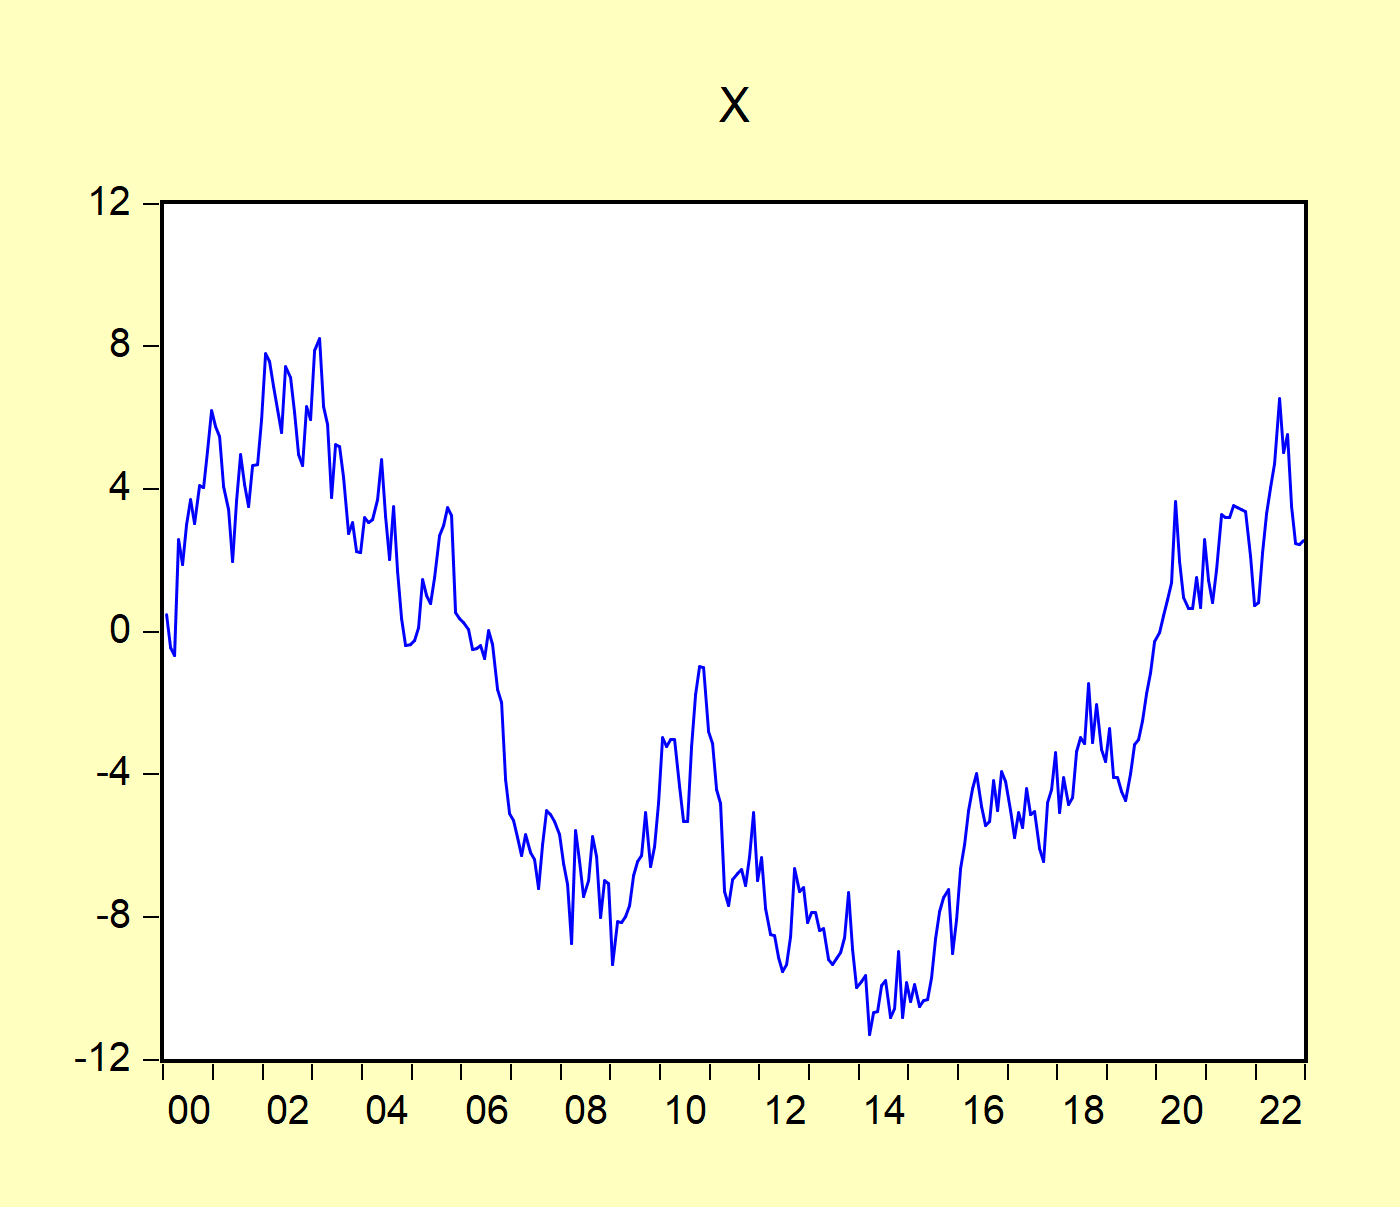
\includegraphics[width=0.45\linewidth,height=0.15\textheight]{figures/fig-importgraph-eviewsr2-x_graph} 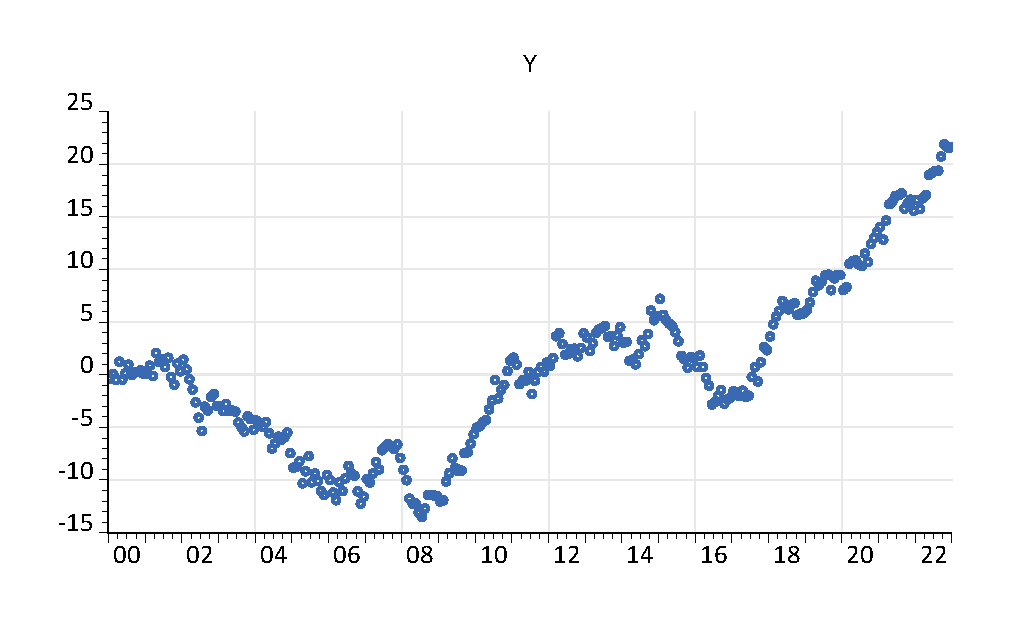
\includegraphics[width=0.45\linewidth,height=0.15\textheight]{figures/fig-importgraph-eviewsr2-y_graph} 

}

\caption{Existing EViews graph imported (chunk: fig-importGraph)}\label{fig:fig-importGraph}
\end{figure}

\hypertarget{sec-importtable}{%
\subsection{The import\_kable() function}\label{sec-importtable}}

EViews table objects can be imported as \texttt{kable} object by \texttt{import\_kable()} function.

To import the entire table object \texttt{EviewsRTable} from \texttt{EviewsR} page of \texttt{EviewsR.wf1} workfile as Table \ref{tab:tbl-importKable}:

\begin{verbatim}
R> import_kable(wf = "EviewsR_files/EviewsR", page = "EviewsR",
+     table = "EviewsRTable", caption = "EViews table imported as kable",
+     format = ifelse(is_html_output(), "html", "latex"), linesep = "")
\end{verbatim}

\begin{table}

\caption{\label{tab:tbl-importKable}EViews table imported as kable}
\centering
\begin{tabular}[t]{l|l|l|l|l|l|l}
\hline
Header 1 & Header 2 & Header 3 & Header 4 & Header 5 & Header 6 & Header 7\\
\hline
1,1 & 1,2 & 1,3 & 1,4 & 1,5 & 1,6 & 1,7\\
2,1 & 2,2 & 2,3 & 2,4 & 2,5 & 2,6 & 2,7\\
3,1 & 3,2 & 3,3 & 3,4 & 3,5 & 3,6 & 3,7\\
4,1 & 4,2 & 4,3 & 4,4 & 4,5 & 4,6 & 4,7\\
5,1 & 5,2 & 5,3 & 5,4 & 5,5 & 5,6 & 5,7\\
6,1 & 6,2 & 6,3 & 6,4 & 6,5 & 6,6 & 6,7\\
7,1 & 7,2 & 7,3 & 7,4 & 7,5 & 7,6 & 7,7\\
8,1 & 8,2 & 8,3 & 8,4 & 8,5 & 8,6 & 8,7\\
9,1 & 9,2 & 9,3 & 9,4 & 9,5 & 9,6 & 9,7\\
10,1 & 10,2 & 10,3 & 10,4 & 10,5 & 10,6 & 10,7\\
\hline
\end{tabular}
\end{table}

To import certain range of the table object \texttt{EviewsRTable} as Table \ref{tab:tbl-importKable1}:

\begin{verbatim}
R> import_kable(wf = "EviewsR_files/EviewsR", page = "EviewsR",
+     table = "EviewsRTable", range = "r1c2:r5c6", digits = 3,
+     caption = "Selected cells of EViews table imported as kable",
+     format = ifelse(is_html_output(), "html", "latex"))
\end{verbatim}

\begin{table}

\caption{\label{tab:tbl-importKable1}Selected cells of EViews table imported as kable}
\centering
\begin{tabular}[t]{l|l|l|l|l}
\hline
Header 2 & Header 3 & Header 4 & Header 5 & Header 6\\
\hline
1,2 & 1,3 & 1,4 & 1,5 & 1,6\\
\hline
2,2 & 2,3 & 2,4 & 2,5 & 2,6\\
\hline
3,2 & 3,3 & 3,4 & 3,5 & 3,6\\
\hline
4,2 & 4,3 & 4,4 & 4,5 & 4,6\\
\hline
5,2 & 5,3 & 5,4 & 5,5 & 5,6\\
\hline
\end{tabular}
\end{table}

\hypertarget{the-import_series-function}{%
\subsection{The import\_series() function}\label{the-import_series-function}}

Use \texttt{import\_series()} function to import EViews series objects into R as a dataframe or \texttt{xts} object. The function creates a new environment \texttt{eviews}, whose objects can be accessed via \texttt{eviews\$pageName} in base R or \texttt{chunkLabel\$pageName} in R Markdown or Quarto.

To import EViews series objects from \texttt{EviewsR} page of \texttt{EviewsR.wf1} workfile into R as a dataframe:

\begin{verbatim}
R> import_series(wf = "EviewsR_files/EviewsR", page = "EviewsR")
\end{verbatim}

To access the imported series of \texttt{EviewsR} page in base R:

\begin{verbatim}
R> eviews$eviewsr
\end{verbatim}

To access the imported series of \texttt{EviewsR} page in an R Markdown or Quarto document, if the chunk label is \texttt{importSeries}:

\begin{verbatim}
R> importSeries$eviewsr
\end{verbatim}

The \texttt{series} argument can take any valid EViews wildcard expressions. The series objects are imported to EViews as a dataframe with date column as \texttt{POSIXct} by default. We can import the series as \texttt{xts} object by setting \texttt{class="xts"}.

\begin{verbatim}
R> import_series(wf = "EviewsR_files/EviewsR", page = "EviewsR",
+     class = "xts")
\end{verbatim}

\hypertarget{the-import_table-function}{%
\subsection{The import\_table() function}\label{the-import_table-function}}

Use \texttt{import\_table()} function to import EViews table objects into R as a dataframe. The imported table objects can be accessed via \texttt{eviews\$pageName\_tableName}.

\begin{verbatim}
R> import_table(wf = "", page = "*", table = "*")
\end{verbatim}

The \texttt{table} argument accepts valid EViews wildcard expressions.

To import all the table objects in \texttt{EviewsR.wf1}:

\begin{verbatim}
R> import_table(wf = "EviewsR_files/EviewsR")
\end{verbatim}

To import \texttt{eviewsrtable} from the same workfile but from a page named \texttt{EviewsR} only:

\begin{verbatim}
R> import_table(wf = "EviewsR_files/EviewsR", page = "EviewsR",
+     table = "eviewsrtable")
\end{verbatim}

To get the table imported from \texttt{EviewsR} in an R Markdown or Quarto document, if the chunk label is \texttt{importTable1}:

\begin{verbatim}
R> importTable1$eviewsr_eviewsrtable
\end{verbatim}

\hypertarget{the-import_workfile-function}{%
\subsection{The import\_workfile() function}\label{the-import_workfile-function}}

To import EViews equation, graph, series and table objects at once from an existing workfile, use the \texttt{import\_workfile()} function. This function is a combination of \texttt{import\_equation()}, \texttt{import\_graph()}, \texttt{import\_series()} and \texttt{import\_table()} functions.

To import all the EViews equation, graph, series and table objects from the \texttt{EviewsR.wf1} workfile.

\begin{verbatim}
```{r} 
#| label: fig-importWorkfile
#| fig.cap: Graphs imported by EViews chunk (fig-importWorkfile)
#| out.width: 45%
#| out.height: 15%

import_workfile("EviewsR_files/EviewsR")
```
\end{verbatim}

We can also obtain the imported EViews equation, series and table objects in the same way as \texttt{import\_equation()}, \texttt{import\_series()} and \texttt{import\_table()}.

\hypertarget{the-rwalk-function}{%
\subsection{The rwalk() function}\label{the-rwalk-function}}

A set of random walk series can be simulated in R using EViews engine, thanks to \texttt{rwalk()} function. The random walk series objects are returned as R dataframe, which can be accessed as \texttt{eviews\$seriesNames} in base R and as \texttt{chunkLabel\$seriesNames} in an R Markdown or Quarto document. Removing space from the value(s) of the \texttt{series} argument provides the \texttt{seriesNames}. Setting argument \texttt{class="xts"} returns \texttt{xts} object instead of dataframe. This function can be used to replicate examples provided in Econometrics textbooks that use EViews, as random numbers generated in R and EViews differ.

To generate random walk series X Y and Z using EViews and imports them into R as a dataframe \texttt{eviews\$XYZ\}}:

\begin{verbatim}
R> rwalk(series = "X Y Z", rndseed = 12345, start_date = "1990",
+     frequency = "M", num_observations = 276)
\end{verbatim}

To generate random series rw1, rw2 and rw3 each with a drift of 10, on the existing workfile \texttt{EviewsR.wf1}:

\begin{verbatim}
R> rwalk(wf = "EviewsR_files/EviewsR", series = "rw1 rw2 rw3", rndseed = 12345,
+     drift = 10)
\end{verbatim}

To obtain the head in base R:

\begin{verbatim}
R> head(eviews$rw1rw2rw3)
\end{verbatim}

To get the head in an R Markdown or Quarto document, if the chunk label is \texttt{rwalk1}:

\begin{verbatim}
R> head(rwalk1$rw1rw2rw3)
\end{verbatim}

To plot the random walk dataframe with both \CRANpkg{ggplot2} package (\protect\hyperlink{ref-Wickham2016}{Wickham 2016}) and \texttt{eviews\_graph()} function as shown in Figure \ref{fig:fig-rwalk}:

\begin{verbatim}
```{r}  
#| label: fig-rwalk
#| out.width: 45%
#| out.height: 15%
#| dim: [7,4]
#| fig.cap: "Random walk generated by EViews"
#| fig.subcap: ["Graph from ggplot package","Graph from EviewsR package"]

ggplot(rwalk$XYZ,aes(x=date)) +
    geom_line(aes(y=x,color="x"))+ geom_line(aes(y=y,color="y"))+
    geom_line(aes(y=z,color="z"))+
  xlab('')+ylab('')+
  labs(colour = "")+
  scale_color_manual(values=c(x="blue",y="red",z="#008753"))
  
eviews_graph(series=rwalk$XYZ,group = TRUE,graph_procs=c('template reverse','legend position(right)'))

```
\end{verbatim}

\begin{figure}

{\centering \subfloat[Graph from ggplot2 package\label{fig:fig-rwalk-1}]{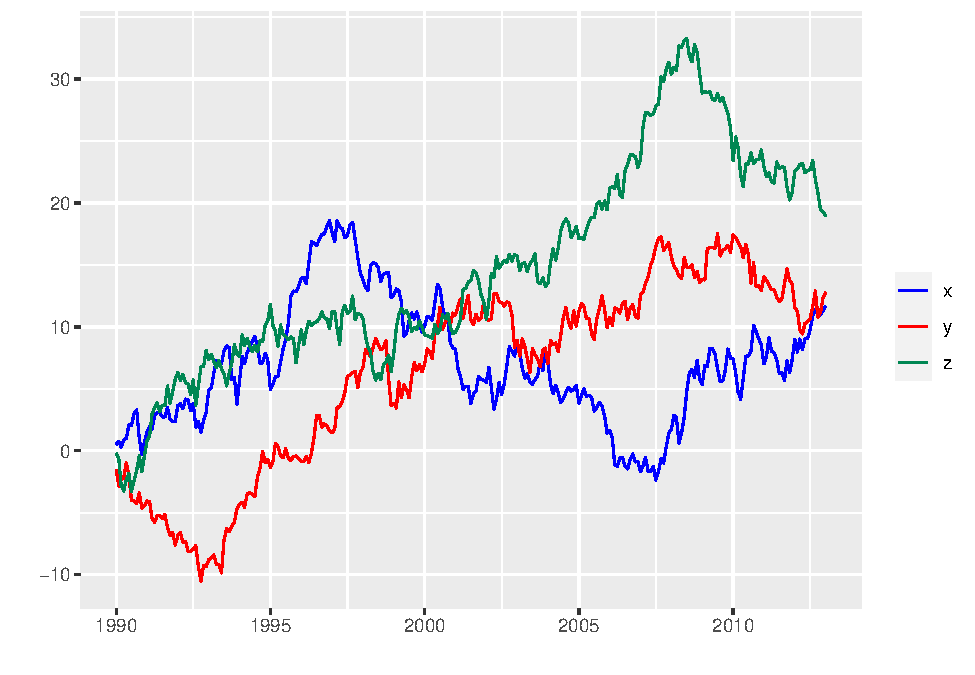
\includegraphics[width=0.45\linewidth,height=0.15\textheight]{figures/fig-rwalk-1} }\subfloat[Graph from EviewsR package\label{fig:fig-rwalk-2}]{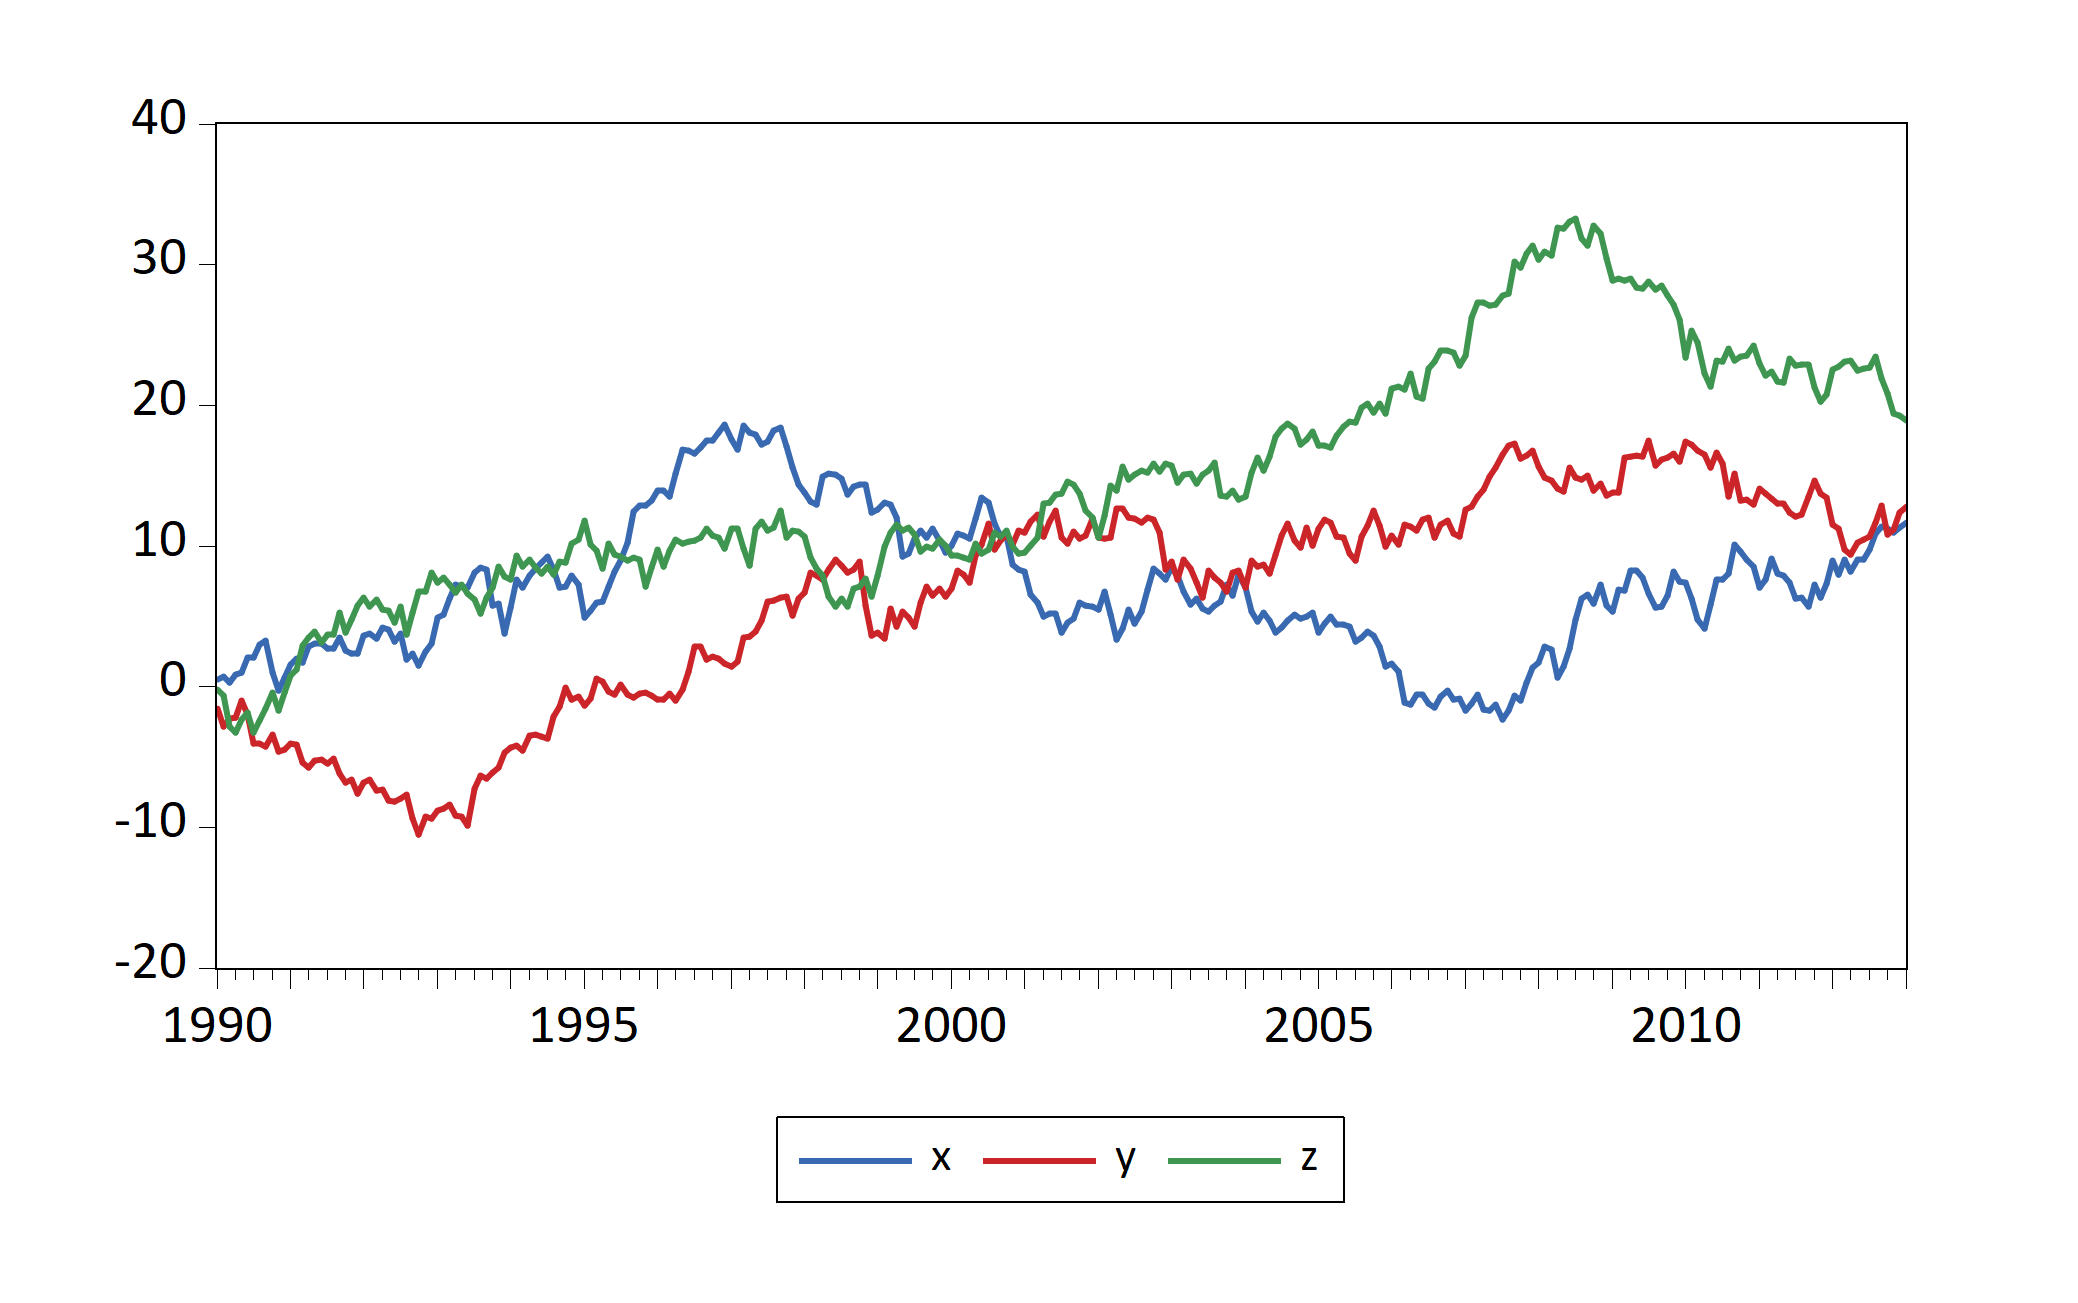
\includegraphics[width=0.45\linewidth,height=0.15\textheight]{figures/rwalk-rwalk-xyz} }

}

\caption{Random walk generated by EViews}\label{fig:fig-rwalk}
\end{figure}

\hypertarget{the-set_eviews_path-function}{%
\subsection{The Set\_eviews\_path() function}\label{the-set_eviews_path-function}}

In case of non-standard EViews installation or presence of more than one EViews executable and we do not want to use the latest, we can use this function to set the path to the EViews executable:

To use EViews executable \texttt{EViews10}:

\begin{verbatim}
R> set_eviews_path("C:/Program Files (x86)/EViews 10/EViews10.exe")
\end{verbatim}

or

\begin{verbatim}
R> set_eviews_path("EViews10")
\end{verbatim}

\hypertarget{sec-implementation}{%
\section{Package implementation}\label{sec-implementation}}

The purpose of this section to explain how the package is implemented, so that contributions for further development of the package can be easy and straightforward. We show how the \texttt{eviews} knit-engine is added and how the base R functions are created.

\hypertarget{sec-knit-engine}{%
\subsection{Adding eviews as knit-engine}\label{sec-knit-engine}}

As mentioned earlier, \CRANpkg{EviewsR} (\protect\hyperlink{ref-Mati2019}{Mati 2019b}) package adds a knit-engine for Econometric Views (EViews), which is a proprietary econometric software package. The behaviour of EViews is listed below:

\begin{enumerate}
\def\labelenumi{\arabic{enumi}.}
\item
  The file extension of \texttt{eviews} code file is \texttt{.prg}.
\item
  The command line execution of the \texttt{eviews} code file requires running \texttt{"eviewsExecutable\ exec\ EviewsFileName.prg"} or opening the \texttt{.prg} file.
\item
  The \texttt{eviews} code file can be opened by quoting the path to the EViews program file. If the EViews code file lives in the current working directory (CWD), writing its full file name (together with the \texttt{.prg} extension), with or without the quotes, will run the \texttt{eviews} code file.
\end{enumerate}

The first step is to create a character string with the EViews's \texttt{.prg} file extension. For example, a character string \texttt{"MyEviewsFile.prg"} can be assigned to an object \texttt{fileName} using the code \texttt{fileName\ \textless{}-"MyEviewsFile.prg"}. The second step is to create another R object (\texttt{eviewsCode}) and use \texttt{writeLines()} function to write the EViews code to the file name object created in step 1. The code \texttt{writeLines(eviewsCode,fileName)} creates a file in the EViews's CWD and names it \texttt{MyEviewsFile.prg}. The third step is to execute the file \texttt{MyEviewsFile.prg} using \texttt{system2()} function. The code \texttt{system2(\textquotesingle{}EViewsExecutable\textquotesingle{},\textquotesingle{}exec\ path/to/EViewsFileName.prg\textquotesingle{})} opens and executes the EViews code file \texttt{MyEviewsFile.prg}. The last step is to use \texttt{.onLoad()} function along with a function from \CRANpkg{knitr} package \texttt{knit\_engines\$set(eviews=eng\_eviews)} to set \texttt{eviews} as the knit-engine for EViews. Figure \ref{fig:EngineSteps} presents four easy steps for adding \texttt{eviews} to the existing \CRANpkg{knitr} engines and creating the R functions.

\hypertarget{creating-base-r-functions}{%
\subsection{Creating base R functions}\label{creating-base-r-functions}}

The base R functions are created in a way similar to adding the knit-engine, but they do not depend on \CRANpkg{knitr} package. For the sake of demonstration, we use \texttt{eviews\_wfsave()} function, which saves EViews workfile in various formats. The EViews syntax for \texttt{wfsave} command is as follows:

\begin{verbatim}
EViews> wfsave(options) [path\]filename

EViews> wfsave(options) source_description [@keep keep_list] [@drop drop_list] 
+ [@keepmap keepmap_list] [@dropmap dropmap_list] [@smpl smpl_spec]

EViews> wfsave(options) source_description table_description [@keep keep_list] 
+[@drop drop_list] [@keepmap keepmap_list] [@dropmap dropmap_list] [@smpl smpl_spec]
\end{verbatim}

The last line of the code provides a more general syntax than the first two. Therefore, we use it to create the equivalent base R function. The syntax contains optional arguments such as \texttt{@keep\ keep\_list}, \texttt{@drop\ drop\_list}, \texttt{@drop\ drop\_list}, \texttt{@dropmap\ dropmap\_list}, \texttt{@smpl\ smpl\_spec}, which are enclosed in square brackets. The arguments \texttt{options}, \texttt{source\_description} and \texttt{table\_description} are essential. In addition to this, we need to distinguish constant arguments from variable arguments. The constants include \texttt{wfsave}, \texttt{@keep}, \texttt{@drop}, \texttt{@keepmap} and \texttt{@dropmap}. On the other hand, the variables, which users can change, include \texttt{options}, \texttt{source\_description}, \texttt{table\_description}, \texttt{keep\_list}, \texttt{drop\_list}, \texttt{drop\_list}, \texttt{dropmap\_list}, \texttt{smpl\_spec}. So, we include these variables as the function arguments for the base R function \texttt{eviews\_wfsave()}. The suffix \texttt{eviews\_} indicates that the function is based on the EViews command. For details on \texttt{wfsave} command, please visit \url{https://eviews.com/help/helpintro.html\#page/content\%2Fcommandcmd-pagesave.html}.

Since we need a workfile and a workfile page to work with \texttt{wfsave} command, the base R function arguments also include \texttt{wf} and \texttt{page} for workfile and workfile page respectively. The \texttt{wf} argument is necessary, but the \texttt{page} is not, due to the fact that active EViews page can be used to execute the function.

\begin{figure}

{\centering 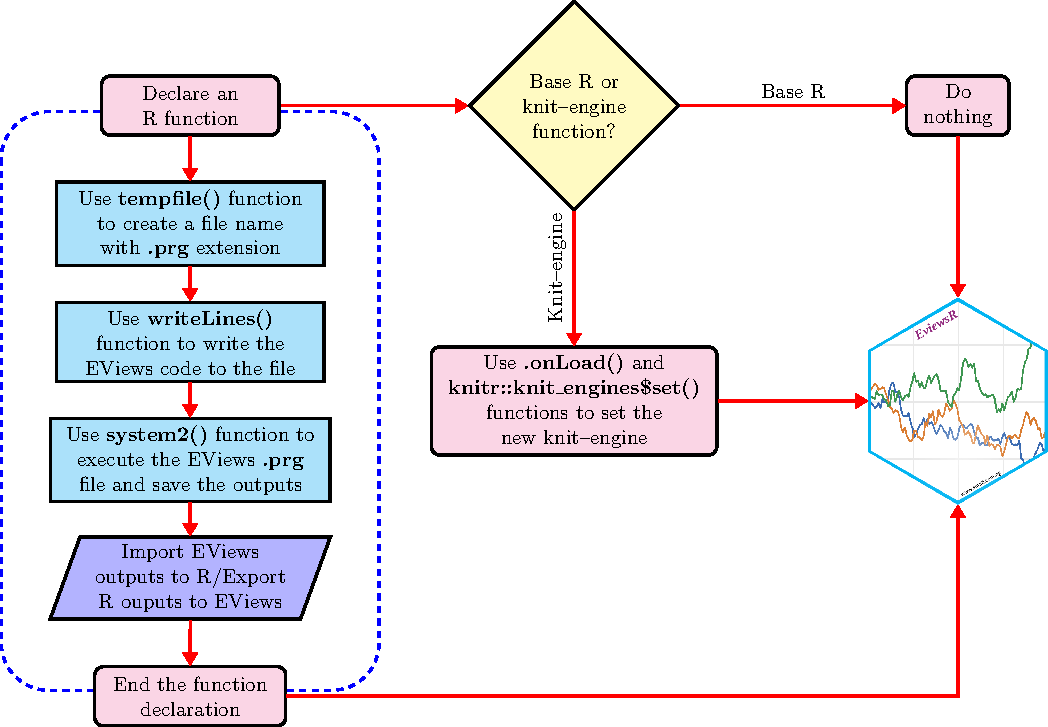
\includegraphics[height=0.35\textheight]{EviewsR_files/figure-latex/EngineSteps-1} 

}

\caption{Architecture of EviewsR}\label{fig:EngineSteps}
\end{figure}

\hypertarget{sec-conclusion}{%
\section{Summary and Conclusion}\label{sec-conclusion}}

We have provided an overview of the \CRANpkg{EviewsR} package, which allows users to run EViews code in R, R Markdown, and Quarto via R functions or knit-engine. The package provides a convenient and efficient way to integrate EViews and R, two of the most popular software packages for econometrics and statistics. The package offers the ability to run EViews code directly from within R, R Markdown, and Quarto, without having to switch between software packages. It also allows users to access and manipulate EViews objects from within R, making it easy to combine EViews analysis with other R-based workflows. In addition, it can be used to generate high-quality reports and presentations using R Markdown and Quarto, with EViews results seamlessly embedded. The package is a valuable tool for economists, statisticians, and other researchers who need to use both software packages.

The \CRANpkg{EviewsR} package is still under development, and there are a number of potential future directions. One possibility is to incorporate graph templates similar to \CRANpkg{ggplot2}'s themes.

We encourage users to provide feedback and suggestions for the \CRANpkg{EviewsR} package, so that it can continue to be improved and meet the needs of the community.

Similar packages include \CRANpkg{URooTab} (\protect\hyperlink{ref-Mati2023a}{Mati 2023}) , \CRANpkg{DynareR} (\protect\hyperlink{ref-Mati2019a}{Mati 2019a}) and \CRANpkg{gretlR} (\protect\hyperlink{ref-Mati2019b}{Mati 2019c}).

\hypertarget{acknowledgements}{%
\section*{Acknowledgements}\label{acknowledgements}}
\addcontentsline{toc}{section}{Acknowledgements}

We are grateful to \href{https://yihui.name/}{Yihui Xie} for creating the \CRANpkg{knitr} package and making his book freely available on-line. We are also grateful to Bob Rudis for explaining how to easily add \texttt{Go} knit-engine to \CRANpkg{knitr}.

\bibliography{EviewsR}

\clearpage

\appendix

\hypertarget{appendix}{%
\section*{APPENDIX}\label{appendix}}
\addcontentsline{toc}{section}{APPENDIX}

\hypertarget{eviews-examples-using-base-r-functions}{%
\section{EViews examples using base R functions}\label{eviews-examples-using-base-r-functions}}

We provide the base R equivalent operations of examples provided by EViews user manual (\url{https://www.eviews.com/help/helpintro.html}).

\hypertarget{eviews-graph-command}{%
\subsection{EViews graph command}\label{eviews-graph-command}}

\url{https://eviews.com/help/helpintro.html\#page/content\%2Fcgraphs-Creating_a_Graph.html}

\hypertarget{example-1}{%
\subsubsection{Example 1}\label{example-1}}

\begin{verbatim}
EViews> line income
\end{verbatim}

\begin{verbatim}
R> eviews_graph(wf = "EviewsR_files/EviewsR", series = "income")
\end{verbatim}

\hypertarget{example-2}{%
\subsubsection{Example 2}\label{example-2}}

\begin{verbatim}
EViews> bar cons
\end{verbatim}

\begin{verbatim}
R> eviews_graph(wf = "EviewsR_files/EviewsR", series = "income",
+     graph_command = "bar")
\end{verbatim}

\hypertarget{example-3}{%
\subsubsection{Example 3}\label{example-3}}

\begin{verbatim}
EViews> scat x y z
\end{verbatim}

\begin{verbatim}
R> eviews_graph(wf = "EviewsR_files/EviewsR", series = "x y z",
+     group = TRUE, graph_command = "scat")
\end{verbatim}

\hypertarget{example-4}{%
\subsubsection{Example 4}\label{example-4}}

\begin{verbatim}
EViews> bar(rotate) cons
\end{verbatim}

\begin{verbatim}
R> eviews_graph(wf = "EviewsR_files/EviewsR", series = "cons", graph_command = "bar",
+     graph_options = "rotate")
\end{verbatim}

Or

\begin{verbatim}
R> eviews_graph(wf = "EviewsR_files/EviewsR", series = "cons", graph_command = "bar(rotate)")
\end{verbatim}

\hypertarget{example-5}{%
\subsubsection{Example 5}\label{example-5}}

\begin{verbatim}
EViews> scat(ab=boxplot) x y z
\end{verbatim}

\begin{verbatim}
R> eviews_graph(wf = "EviewsR_files/EviewsR", series = "x y z",
+     group = TRUE, graph_command = "scat", graph_options = "ab=boxplot")
\end{verbatim}

Or

\begin{verbatim}
R> eviews_graph(wf = "EviewsR_files/EviewsR", series = "x y z",
+     group = TRUE, graph_command = "scat(ab=boxplot)")
\end{verbatim}

\hypertarget{example-6}{%
\subsubsection{Example 6}\label{example-6}}

\begin{verbatim}
EViews> ser2.area(n)
\end{verbatim}

\begin{verbatim}
R> eviews_graph(wf = "EviewsR_files/EviewsR", series = "ser2", graph_command = "area",
+     graph_options = "n")
\end{verbatim}

Or

\begin{verbatim}
R> eviews_graph(wf = "EviewsR_files/EviewsR", series = "ser2", graph_command = "area(n)")
\end{verbatim}

\hypertarget{example-7}{%
\subsubsection{Example 7}\label{example-7}}

\begin{verbatim}
EViews> grp6.xypair
\end{verbatim}

\begin{verbatim}
R> eviews_graph(wf = "EviewsR_files/EviewsR", series = "series1 series2",
+     group = TRUE, graph_command = "xypair")
\end{verbatim}

\hypertarget{example-8}{%
\subsubsection{Example 8}\label{example-8}}

\begin{verbatim}
EViews> group g1 x y z
EViews> g1.scat
\end{verbatim}

\begin{verbatim}
R> eviews_graph(wf = "EviewsR_files/EviewsR", series = "x y z",
+     group = TRUE, graph_command = "scat")
\end{verbatim}

\hypertarget{example-9}{%
\subsubsection{Example 9}\label{example-9}}

Since EViews \texttt{graph} and \texttt{freeze} commands create a graph object on the current EViews workfile, we have use \texttt{exec\_commands()} function instead of \texttt{eviews\_graph()} function. However, if we want to include the graph in an R Markdown or Quarto document, we have to use \texttt{import\_graph()} function.

\begin{verbatim}
EViews> freeze grp6.xypair(m)
\end{verbatim}

\begin{verbatim}
R> exec_commands(commands = "freeze grp6.xypair(m)", wf = "EviewsR_files/EviewsR")
\end{verbatim}

\hypertarget{example-10}{%
\subsubsection{Example 10}\label{example-10}}

\begin{verbatim}
EViews> freeze(graph1) grp6.line
\end{verbatim}

\begin{verbatim}
R> exec_commands(commands = "freeze(graph1) grp6.line", wf = "EviewsR_files/EviewsR")
\end{verbatim}

\hypertarget{example-11}{%
\subsubsection{Example 11}\label{example-11}}

\begin{verbatim}
EViews> graph gr1 ser1 ser2
\end{verbatim}

\begin{verbatim}
R> exec_commands(commands = "graph gr1 ser1 ser2", wf = "EviewsR_files/EviewsR")
\end{verbatim}

\hypertarget{example-12}{%
\subsubsection{Example 12}\label{example-12}}

\begin{verbatim}
EViews> graph gr2.line ser1 ser2
\end{verbatim}

\begin{verbatim}
R> exec_commands(commands = "graph gr2.line ser1 ser2", wf = "EviewsR_files/EviewsR")
\end{verbatim}

\hypertarget{example-13}{%
\subsubsection{Example 13}\label{example-13}}

\begin{verbatim}
EViews> graph gr3.xyline group3
\end{verbatim}

\begin{verbatim}
R> exec_commands(commands = "graph gr3.xyline group3", wf = "EviewsR_files/EviewsR")
\end{verbatim}

\hypertarget{example-14}{%
\subsubsection{Example 14}\label{example-14}}

\begin{verbatim}
EViews> graph g1.xyline(d) unemp gdp inv
\end{verbatim}

\begin{verbatim}
R> exec_commands(commands = "graph g1.xyline(d) unemp gdp inv",
+     wf = "EviewsR_files/EviewsR")
\end{verbatim}

\hypertarget{example-15}{%
\subsubsection{Example 15}\label{example-15}}

\begin{verbatim}
EViews> group grp1 sales1 sales2
EViews> graph grsales.bar(s) grp1
EViews> show grsales
\end{verbatim}

\begin{verbatim}
R> commands = "
+ group grp1 sales1 sales2
+ graph grsales.bar(s) grp1
+ show grsales
+ "
R> 
R> exec_commands(commands = commands, wf = "EviewsR_files/EviewsR")
\end{verbatim}

\hypertarget{example-16}{%
\subsubsection{Example 16}\label{example-16}}

\begin{verbatim}
EViews> graph gr2.merge gr1 grsales
\end{verbatim}

\begin{verbatim}
R> exec_commands(commands = "graph gr2.merge gr1 grsales", wf = "EviewsR_files/EviewsR")
\end{verbatim}

\hypertarget{eviews-import-command}{%
\subsection{EViews import command}\label{eviews-import-command}}

\url{https://www.eviews.com/help/helpintro.html\#page/content\%2Fcommandcmd-import.html}

\hypertarget{example-1-1}{%
\subsubsection{Example 1}\label{example-1-1}}

\begin{verbatim}
EViews> import c:\temp\quarterly.xls @freq q 1990
\end{verbatim}

\begin{verbatim}
R> eviews_import(source_description = "c:\\temp\\quarterly.xls",
+     frequency = "q", start_date = 1990)
\end{verbatim}

\hypertarget{example-2-1}{%
\subsubsection{Example 2}\label{example-2-1}}

\begin{verbatim}
EViews> import(c=s) c:\temp\quarterly.xls range="GDP_SHEET" @freq q 1990 @rename gdp_per_capita gdp
\end{verbatim}

\begin{verbatim}
R> eviews_import(source_description = "c:\\temp\\quarterly.xls range=\"GDP_SHEET\"",
+     options = "c=s", frequency = "q", start_date = 1990, rename_string = "gdp_per_capita gdp")
\end{verbatim}

\hypertarget{example-3-1}{%
\subsubsection{Example 3}\label{example-3-1}}

\begin{verbatim}
EViews> import(mode=p) c:\temp\annual.txt @freq a 1990 @smpl 1994 1996
\end{verbatim}

\begin{verbatim}
R> eviews_import(source_description = "c:\\temp\\annual.txt", options = "mode=p",
+     frequency = "a", start_date = 1990, smpl_string = "1994 1996")
\end{verbatim}

\hypertarget{example-4-1}{%
\subsubsection{Example 4}\label{example-4-1}}

\begin{verbatim}
EViews> import(c=max, type=excel) c:\data\stateunemp.xls @id states @destid states
\end{verbatim}

\begin{verbatim}
R> eviews_import(source_description = "c:\\data\\stateunemp.xls",
+     type = "excel", options = "c=max", id = "states", destid = "states")
\end{verbatim}

\hypertarget{example-5-1}{%
\subsubsection{Example 5}\label{example-5-1}}

\begin{verbatim}
EViews> import c:\data\stategdp.txt colhead=3 delim=comma @id states @date(year) @destid states @date
\end{verbatim}

\begin{verbatim}
R> eviews_import(source_description = "c:\\data\\stategdp.txt colhead=3 delim=comma",
+     id = "states @date(year)", destid = "states @date")
\end{verbatim}

\hypertarget{example-6-1}{%
\subsubsection{Example 6}\label{example-6-1}}

\begin{verbatim}
EViews> import c:\data\cagdp.xls @id states @date(year) @destid states @date @genr states="CA"
\end{verbatim}

\begin{verbatim}
R> eviews_import(source_description = " c:\\data\\cagdp.xls", id = "states @date(year)",
+     destid = "states @date", genr_string = "states=\"CA\"")
\end{verbatim}

\hypertarget{example-7-1}{%
\subsubsection{Example 7}\label{example-7-1}}

\begin{verbatim}
EViews> import(resize) sales.dta @smpl @all
\end{verbatim}

\begin{verbatim}
R> eviews_import(wf = "EviewsR_files/EviewsR", source_description = "sale.dta")
\end{verbatim}

\hypertarget{example-8-1}{%
\subsubsection{Example 8}\label{example-8-1}}

\begin{verbatim}
EViews> import(page=demand) demand.txt @append
\end{verbatim}

\begin{verbatim}
R> eviews_import(wf = "EviewsR_files/EviewsR", source_description = "demand.txt",
+     options = "page=demand", append = TRUE)
\end{verbatim}

\hypertarget{eviews-wfcreate-command}{%
\subsection{EViews wfcreate command}\label{eviews-wfcreate-command}}

\url{https://www.eviews.com/help/helpintro.html\#page/content\%2Fcommandcmd-wfcreate.html}

\hypertarget{example-1-2}{%
\subsubsection{Example 1}\label{example-1-2}}

\begin{verbatim}
EViews> wfcreate(wf=storehours) 30MIN(1-6, 8:00-17:00) 1/3/2000 12/30/2000
\end{verbatim}

\begin{verbatim}
R> eviews_wfcreate(wf = "storehours", frequency = "30MIN", subperiod_opts = "1-6, 8:00-17:00",
+     start_date = "1/3/2000", end_date = "12/30/2000")
\end{verbatim}

Or

\begin{verbatim}
R> eviews_wfcreate(wf = "storehours", frequency = "30MIN(1-6, 8:00-17:00)",
+     start_date = "1/3/2000", end_date = "12/30/2000")
\end{verbatim}

\hypertarget{example-2-2}{%
\subsubsection{Example 2}\label{example-2-2}}

\begin{verbatim}
EViews> wfcreate(wf=storehours) 30MIN(1-6, 8AM-5PM) 1/3/2000 12/30/2000
\end{verbatim}

\begin{verbatim}
R> eviews_wfcreate(wf = "storehours", frequency = "30MIN", subperiod_opts = "1-6, 8AM-5PM",
+     start_date = "1/3/2000", end_date = "12/30/2000")
\end{verbatim}

Or

\begin{verbatim}
R> eviews_wfcreate(wf = "storehours", frequency = "30MIN(1-6, 8AM-5PM)",
+     start_date = "1/3/2000", end_date = "12/30/2000")
\end{verbatim}

\hypertarget{example-3-2}{%
\subsubsection{Example 3}\label{example-3-2}}

\begin{verbatim}
EViews> wfcreate(wf=storehours) 30MIN(1-7, 10AM-3PM) 1/3/2000 12/30/2000
\end{verbatim}

\begin{verbatim}
R> eviews_wfcreate(wf = "storehours", frequency = "30MIN", subperiod_opts = "1-7, 10AM-3PM",
+     start_date = "1/3/2000", end_date = "12/30/2000")
\end{verbatim}

Or

\begin{verbatim}
R> eviews_wfcreate(wf = "storehours", frequency = "30MIN(1-7, 10AM-3PM)",
+     start_date = "1/3/2000", end_date = "12/30/2000")
\end{verbatim}

\hypertarget{example-4-2}{%
\subsubsection{Example 4}\label{example-4-2}}

\begin{verbatim}
EViews> wfcreate(wf=storehours) 30MIN(1-6, 8AM-5PM) 1/3/2000 10AM 12/30/2000 2PM
\end{verbatim}

\begin{verbatim}
R> eviews_wfcreate(wf = "storehours", frequency = "30MIN", subperiod_opts = "1-6, 8AM-5PM",
+     start_date = "1/3/2000 10AM", end_date = "12/30/2000 2PM")
\end{verbatim}

Or

\begin{verbatim}
R> eviews_wfcreate(wf = "storehours", frequency = "30MIN(1-6, 8AM-5PM)",
+     start_date = "1/3/2000 10AM", end_date = "12/30/2000 2PM")
\end{verbatim}

\hypertarget{example-5-2}{%
\subsubsection{Example 5}\label{example-5-2}}

\begin{verbatim}
EViews> wfcreate w(monday) 2000 2010
\end{verbatim}

\begin{verbatim}
R> eviews_wfcreate(frequency = "W", subperiod_opts = "monday", start_date = "2000",
+     end_date = "2010")
\end{verbatim}

Or

\begin{verbatim}
R> eviews_wfcreate(frequency = "W(monday)", start_date = "2000",
+     end_date = "2010")
\end{verbatim}

\hypertarget{example-6-2}{%
\subsubsection{Example 6}\label{example-6-2}}

\begin{verbatim}
EViews> wfcreate a(july) 2001 2007
\end{verbatim}

\begin{verbatim}
R> eviews_wfcreate(frequency = "a", subperiod_opts = "july", start_date = "2001",
+     end_date = "2007")
\end{verbatim}

Or

\begin{verbatim}
R> eviews_wfcreate(frequency = "a(july)", start_date = "2001", end_date = "2007")
\end{verbatim}

\hypertarget{example-7-2}{%
\subsubsection{Example 7}\label{example-7-2}}

\begin{verbatim}
EViews> wfcreate w 2000 2010
\end{verbatim}

\begin{verbatim}
R> eviews_wfcreate(frequency = "W", start_date = "2000", end_date = "2010")
\end{verbatim}

\hypertarget{example-8-2}{%
\subsubsection{Example 8}\label{example-8-2}}

\begin{verbatim}
EViews> wfcreate(wf=annual, page=myproject) a 1950 2005
\end{verbatim}

\begin{verbatim}
R> eviews_wfcreate(wf = "annual", page = "myproject", frequency = "a",
+     start_date = "1950", end_date = "2005")
\end{verbatim}

\hypertarget{example-9-1}{%
\subsubsection{Example 9}\label{example-9-1}}

\begin{verbatim}
EViews> wfcreate(wf=unstruct, page=undated) u 1000
\end{verbatim}

\begin{verbatim}
R> eviews_wfcreate(wf = "unstruct", page = "undated", frequency = "u",
+     num_observations = 1000)
\end{verbatim}

\hypertarget{example-10-1}{%
\subsubsection{Example 10}\label{example-10-1}}

\begin{verbatim}
EViews> wfcreate(wf=griliches_grunfeld, page=annual) a 1935 1954 10
\end{verbatim}

\begin{verbatim}
R> eviews_wfcreate(wf = "griliches_grunfeld", page = "annual", frequency = "a",
+     start_date = 1935, end_date = 1954, num_cross_sections = 10)
\end{verbatim}

\hypertarget{example-11-1}{%
\subsubsection{Example 11}\label{example-11-1}}

\begin{verbatim}
EViews> wfcreate(wf=fourday) D(1,4) 1/3/2000 12/31/2000
\end{verbatim}

\begin{verbatim}
R> eviews_wfcreate(wf = "fourday", frequency = "D", subperiod_opts = "1,4",
+     start_date = "1/3/2000", end_date = "12/31/2000")
\end{verbatim}

Or

\begin{verbatim}
R> eviews_wfcreate(wf = "fourday", frequency = "D(1,4)", start_date = "1/3/2000",
+     end_date = "12/31/2000")
\end{verbatim}

\hypertarget{example-12-1}{%
\subsubsection{Example 12}\label{example-12-1}}

\begin{verbatim}
EViews> wfcreate(wf=fourday) D(1-4) 1/3/2000 12/31/2000
\end{verbatim}

\begin{verbatim}
R> eviews_wfcreate(wf = "fourday", frequency = "D", subperiod_opts = "1-4",
+     start_date = "1/3/2000", end_date = "12/31/2000")
\end{verbatim}

Or

\begin{verbatim}
R> eviews_wfcreate(wf = "fourday", frequency = "D(1-4)", start_date = "1/3/2000",
+     end_date = "12/31/2000")
\end{verbatim}

\hypertarget{example-13-1}{%
\subsubsection{Example 13}\label{example-13-1}}

\begin{verbatim}
EViews> wfcreate(wf=captimes) 15SEC(2-4) 1/3/2000 12/30/2000
\end{verbatim}

\begin{verbatim}
R> eviews_wfcreate(wf = "captimes", frequency = "15SEC", subperiod_opts = "2-4",
+     start_date = "1/3/2000", end_date = "12/31/2000")
\end{verbatim}

Or

\begin{verbatim}
R> eviews_wfcreate(wf = "captimes", frequency = "15SEC(2-4)", start_date = "1/3/2000",
+     end_date = "12/31/2000")
\end{verbatim}

\hypertarget{example-14-1}{%
\subsubsection{Example 14}\label{example-14-1}}

\begin{verbatim}
EViews> wfcreate m 1995 +30
\end{verbatim}

\begin{verbatim}
R> eviews_wfcreate(frequency = "m", start_date = "1995", end_date = "+30")
\end{verbatim}

\hypertarget{eviews-pagesave-command}{%
\subsection{EViews pagesave command}\label{eviews-pagesave-command}}

\url{https://eviews.com/help/helpintro.html\#page/content\%2Fcommandcmd-pagesave.html}

\hypertarget{example-1-3}{%
\subsubsection{Example 1}\label{example-1-3}}

\begin{verbatim}
EViews> pagesave new_wf
\end{verbatim}

\begin{verbatim}
R> eviews_pagesave(wf = "EviewsR_files/EviewsR", source_description = "new_wf")
\end{verbatim}

\hypertarget{example-2-3}{%
\subsubsection{Example 2}\label{example-2-3}}

\begin{verbatim}
EViews> pagesave "c:\documents and settings\my data\consump"
\end{verbatim}

\begin{verbatim}
R> eviews_pagesave(wf="EviewsR_files/EviewsR",
+                 source_description = "c:\\documents and settings\\my data\\consump")
\end{verbatim}

\hypertarget{example-3-3}{%
\subsubsection{Example 3}\label{example-3-3}}

\begin{verbatim}
EViews> pagesave macro @keep gdp unemp
\end{verbatim}

\begin{verbatim}
R> eviews_pagesave(wf = "EviewsR_files/EviewsR", source_description = "macro",
+     keep_list = "gdp unemp")
\end{verbatim}

\hypertarget{example-4-3}{%
\subsubsection{Example 4}\label{example-4-3}}

\begin{verbatim}
EViews> pagesave macro @dropmap gdp*
\end{verbatim}

\begin{verbatim}
R> eviews_pagesave(wf = "EviewsR_files/EviewsR", source_description = "macro",
+     dropmap_list = "gdp*")
\end{verbatim}

\hypertarget{example-5-3}{%
\subsubsection{Example 5}\label{example-5-3}}

\begin{verbatim}
EViews> pagesave(type=excelxml, mode=update) macro.xlsx
\end{verbatim}

\begin{verbatim}
R> eviews_pagesave(wf = "EviewsR_files/EviewsR", options = "type=excelxml,mode=update",
+     source_description = "macro.xlsx")
\end{verbatim}

\hypertarget{example-6-3}{%
\subsubsection{Example 6}\label{example-6-3}}

\begin{verbatim}
EViews> pagesave(type=excelxml, mode=update) macro.xlsx range="Sheet2!a1" byrow @keep gdp unemp
\end{verbatim}

\begin{verbatim}
R> eviews_pagesave(wf = "EviewsR_files/EviewsR", options = "type=excelxml,mode=update",
+     source_description = "macro.xlsx", table_description = "range=\"sheet2!a1\" byrow",
+     keep_list = "gdp unemp")
\end{verbatim}

\hypertarget{example-7-3}{%
\subsubsection{Example 7}\label{example-7-3}}

\begin{verbatim}
EViews> pagesave(type=excelxml, mode=update) macro.xlsm range="Sheet2!a1" byrow @keep gdp unemp
\end{verbatim}

\begin{verbatim}
R> eviews_pagesave(wf = "EviewsR_files/EviewsR", options = "type=excelxml,mode=update",
+     source_description = "macro.xlsm", table_description = "range=\"sheet2!a1\"",
+     keep_list = "gdp unemp")
\end{verbatim}

\hypertarget{example-8-3}{%
\subsubsection{Example 8}\label{example-8-3}}

\begin{verbatim}
EViews> pagesave(type=excelxml, noid) macro.xlsx range="Sheet2!a1"
\end{verbatim}

\begin{verbatim}
R> eviews_pagesave(wf = "EviewsR_files/EviewsR", options = "type=excelxml,noid",
+     source_description = "macro.xlsx", table_description = "range=\"sheet2!a1\"")
\end{verbatim}

\hypertarget{eviews-wfsave-command}{%
\subsection{EViews wfsave command}\label{eviews-wfsave-command}}

\url{https://eviews.com/help/helpintro.html\#page/content\%2Fcommandcmd-wfsave.html}

The EViews commands \texttt{pagesave} and \texttt{wfsave} are similar. Therefore, the above examples about \texttt{pagesave} can be adopted by replacing \texttt{pagesave} with \texttt{wfsave}.

\hypertarget{notes-for-eviews-users}{%
\section{Notes for EViews users}\label{notes-for-eviews-users}}

This section explains some peculiarities of R's syntax. It is important for working with \CRANpkg{EviewsR}'s functions.

Each of the following is valid way to write a character string containing double quote (\texttt{"}). All of them assign the same string (\texttt{range="sheet2!a1"\ byrow}) to \texttt{table\_description}.

\begin{verbatim}
R> table_description='range="sheet2!a1" byrow'
R> table_descriptione="range=\"sheet2!a1\" byrow"
R> table_description=r'(range="sheet2!a1" byrow)'
R> table_description=r"(range="sheet2!a1" byrow)"
\end{verbatim}

Similarly, we can write string with single quote (\texttt{\textquotesingle{}}) as follows:

\begin{verbatim}
R> table_description='range=\'sheet2!a1\' byrow'
R> table_descriptione="range='sheet2!a1' byrow"
R> table_description=r'(range='sheet2!a1' byrow)'
R> table_description=r"(range='sheet2!a1' byrow)"
\end{verbatim}

\begin{verbatim}
R> set_eviews_path("C:/Program Files (x86)/EViews 10/EViews10.exe")
R> set_eviews_path("C:\\Program Files (x86)\\EViews 10\\EViews10.exe")
R> set_eviews_path(r'(C:\Program Files (x86)\EViews 10\EViews10.exe)')
R> set_eviews_path(r"(C:\Program Files (x86)\EViews 10\EViews10.exe)")
\end{verbatim}

Therefore, we recommend using \texttt{r\textquotesingle{}()\textquotesingle{}} or \texttt{r"()"} to write complex strings, as both return the strings written between the braces exactly as they are.

\hypertarget{current-knitr-knit-engines}{%
\section{Current knitr knit-engines}\label{current-knitr-knit-engines}}

This section provides the list of knit-engines that are currently available as of November 01, 2023. Please note that \texttt{eviews} is included among the list because \CRANpkg{EviewsR} has added it as a knit-engine.

\begin{verbatim}
#>  [1] "awk"         "bash"        "coffee"      "gawk"        "groovy"     
#>  [6] "haskell"     "lein"        "mysql"       "node"        "octave"     
#> [11] "perl"        "php"         "psql"        "Rscript"     "ruby"       
#> [16] "sas"         "scala"       "sed"         "sh"          "stata"      
#> [21] "zsh"         "asis"        "asy"         "block"       "block2"     
#> [26] "bslib"       "c"           "cat"         "cc"          "comment"    
#> [31] "css"         "ditaa"       "dot"         "embed"       "eviews"     
#> [36] "exec"        "fortran"     "fortran95"   "go"          "highlight"  
#> [41] "js"          "julia"       "python"      "R"           "Rcpp"       
#> [46] "sass"        "scss"        "sql"         "stan"        "targets"    
#> [51] "tikz"        "verbatim"    "glue"        "glue_sql"    "gluesql"    
#> [56] "theorem"     "lemma"       "corollary"   "proposition" "conjecture" 
#> [61] "definition"  "example"     "exercise"    "hypothesis"  "proof"      
#> [66] "remark"      "solution"
\end{verbatim}

\hypertarget{session-information}{%
\section{Session information}\label{session-information}}

This section provides detailed information on the Operating System, R packages and their versions used in this document.

\begin{verbatim}
#> R version 4.2.2 (2022-10-31)
#> Platform: aarch64-apple-darwin20 (64-bit)
#> Running under: macOS 14.0
#> 
#> Matrix products: default
#> BLAS:   /Library/Frameworks/R.framework/Versions/4.2-arm64/Resources/lib/libRblas.0.dylib
#> LAPACK: /Library/Frameworks/R.framework/Versions/4.2-arm64/Resources/lib/libRlapack.dylib
#> 
#> locale:
#> [1] en_US.UTF-8/en_US.UTF-8/en_US.UTF-8/C/en_US.UTF-8/en_US.UTF-8
#> 
#> attached base packages:
#> [1] grid      stats     graphics  grDevices utils     datasets  methods  
#> [8] base     
#> 
#> other attached packages:
#> [1] magrittr_2.0.3   ggplot2_3.4.3    Gmisc_3.0.3      htmlTable_2.4.1 
#> [5] Rcpp_1.0.11      kableExtra_1.3.4 knitr_1.45       EviewsR_0.1.5   
#> 
#> loaded via a namespace (and not attached):
#>  [1] lubridate_1.9.3     svglite_2.1.1       lattice_0.21-9     
#>  [4] zoo_1.8-12          digest_0.6.33       utf8_1.2.3         
#>  [7] R6_2.5.1            backports_1.4.1     evaluate_0.22      
#> [10] httr_1.4.7          pillar_1.9.0        rlang_1.1.1        
#> [13] data.table_1.14.8   rstudioapi_0.15.0   rpart_4.1.19       
#> [16] checkmate_2.2.0     rmarkdown_2.25      webshot_0.5.5      
#> [19] stringr_1.5.0       foreign_0.8-85      htmlwidgets_1.6.2  
#> [22] tinytex_0.47        munsell_0.5.0       hunspell_3.0.3     
#> [25] compiler_4.2.2      xfun_0.40           pkgconfig_2.0.3    
#> [28] systemfonts_1.0.4   base64enc_0.1-3     htmltools_0.5.6.1  
#> [31] nnet_7.3-19         forestplot_3.1.3    tidyselect_1.2.0   
#> [34] gridExtra_2.3       tibble_3.2.1        bookdown_0.35      
#> [37] rjtools_1.0.12      Hmisc_5.1-1         XML_3.99-0.14      
#> [40] fansi_1.0.5         viridisLite_0.4.2   withr_2.5.1        
#> [43] dplyr_1.1.3         gtable_0.3.4        lifecycle_1.0.3    
#> [46] formatR_1.14        scales_1.2.1        cli_3.6.1          
#> [49] stringi_1.7.12      fs_1.6.3            xml2_1.3.5         
#> [52] xts_0.13.1          yesno_0.1.2         vctrs_0.6.3        
#> [55] generics_0.1.3      Formula_1.2-5       tools_4.2.2        
#> [58] glue_1.6.2          purrr_1.0.2         abind_1.4-5        
#> [61] fastmap_1.1.1       yaml_2.3.7          timechange_0.2.0   
#> [64] colorspace_2.1-0    cluster_2.1.4       BiocManager_1.30.22
#> [67] rvest_1.0.3
\end{verbatim}

\clearpage

\hypertarget{references}{%
\section*{References}\label{references}}
\addcontentsline{toc}{section}{References}

\hypertarget{refs}{}
\begin{CSLReferences}{1}{0}
\leavevmode\vadjust pre{\hypertarget{ref-rmarkdown}{}}%
Allaire, JJ, Yihui Xie, Jonathan McPherson, Javier Luraschi, Kevin Ushey, Aron Atkins, Hadley Wickham, Joe Cheng, Winston Chang, and Richard Iannone. 2020. \emph{Rmarkdown: Dynamic Documents for r}. \url{https://github.com/rstudio/rmarkdown}.

\leavevmode\vadjust pre{\hypertarget{ref-christensen2018}{}}%
Christensen, Garret, and Edward Miguel. 2018. {``Transparency, Reproducibility, and the Credibility of Economics Research.''} \emph{Journal of Economic Literature} 56 (3): 920--80. \url{https://doi.org/10.1257/jel.20171350}.

\leavevmode\vadjust pre{\hypertarget{ref-franco2014}{}}%
Franco, Annie, Neil Malhotra, and Gabor Simonovits. 2014. {``Publication Bias in the Social Sciences: Unlocking the File Drawer.''} \emph{Science} 345 (6203): 1502--5. \url{https://doi.org/10.1126/science.1255484}.

\leavevmode\vadjust pre{\hypertarget{ref-gerber2014}{}}%
Gerber, Alan, Kevin Arceneaux, Cheryl Boudreau, Conor Dowling, Sunshine Hillygus, Thomas Palfrey, Daniel R. Biggers, and David J. Hendry. 2014. {``Reporting Guidelines for Experimental Research: A Report from the Experimental Research Section Standards Committee.''} \emph{Journal of Experimental Political Science} 1 (1): 81--98. \url{https://doi.org/10.1017/xps.2014.11}.

\leavevmode\vadjust pre{\hypertarget{ref-harvey2015}{}}%
Harvey, Campbell R., Yan Liu, and Heqing Zhu. 2015. {``{\ldots{} and the Cross-Section of Expected Returns}.''} \emph{The Review of Financial Studies} 29 (1): 5--68. \url{https://doi.org/10.1093/rfs/hhv059}.

\leavevmode\vadjust pre{\hypertarget{ref-ioannidis2005}{}}%
Ioannidis, John P. A. 2005. {``Why Most Published Research Findings Are False.''} \emph{PLOS Medicine} 2 (8). \url{https://doi.org/10.1371/journal.pmed.0020124}.

\leavevmode\vadjust pre{\hypertarget{ref-Mati2019a}{}}%
Mati, Sagiru. 2019a. \emph{DynareR: Bringing the Power of {Dynare to R, R Markdown, and Quarto}}. \url{https://CRAN.R-project.org/package=DynareR}.

\leavevmode\vadjust pre{\hypertarget{ref-Mati2019}{}}%
---------. 2019b. \emph{EviewsR: A Seamless Integration of {EViews} and {R}}. \url{https://CRAN.R-project.org/package=EviewsR}.

\leavevmode\vadjust pre{\hypertarget{ref-Mati2019b}{}}%
---------. 2019c. \emph{gretlR: A Seamless Integration of {Gretl} and {R}}. \url{https://CRAN.R-project.org/package=gretlR}.

\leavevmode\vadjust pre{\hypertarget{ref-Mati2023a}{}}%
---------. 2023. \emph{{URooTab}: Tabular Reporting of {EViews} Unit Root Tests}. CRAN. \url{https://CRAN.R-project.org/package=EviewsR}.

\leavevmode\vadjust pre{\hypertarget{ref-Mati2023}{}}%
Mati, Sagiru, Irfan Civcir, and Huseyin Ozdeser. 2023. {``{ECOWAS} Common Currency, a Mirage or Possibility?''} \emph{Panoeconomicus}, 1--25. \url{https://doi.org/10.2298/PAN191119015M}.

\leavevmode\vadjust pre{\hypertarget{ref-Mati2019c}{}}%
Mati, Sagiru, Irfan Civcir, and Hüseyin Ozdeser. 2019. {``{ECOWAS} Common Currency: How Prepared Are Its Members?''} \emph{Investigación Económica} 78 (May): 89. \url{https://doi.org/10.22201/fe.01851667p.2019.308.69625}.

\leavevmode\vadjust pre{\hypertarget{ref-paul2019}{}}%
Murrell, Paul. 2019. \emph{\pkg{hexView}: Viewing Binary Files}. \url{https://CRAN.R-project.org/package=hexView}.

\leavevmode\vadjust pre{\hypertarget{ref-felix2018}{}}%
Pretis, Felix, J. James Reade, and Genaro Sucarrat. 2018. {``Automated General-to-Specific (\pkg{GETS}) Regression Modeling and Indicator Saturation for Outliers and Structural Breaks.''} \emph{Journal of Statistical Software} 86 (3): 1--44. \url{https://doi.org/10.18637/jss.v086.i03}.

\leavevmode\vadjust pre{\hypertarget{ref-R}{}}%
R Core Team. 2019. \emph{R: A Language and Environment for Statistical Computing}. Vienna, Austria: R Foundation for Statistical Computing. \url{https://www.R-project.org/}.

\leavevmode\vadjust pre{\hypertarget{ref-sandve2013}{}}%
Sandve, Anton AND Taylor, Geir Kjetil AND Nekrutenko. 2013. {``Ten Simple Rules for Reproducible Computational Research.''} \emph{PLOS Computational Biology} 9 (10): 1--4. \url{https://doi.org/10.1371/journal.pcbi.1003285}.

\leavevmode\vadjust pre{\hypertarget{ref-joseph2011}{}}%
Simmons, Joseph P., Leif D. Nelson, and Uri Simonsohn. 2011. {``False-Positive Psychology: Undisclosed Flexibility in Data Collection and Analysis Allows Presenting Anything as Significant.''} \emph{Psychological Science} 22 (11): 1359--66. \url{https://doi.org/10.1177/0956797611417632}.

\leavevmode\vadjust pre{\hypertarget{ref-Eviews2019}{}}%
Startz, Richard. 2019. {``EViews Illustrated.''} \emph{University of California: Santa Barbara, CA, USA}.

\leavevmode\vadjust pre{\hypertarget{ref-stodden2014}{}}%
Stodden, Victoria, Friedrich Leisch, and Roger D Peng. 2014. \emph{Implementing Reproducible Research}. Crc Press.

\leavevmode\vadjust pre{\hypertarget{ref-Wickham2016}{}}%
Wickham, Hadley. 2016. \emph{Ggplot2: Elegant Graphics for Data Analysis}. Springer-Verlag New York. \url{https://ggplot2.tidyverse.org}.

\leavevmode\vadjust pre{\hypertarget{ref-xie2014}{}}%
Xie, Yihui. 2014. {``\pkg{knitr}: A Comprehensive Tool for Reproducible Research in r.''} In \emph{Implementing Reproducible Computational Research}, edited by Victoria Stodden, Friedrich Leisch, and Roger D. Peng. Chapman; Hall/CRC. \url{http://www.crcpress.com/product/isbn/9781466561595}.

\leavevmode\vadjust pre{\hypertarget{ref-xie2015}{}}%
---------. 2015. \emph{Dynamic Documents with r and \pkg{knitr}}. 2nd ed. Boca Raton, Florida: Chapman; Hall/CRC. \url{https://yihui.name/knitr/}.

\leavevmode\vadjust pre{\hypertarget{ref-xie2019}{}}%
---------. 2019. \emph{\pkg{knitr}: A General-Purpose Package for Dynamic Report Generation in r}. \url{https://yihui.name/knitr/}.

\end{CSLReferences}

\bibliography{RJreferences.bib}

\address{%
Sagiru Mati\\
Near East University\\%
\textsuperscript{1}Operational Research Center in Healthcare\\ Near East University, Nicosia, North Cyprus\\ \textsuperscript{2}Department of Economics\\ Yusuf Maitama Sule University, Nigeria\\
%
\url{https://www.smati.com.ng}\\%
\textit{ORCiD: \href{https://orcid.org/0000-0003-1413-3974}{0000-0003-1413-3974}}\\%
\href{mailto:sagirumati@gmail.com}{\nolinkurl{sagirumati@gmail.com}}%
}

\address{%
Irfan Civcir\\
Ankara University\\%
Department of Economics\\ Ankara, Turkey\\
%
\url{http://cv.ankara.edu.tr/kisi.php?id=civcir@politics.ankara.edu.tr&deger=2}\\%
\textit{ORCiD: \href{https://orcid.org/0000-0002-2557-2625}{0000-0002-2557-2625}}\\%
\href{mailto:civcir@politics.ankara.edu.tr}{\nolinkurl{civcir@politics.ankara.edu.tr}}%
}

\address{%
S. I. Abba\\
King Fahd University of Petroleum and Minerals\\%
Interdisciplinary Research Center for Membranes and Water Security\\ Dhahran 31261, Saudi Arabia\\
%
\url{https://scholar.google.com/citations?user=4h2JX7YAAAAJ&hl=en}\\%
\textit{ORCiD: \href{https://orcid.org/0000-0001-9356-2798}{0000-0001-9356-2798}}\\%
\href{mailto:sani.abba@kfupm.edu.sa}{\nolinkurl{sani.abba@kfupm.edu.sa}}%
}
